%% RiSE Latex Template - version 0.5
%%
%% RiSE's latex template for thesis and dissertations
%% http://risetemplate.sourceforge.net
%%
%% (c) 2012 Yguaratã Cerqueira Cavalcanti (yguarata@gmail.com)
%%          Vinicius Cardoso Garcia (vcg@cin.ufpe.br)
%%
%% This document was initially based on UFPEThesis template, from Paulo Gustavo
%% S. Fonseca.
%%
%% ACKNOWLEDGEMENTS
%%
%% We would like to thanks the RiSE's researchers community, the 
%% students from Federal University of Pernambuco, and other users that have
%% been contributing to this projects with comments and patches.
%%
%% GENERAL INSTRUCTIONS
%%
%% We strongly recommend you to compile your documents using pdflatex command.
%% It is also recommend use the texlipse plugin for Eclipse to edit your documents.
%%
%% Options for \documentclass command:
%%         * Idiom
%%           pt   - Portguese (default)
%%           en   - English
%%
%%         * Text type
%%           bsc  - B.Sc. Thesis
%%           msc  - M.Sc. Thesis (default)
%%           qual - PHD qualification (not tested yet)
%%           prop - PHD proposal (not tested yet)
%%           phd  - PHD thesis
%%
%%         * Media
%%           scr  - to eletronic version (PDF) / see the users guide
%%
%%         * Pagination
%%           oneside - unique face press
%%           twoside - two faces press
%%
%%		   * Line spacing
%%           singlespacing  - the same as using \linespread{1}
%%           onehalfspacing - the same as using \linespread{1.3}
%%           doublespacing  - the same as using \linespread{1.6}
%%
%% Reference commands. Use the following commands to make references in your
%% text:
%%          \figref  -- for Figure reference
%%          \tabref  -- for Table reference
%%          \eqnref  -- for equation reference
%%          \chapref -- for chapter reference
%%          \secref  -- for section reference
%%          \appref  -- for appendix reference
%%          \axiref  -- for axiom reference
%%          \conjref -- for conjecture reference
%%          \defref  -- for definition reference
%%          \lemref  -- for lemma reference
%%          \theoref -- for theorem reference
%%          \corref  -- for corollary reference
%%          \propref -- for proprosition reference
%%          \pgref   -- for page reference
%%
%%          Example: See \chapref{chap:introduction}. It will produce 
%%                   'See Chapter 1', in case of English language.
%%
%% Citation commands:
%%          \citet (from natbib) -- To cite a reference as part of the narrative
%%          \citep (from natbib) -- To cite a reference between parenthesis
%%          citationblock environment -- To produce direct citation blocks according to the ABNT

\documentclass[en,twoside,onehalfspacing,msc]{risethesis}

\usepackage{colortbl}
\usepackage{color}
\usepackage[table]{xcolor}
\usepackage{microtype}
\usepackage{bibentry}
\usepackage{subfigure}
\usepackage{multirow}
\usepackage{rotating}
\usepackage{booktabs}
\usepackage{pdfpages}
\usepackage{caption}
\usepackage{lipsum}
\usepackage{sectsty}
\usepackage{listings}
\usepackage{mdframed}

\captionsetup[table]{position=top,justification=centering,width=.85\textwidth,labelfont=bf,font=footnotesize}
\captionsetup[lstlisting]{position=top,justification=centering,width=.85\textwidth,labelfont=bf,font=footnotesize}
\captionsetup[figure]{position=bottom,justification=centering,width=.85\textwidth,labelfont=bf,font=footnotesize}

%% Chapter and (Sub)Section fonts must be same size as text (12)
\sectionfont{\fontsize{12}{15}\selectfont}
\subsectionfont{\fontsize{12}{15}\selectfont}
\subsubsectionfont{\fontsize{12}{15}\selectfont}

%% Change the following pdf author attribute name to your name.
\usepackage[linkcolor=black,
            citecolor=black,
            urlcolor=black,
            colorlinks,
            pdfpagelabels,
            pdftitle={Rise Thesis Template (ABNT)},
            pdfauthor={Rise Thesis Template (ABNT)},
            breaklinks=true]{hyperref}

\address{RECIFE}

\universitypt{Universidade Federal de Pernambuco}
\universityen{Federal University of Pernambuco}

\departmentpt{Centro de Informática}
\departmenten{Center for Informatics}

\programpt{Pós-graduação em Ciência da Computação}
\programen{Graduate in Computer Science}

\majorfieldpt{Ciência da Computação}
\majorfielden{Computer Science}

\title{Test Suite Parallelization in Open Source Projects: A Study on Its Usage and Impact}

\date{2018}

\author{Jeanderson Barros C{â}ndido}
\adviser{Marcelo Bezerra d'Amorim}

% Macros (defines your own macros here, if needed)
\def\x{\checkmark}
% \newcommand{\finalVersion} % Uncomment this line to generate a
% production ready pdf

\ifdefined\finalVersion
    \newcommand{\LineComment}[3]{}
\else
    \newcommand{\LineComment}[3]{\textbf{[[#1}{\color{#2} #3}\textbf{]]}}
\fi

\newcommand{\pef}{PEF}
%% please, do not italicize ``i.e.'' and ``e.g.'' - Marcelo
\newcommand{\ie}{i.e.}
\newcommand{\eg}{e.g.}
\newcommand{\etal}{et al.}
\newcommand{\Comment}[1]{}
\newcommand{\CodeIn}[1]{{\small\texttt{#1}}}

\newcommand{\Fix}[1]{\LineComment{}{red}{#1}}
\newcommand{\Jbc}[1]{\LineComment{Jean: }{orange}{#1}}
\newcommand{\Luis}[1]{\LineComment{Luis: }{darkblue}{#1}}
\newcommand{\Mar}[1]{\LineComment{Marcelo: }{darkgreen}{#1}}

%% use this macros
\newcommand{\github}{Github} %% change consistently
\newcommand{\pomf}{\emph{pom.xml}} %% change consistently

%% Evaluation macros

%% SUBJECTS
\newcommand{\SubjectsGithub}{813}
\newcommand{\SubjectsGithubNotMaven}{\Fix{48}}
\newcommand{\SubjectsGithubNotTestable}{\Fix{132}}
\newcommand{\SubjectsGithubFlaky}{\Fix{16}}
\newcommand{\numSubjs}{390}
\newcommand{\numSubjsShort}{307}
\newcommand{\numSubjsMed}{49}
\newcommand{\numSubjsLong}{34}

%% CONFIGURATION MODES
\newcommand{\Seq}{C0}
\newcommand{\SeqClassParMeth}{C1}
\newcommand{\ParClassSeqMeth}{C2}
\newcommand{\ParClassParMeth}{C3}
\newcommand{\Fork}{F}
\newcommand{\ForkSeq}{\Fork{}\Seq{}}
\newcommand{\ForkParMeth}{\Fork{}\SeqClassParMeth{}}

%% RQ1
\newcommand{\medg}{medium}
\newcommand{\longg}{long}
\newcommand{\shortg}{short}

\newcommand{\numSubjsPass}{250}
\newcommand{\numSubjsFail}{140}

\newcommand{\numMed}{\Fix{49}}
\newcommand{\numLong}{\Fix{34}}
\newcommand{\numMedLong}{83}
\newcommand{\percentMedLongRunning}{21\%}
\newcommand{\percentLongRunning}{8.7\%}

%% RQ3&RQ4
\newcommand{\avgSpeedup}{4.4}
\newcommand{\pomMedLong}{67}
\newcommand{\numPomMed}{38}
\newcommand{\numPomLong}{29}
\newcommand{\numPomMatched}{\pomMedLong{}}
\newcommand{\percentParallel}{13.3\%}
\newcommand{\percentParallelUpdated}{18.1\%}
\newcommand{\numNonParallel}{74}
%% \newcommand{\numPomMatchedValid}{\Fix{103}}
\newcommand{\numProjectsPar}{nine}
\newcommand{\percentShortSequential}{\Fix{96.7\%}}

\newcommand{\averageMedLongRunning}{8m36s}
\newcommand{\percentParallelForLongRunning}{\Fix{80\%}}

%% RQ5
\newcommand{\emailsSent}{297}
\newcommand{\emailsFalseAnswers}{three}
\newcommand{\emailsTrueAnswers}{32}
\newcommand{\emailsProjectsAnswered}{36}
\newcommand{\percEmailsProjectsAnswered}{61.29\%}
\newcommand{\emailsAnswered}{38}
\newcommand{\percEmailsAnswered}{12.8\%}
\newcommand{\discartedProjects}{10}
\newcommand{\emailsProjects}{62}

%% RQ5 Survey answers
\newcommand{\emailsCI}{12} % 8 + distributed
\newcommand{\emailsLocal}{6}
\newcommand{\emailsDistributed}{4}
\newcommand{\emailsNotDescribed}{14}

\newcommand{\emailsSequential}{30}
\newcommand{\emailsParallel}{6}

\newcommand{\emailsA}{8.33\%} %3
\newcommand{\emailsB}{33.33\%} %12
\newcommand{\emailsC}{22.22\%} %8
\newcommand{\emailsD}{16.67\%} %6
\newcommand{\emailsNA}{19.45\%} %7

\newcommand{\webpage}{\url{https://doubleblind.000webhostapp.com/}}


\begin{document}

\frontmatter

\frontpage

\presentationpage

\begin{fichacatalografica}
	\FakeFichaCatalografica % Comment this line when you have the correct file
%     \includepdf{fig_ficha_catalografica.pdf} % Uncomment this
\end{fichacatalografica}

\banca

\begin{dedicatory}
I dedicate this thesis to all my family, friends and professors who gave me the
necessary support to get here.
\end{dedicatory}

\acknowledgements
\lipsum[1-4]

\begin{epigraph}[]{Poul Anderson}
I have yet to see any problem, however complicated, which, when looked at in the
right way, did not become still more complicated.
\end{epigraph}

\resumo
% Escreva seu resumo no arquivo resumo.tex
{\parindent0pt
	O gerenciamento eficiente de solicitações de mudança (SM) é fundamental para o
sucesso das atividades de manutenção e evolução de software. Entretanto, a
atribuição de SMs a desenvolvedores de software é um aspecto custoso desse
gerenciamento, pois demanda tempo e requer conhecimento apropriado do projeto de
software. Com o propósito de diminuir esse custo, várias pesquisas já propuseram
métodos de atribuição automática de SMs. Embora representem avanços na área,
existem vários fatores inerentes a atribuição de SMs que não são considerados
nessas pesquisas e são essenciais para a automação.

Como demonstrado nesse trabalho, a atribuição automática deve, por exemplo,
considerar a carga de trabalho, a experiência e o conhecimento dos
desenvolvedores, a prioridade e a severidade das SMs, a afinidade dos
desenvolvedores com os problemas descritos nas SMs, e até mesmo os
relacionamentos interpessoais. Para tornar esse cenário ainda mais complexo,
esses fatos podem variar de acordo com o projeto de software que está sendo
desenvolvido. Assim, uma solução para o problema de atribuição de SMs depende de
informações contextuais.

Assim, esse trabalho propõe, implementa e valida uma solução arquitetural
sensível ao contexto para atribuição automática de SMs. Dado o aspecto
contextual da solução, a arquitetura enfatiza a necessidade de considerar as
diversas fontes de informações presentes na organização, assim como a
necessidade de se desenvolver algorítimos que implementem diferentes estratégias
de atribuição. A proposta e implementação dessa solução é embasada em resultados
de duas pesquisas quantitativas: um estudo de mapeamento sistemático da
literatura, e uma pesquisa de questionário com desenvolvedores de software. Esse
último forneceu um conjunto de requisitos que a solução automatizada deve
satisfazer para que as estratégias de atribuição sejam atendidas, enquanto o
mapeamento da literatura identificou técnicas, algoritmos, e outros requisitos
necessários a automação.

A implementação da arquitetura segue uma estratégia de automação, também
elabo\-rada nesse trabalho, que possui dois componentes principais: um sistema
especialista baseado em regras (SEBR); e um modelo de recuperação de informação
(MRI) com técnicas de aprendizagem. Em nossa estratégia, esses dois componentes
são executados alternadamente em momentos diferentes a fim de atribuir uma SM
automaticamente. O SEBR processa regras simples e complexas, considerando
informações contextuais do projeto de software e da organização que o
desenvolve. O MRI é utilizado para fazer o casamento entre SMs e desenvolvedores
de acordo com o histórico de atribuições.

\begin{keywords}
Engenharia de Software, Manutenção e Evolução de Software, Gerenciamento de
Solicitações de Mudança, Atribuição Automática de Solicitações de Mudança
\end{keywords}
}

\abstract
% Write your abstract in a file called abstract.tex
{\parindent0pt
	The efficient management of \acp{cr} is fundamental for successful software
maintenance; however the assignment of \acp{cr} to developers is an expensive
aspects in this regard, due to the time and expertise demanded. To overcome
this, researchers have proposed automated approaches for \ac{cr} assignment.
Although these proposals present advances to this topic, they do not consider
many factors inherent to the assignments. Indeed, different complex factors may
have influence on \ac{cr} assignment, and most of them vary from one
organization to another. For instance, developers' workload, \acp{cr} severity,
interpersonal relationships, or developers know-how must be considered in the
assignments. Actually, as we demonstrate in this work, \ac{cr} assignment is a
complex activity and automated approaches cannot rely on simplistic solutions.
Ideally, it is necessary to consider and reason over contextual information in
order to provide an effective automation.

In this regarding, this work proposes, implements, and validates a context-aware
architecture to automate \ac{cr} assignment. The architecture emphasizes the
need for considering the different information available at the organization to
provide a more context-aware solution to automated \ac{cr} assignment. The
development of such architecture is supported by evidence synthesized from two
empirical studies: a survey with practitioners and a systematic mapping study.
The survey provided us with a set of requirements that automated approaches
should satisfy. In the mapping study, in turn, we figured out how
state-of-the-art approaches are implemented in regarding to these requirements,
concluding that many of them are not satisfied. In addition, new requirements
were identified in this mapping study.

For the implementation of the proposed architecture, we developed a strategy to
automate \ac{cr} assignments which is based on two main components: a \acf{rbes}
and an \acf{ir} model. The strategy coordinately applies these two components in
different steps to find the potential developer to a \ac{cr}. The \ac{rbes}
takes care of the simple and complex rules necessary to consider contextual
information in the assignments, e.g., to prevent assigning a \ac{cr} to a busy
or unavailable developer. Since these rules vary from one organization/project
to another, the \ac{rbes} facilitates their modification for different contexts.
On the other hand, the \ac{ir} model is useful to make use of the historical
information of \ac{cr} assignments to match \acp{cr} and developers.

\begin{keywords}
Software Engineering, Software Maintenance and Evolution, Change Request
Management, Automatic Change Request Assignment
\end{keywords}
}

% List of figures
\listoffigures

% List of tables
\listoftables

% List of acronyms
% Acronyms manual: http://linorg.usp.br/CTAN/macros/latex/contrib/acronym/acronym.pdf
\listofacronyms
\begin{acronym}[ACRONYM] 
% Change the word ACRONYM above to change the acronym column width.
% The column width is equals to the width of the word that you put.
% Read the manual about acronym package for more examples:
%   http://linorg.usp.br/CTAN/macros/latex/contrib/acronym/acronym.pdf
\acro{afm}[AFM]{Alphabet Frequency Matrix}
\acro{api}[API]{Application Programming Interface}
\acro{arima}[ARIMA]{Auto-Regressive Integrated Moving Average}
\acro{brn}[BRN]{Bug Report Network}
\acro{bts}[BTS]{Bug Triage System}
\acro{cas}[CAS]{Context-Aware Systems}
\acro{ccb}[CCB]{Change Control Board}
\acro{cr}[CR]{Change Request}
\acro{cvs}[CVS]{Concurrent Version System}
\acro{es}[ES]{Expert System}
\acro{floss}[FLOSS]{Free/Libre Open Source Software}
\acro{glr}[GLR]{Generalized Linear Regression}
\acro{gqm}[GQM]{Goal Question Metric}
\acro{html}[HTML]{HyperText Markup Language}
\acro{ir}[IR]{Information Retrieval}
\acro{irt}[IRT]{Recôncavo Institute of Technology}
\acro{jdt}[JDT]{Jazz Duplicate Finder}
\acro{lda}[LDA]{Latent Dirichlet Allocation}
\acro{loc}[LOC]{Lines of Code}
\acro{lsi}[LSI]{Latent Semantic Indexing}
\acro{ms}[MS]{Mapping Study}
\acro{msr}[MSR]{Mining Software Repositories}
\acro{nlp}[NLP]{Natural Language Processing}
\acro{promise}[PROMISE]{Predictive Models in Software Engineering}
\acro{rbes}[RBES]{Rule-Based Expert System}
\acro{rhel}[RHEL]{RedHat Enterprise Linux}
\acro{saas}[SaaS]{Software as a Service}
\acro{scm}[SCM]{Software Configuration Management}
\acro{serpro}[SERPRO]{Brazilian Federal Organization for Data Processing}
\acro{slr}[SLR]{Stepwise Linear Regression}
\acro{slr}[SLR]{Systematic Literature Review}
\acro{svd}[SVD]{Singular Value Decomposition}
\acro{svm}[SVM]{Support Vector Machine}
\acro{svn}[SVN]{Subversion}
\acro{tfidf}[TF-IDF]{Term Frequency-Inverse Document Frequency}
\acro{vsm}[VSM]{Vector Space Model}
\acro{xp}[XP]{Extreming Programming}
\end{acronym}

% Summary (tables of contents)
\tableofcontents

\mainmatter

\chapter{Introduction}
\label{chp:introduction}

% \begin{quotation}[]{Poul Anderson}
% I have yet to see any problem, however complicated, which, when looked at in the
% right way, did not become still more complicated.
% \end{quotation}

Software maintenance starts as early as the first software artifacts are
delivered, and is characterized by its high cost and slow speed of
implementation~\citep{swebok2004}. It has been stated that it is the most
expensive activity of software development, taking up to 90\% of the total
costs~\citep{Eastwood1993,Erlikh2000}. However, despite of the high cost, it is
mandatory to ensure the success of the software project. \citet{Lehman1980}
argues, in his \emph{Continuing Change} law of software evolution, that the
modification of software is a fact of life for software systems if they are
intended to remain useful. \citet{Bennett2000} reinforced such an argument for
the specific case of useful and successful software, where almost all of them
have a common practice of stimulating user-generated \ac{cr}. Actually, software
maintenance is driven by \acp{cr} reported by many stakeholders, such as
developers, testers, team leaders, managers, and clients.

In this context, the \ac{cr} repositories play an important role in the
maintenance and evolution process, being actually a focal point of communication
and coordination for software projects~\citep{Bertram2010}. Through a \ac{cr}
repository, the developers manage and coordinate the corrections and new
features to be implemented in the software under development or maintenance.
Moreover, the data stored in such repositories are a valuable source of
information about the project, which can be used to assist in cost estimation,
impact analysis, traceability, planning, expertise discovery, and software
understanding \citep{CavalcantiSQJ2011}. Examples of these repositories are
Mantis~\citep{Mantis}, Bugzilla~\citep{Bugzilla}, and Trac~\citep{Trac}.

Briefly, a \ac{cr} describes a defect to be fixed, an adaptive or perfective
change, or a new functionality to be implemented in a software
system~\citep{CavalcantiSQJ2011}. Each \ac{cr} stores a variety of fields of
free text and custom fields defined according to the necessity of each project.
In Trac, for example, it has fields for summary and detailed description of a
\ac{cr}. In the same \ac{cr}, it can be also recorded information about software
version, dependencies with other \acp{cr} (such as \acp{cr} that are blocked,
similar, or duplicate), the person who will be assigned to the \ac{cr}, among
other relevant information. Moreover, during the life cycle of a \ac{cr},
different kinds of discussion take place through the comments that are inserted
in it, such as fixing alternatives, workarounds, and architectural
decisions~\citep{Bertram2010}.

\section[Motivation  (Why to Automate CR Assignment?)]{Motivation (Why to
Automate \ac{cr} Assignment?)}

Despite \ac{cr} repositories claimed benefits to software maintenance and
evolution, handling \acp{cr} is not cost-free. For example, when new \acp{cr}
are reported they must be assigned to developers which have adequate expertise
to address the request~\citep{Aljarah2011,Hosseini2012,Kagdi2012}. Finding the
appropriate developer is crucial for obtaining the lowest, economically
feasible, fixing time~\citep{Lucca2002}. Nevertheless, assigning \acp{cr} to
developers is a labor-intensive and time consuming
task~\citep{Anvik2006,Jeong2009}. Indeed, depending on the project being
developed, the amount of \acp{cr} that are reported and need to be assigned can
vary from dozens to hundreds per day~\citep{CavalcantiSQJ2011}.

\figref{fig:assignment-schema} shows the activity of assigning \acp{cr}.
At the top-left corner of the figure, there are the \acp{cr} which have been
reported to the software project. At the bottom-left corner, there is a set of
developers which could be assigned to those \acp{cr}. Then, at the center, the
assignment of \acp{cr} is performed; the \acp{cr} and developers must be
matched, and each developer should fix one or more \acp{cr}. Commonly, the
matching is performed aiming at the shortest time and the highest quality for
the \ac{cr} fixing activities.

\begin{figure}[htp]
\centering
  \caption[\ac{cr} assignment.]{\ac{cr} assignment. The router, which may be the
  \acs{ccb}, project leaders, or managers, must match \acp{cr} and developers in
  order to obtain the shortest fixing and highest quality.}
  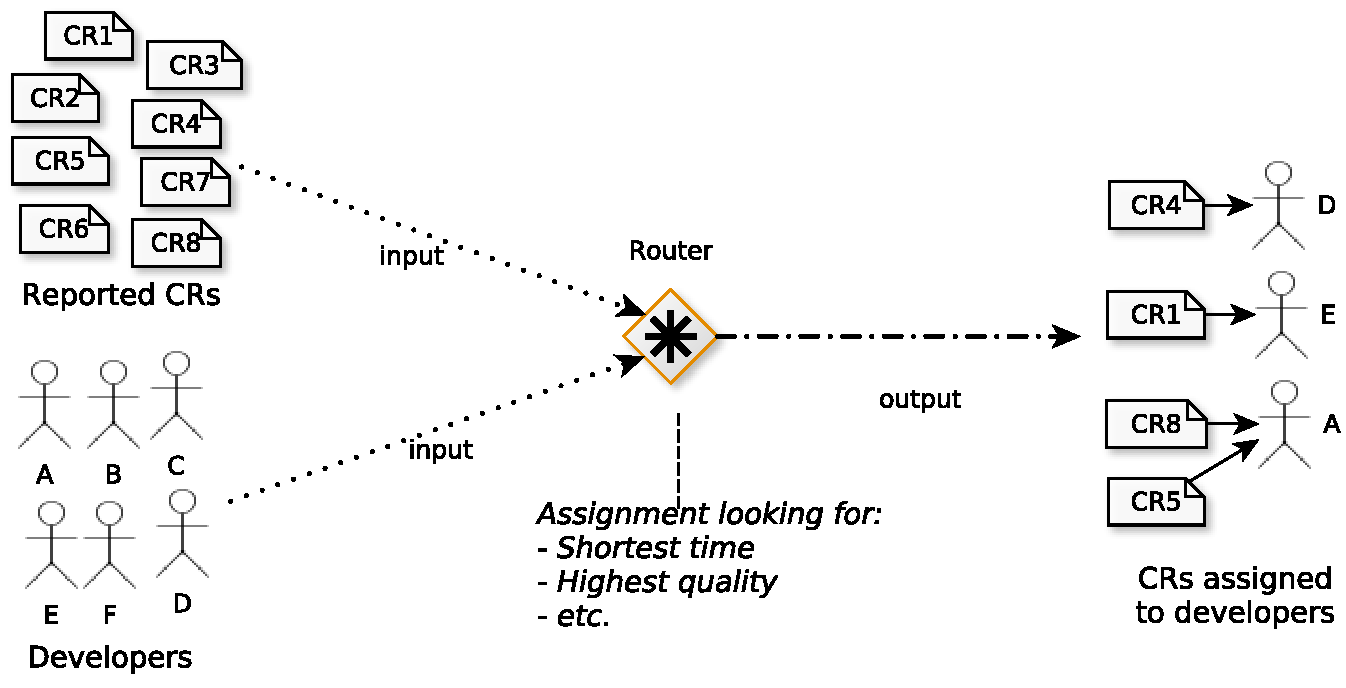
\includegraphics[width=\columnwidth]{images/assignment-schema.pdf}
  \footnotesize{Source: Made by the author.}
  \label{fig:assignment-schema}
\end{figure}

\lipsum[2-4]

Nevertheless, by increasing the amount of reported \acp{cr} or the size of the
development team, it is visible that the router becomes overloaded and the
\ac{cr} assignment becomes an intensive, error prone activity. It was confirmed
by \citet{Jeong2009}, which identified that 37\%-44\% of the \acp{cr} in Mozilla
and Eclipse projects did not reach the right developer in the first assignment.
These \acp{cr}, in turn, had their fixing time delayed because they needed to be
reassigned one or more times. Furthermore, if the \acp{cr} are not fixed by the
appropriate developers, there is also the chance of introducing new defects
during the \acp{cr} fixing.

In this context, we believe that it is necessary to develop methods and tools to
automate the assignment of \acp{cr} and ensure that the \acp{cr} are being
assigned to the appropriate developers. With these methods and tools, we could
reduce the time needed to perform the assignments and, given that the
appropriate developers are actually being selected, the quality and time for the
\ac{cr} fixing are also improved.

\section{Problem Statement}
\label{sec:intro-problem-statement}

As previously mentioned, software maintenance has been considered as the most
costly aspect of software development~\citep{swebok2004}. There is a myriad of
reasons for this situation. One of them is the many changes that are required
after software delivery due to poor documented and misunderstood requirements,
or simply because \emph{``the clients do not know what they
want''}~\citep{Brooks1995}.

Another reason is the fact that a set of development activities must be
inevitably performed in order to implement a change. For instance, for each
change to be implemented it is necessary to comprehend the existing software
artifacts, modify the software's source code to implement the change, perform
tests and verification, and deliver the new version of the software.
Additionally, very often, the implementation of the change ends up by
introducing new defects in the software.
   
A third reason is the management aspects of software maintenance. It is
necessary to keep track of all these changes that are performed, generally
considering different versions of the software and customers.

\lipsum[3-5]

\begin{enumerate}
  \item Firstly, the approaches available in the literature were designed to
  perform autonomously. That is, the software analysts do not have the control
  of the approach; they cannot modify the approach's behavior. Without
  such control, in turn, the approach cannot be properly calibrated. As a
  consequence, if the approach's performance is not satisfactory, it is simply
  discarded.
  \item Secondly, the reported values for accuracy of these approaches are
  still low. With low accuracy, the previous reason takes place. That is, as the
  approaches perform with low accuracy, and the software analysts do not have
  control over them, the approaches are simply discarded.
  \item Finally, the third reason concerns the lack of contextual information in
  those approaches. As is well known, software development companies are
  dynamic: developers move from projects; developers are hired/fired;
  developers enter in vacation or take a day off; and developers have different
  experiences. This dynamic influences the assignment of \acp{cr}. Thus,
  contextual information is a necessity in automated approaches.
\end{enumerate}

Based on this context, the main research question investigated by this thesis is:

\begin{description}
  \item[Research question] \emph{Is it possible to develop a new approach for
  automated \ac{cr} assignment with satisfactory accuracy, leveraging
  contextual information, and designed in order to put the software analysts in
  control of such approach?}
\end{description}

With the objective to answer this question, it is necessary to understand
current approaches available in the literature, choose the correct technologies
that could support dynamic environments and, mainly, understand the necessities
of software analysts regarding a new approach for automated \ac{cr} assignment.
Thus, the goal of the work described in this thesis can be stated as:

\begin{description}
  \item[Research objective] \emph{This work proposes an automated approach for
  \ac{cr} assignment which uses \ac{ir} models, expert systems, and
  context-aware information in order to select the appropriate developers. The
  approach is supported by the state-of-the-art in the management of \acp{cr} as
  well as by the understanding of the aspects concerning the \ac{cr} assignment
  activity itself.}
\end{description} 

\section{Overview of the Proposal}
\lipsum[1-5]

\section{Research Methodology}

This research design of this thesis is based on a multimethod
approach~\citep{Hesse-Biber2010}. Such approach combines two or more
quantitative (or qualitative) methods in a single study, such as a survey and an
experiment~\citep{Hesse-Biber2010}. Multimethod must not be confused with mixed
method. In this last, methods for both qualitative and quantitative types of
research are applied in a single study. On the other hand, multimethod studies
combine different methods for a single research type.

When applying a multimethod approach, the triangulation is used to consolidate
the results from the different methods, considering, however, that the same
research question(s) was/were investigated in these methods. As a consequence,
the triangulation of methods enhances the conclusions and completeness of the
study, bringing more credibility to the research
findings~\citep{Hesse-Biber2010}. \figref{fig:research-methodology-thesis} shows
the multimethod research design applied in this thesis.

\begin{figure}[h]
\centering
  \caption[Research methodology.]{The research methodology applied for this
  thesis.}
  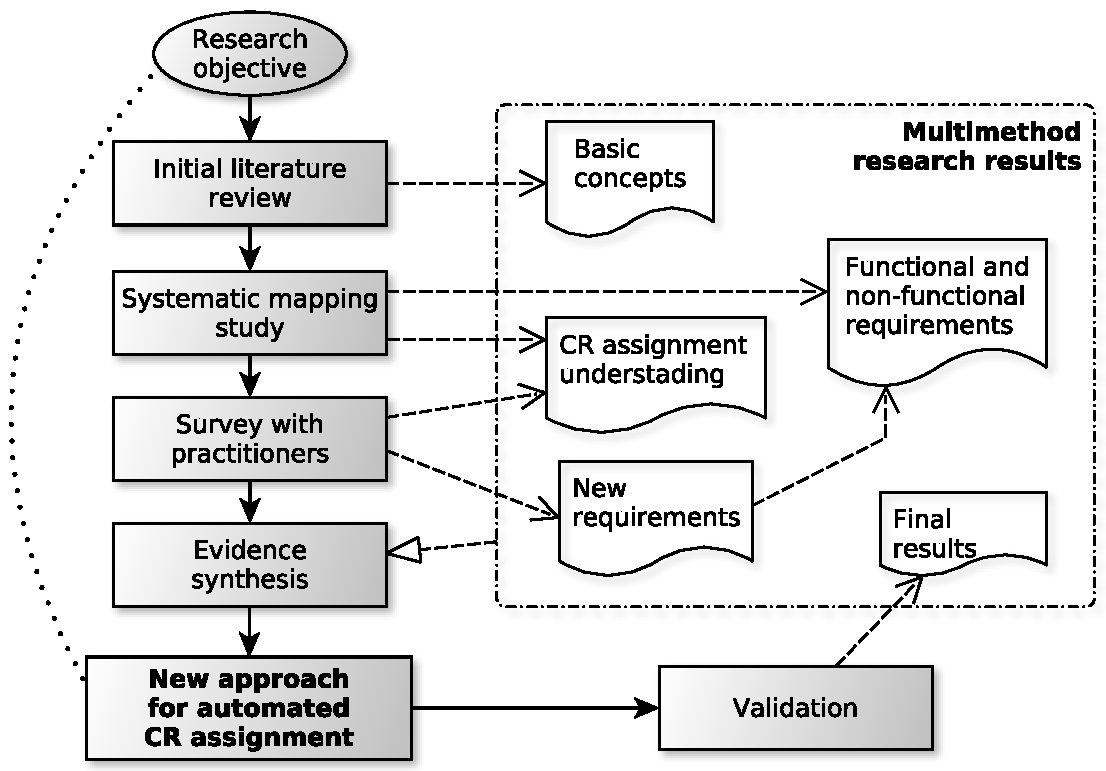
\includegraphics[width=\columnwidth]{images/research-methodology-thesis.pdf}
  \footnotesize{Source: Made by the author.}
  \label{fig:research-methodology-thesis}
\end{figure}

The design started by stating the research objective, which we defined in
\secref{sec:intro-problem-statement}, and performing the initial literature
review. This last provided the basic concepts and understanding of the area.
Then, a systematic mapping study and a questionnaire-based survey were
conducted. These two gathered detailed information on our research topic.
Indeed, both of them were used to understand the key aspects of \ac{cr}
assignment and identify the set of requirements to automate the assignments. In
the evidence synthesis step, these results were detailed and organized in order
to formulate the approach to automate \ac{cr} assignments, which was constructed
in the next step. Finally, the research design states the validation of the
proposed approach.

\section{Out of Scope}

As the proposed approach is part of a broader context, a set of related aspects
will be left out of its scope. Thus, the following topics are not directly
addressed in this thesis:

\begin{enumerate}
  \item \textbf{Tools for \ac{cr} management.} We are addressing
  a specific aspect of \ac{cr} management, which is the \ac{cr} assignment
  activity. Thus, it is out of scope of this thesis to provide a
  complete solution for \ac{cr} management. Instead, we are planning to
  implement standalone software which will be able to integrate with the
  most well known tools for \ac{cr} management, such as Mantis, Bugzilla, and
  Trac, providing a service to leverage the automation of \ac{cr}
  assignments.
  
  \item \textbf{Software maintenance process.} Software maintenance involves
  a set of activities aiming at implementing modifications in some software
  project. These activities must be coordinated through a process so that the
  maintenance can be successful. In Chapter 2, we discuss some of
  these processes. However, in this thesis, we are not concerned with the
  maintenance process itself. Actually, it should be transparent in our approach
  to automate \ac{cr} assignment. Thus, it is out of scope of this
  thesis to provide any process assessment for software maintenance beyond the
  activity of \ac{cr} assignment.
  
  \item \textbf{\ac{ir} models.} Many models for \ac{ir} have been proposed for
  different objectives, including the \ac{cr} assignment itself. However, due to
  the broad availability of these models, it is out of scope of this thesis to
  develop a new one. Instead, the \ac{ir} models with better performance,
  identified through the systematic mapping study, were chose to be
  integrated in our approach;
  
  \item \textbf{Rule-based expert systems.} Similar to \ac{ir} models,
  rule-based expert systems have a long history of development. Thus, our
  approach does not intend to develop a whole new system with this purpose.
  Actually, we integrated in our approach the
  Drools\footnote{\url{http://www.jboss.org/drools/}} expert system, which is a
  mature tool that can be easily manipulated;
  
  \item \textbf{Mathematical formulations on NP-Complete problems.} We
  understand that the problem of assigning \acp{cr} to software developers is in
  the broad category of \emph{assignment problems}, which is well known to be
  NP-Complete. Thus, could be formulated as such. However, the mathematical
  formulations of the \ac{cr} assignment problem is out of scope of this thesis.
  As well as finding an optimal solution on the context of NP-Complete problems
  is also out of scope. The main reason for this is the human factors and
  context variables that are involved in the assignment of \acp{cr}, which
  make this problem hard to be computable. A mathematical formulation of the
  \ac{cr} assignment problem is provided by~\citet{Rahman2009}.
\end{enumerate}

\section{Statement of the Contributions}
\lipsum[6-7]

\begin{enumerate}
  \item An overview of the software maintenance concepts and processes, with
  emphasis on the importance of \ac{cr} management aspects; 
  \item A survey performed with practitioners from a large organization, in
  order to understand the aspects of the \ac{cr} assignment
  activity. Published in the \emph{17$^{th}$ International Conference on Evaluation
  and Assessment in Software Engineering (EASE'2013)}~\citep{CavalcantiEASE2013};
  \item A replication of the previous survey in two more organizations;
  \item A systematic mapping study performed to understand the challenges and
  opportunities of \ac{cr} management, as well as to identify research gaps and
  the road ahead. Accepted for publication in the
  \emph{Journal of Software: Evolution and Process}~\citep{CavalcantiJSEP2013};
  \item The definition of the functional and non-functional requirements that
  are required to effectively automate \ac{cr} assignment, which takes as input
  the systematic mapping study and the survey;
  \item The definition of an approach that satisfies the
  identified requirements to automate the \ac{cr} assignment activity;
  \item The realization of the proposed approach's architecture, in which we
  described the methods and techniques used for the implementation, as well as the
  components that have to be built and the third party components that should be
  assembled together in order to provide a service for automated \ac{cr}
  assignment; and
  \item The evaluation of the proposed approach, performed as an offline
  experiment simulating a real context.
\end{enumerate}

\section{Organization of the Thesis}

\lipsum[5-10]

%\chapter{Background}

\section{Introduction}

\lipsum[1-4]

\section{Section}

\lipsum[2-4]

\subsection{Subsection}

\lipsum[2-4]
%\section{Objects of Analysis}
\label{sec:subjects}

%% We evaluated the characteristics of test suites in open-source
%% development from a sample set of Java projects from \github{}.  We are
%% interested to evaluate non-trivial test suites from popular projects
%% that are in activity.

%% , which is used on
%% \github{} to indicate appreciation of a user to a
%% project~\cite{github-stars},

We used \github{}'s search API~\cite{githubsearch} to identify
projects that satisfy the following criteria: (1) the primary language
is Java\footnote{In case of projects in multiple languages, the
  \github{} API considers the predominant language as the primary
  language.}, (2) the project has at least 100 stars, (3) the latest
update was on or after January 1st, 2016, and (4) the \emph{readme}
file contains the string \emph{mvn}.  We focused on Java for its
popularity.  Although there is no clearcut limit on the number of
\github{} stars~\cite{github-stars} to define relevant projects, we
observed that 100 was enough to eliminate trivial subjects. The third
criteria serves to skip projects without recent activity. The fourth
criteria is an approximation to find Maven projects.\Comment{ The
  rationale is that if the string \emph{mvn} exists in the
  \emph{readme} file, it may represent a Maven call (\eg, to compile
  or to test the project).} We focused on Maven for its popularity on
Java projects.  Important to highlight that, as of now, the
\github{}'s search API can only reflect contents from README file (not
other code elements); it does not provide a feature to search for
projects containing certain files in the dir structure (\eg{},
\emph{pom.xml}).  Figure~\ref{fig:subject-query} illustrates the query
to the \github{} API as an HTTP request.  

\vspace{1ex}
\begin{figure}[h!]
\centering
\scriptsize
\lstset{
    escapeinside={@}{@},
    numbers=left,xleftmargin=1em,frame=single,framexleftmargin=0.5em,
    basicstyle=\ttfamily\scriptsize, boxpos=c, numberstyle=\tiny,
    deletekeywords={true}
}
\begin{lstlisting}
https://api.github.com/search/repositories?q=language:java
        +stars:>=100+pushed:>=2016-01-01
        +mvn%20in:readme+sort:stars
\end{lstlisting}
    \caption{\label{fig:subject-query} Query to the \github{} API for
    projects with the following criteria: (1) Java, (2) at least 100
    stars, (3) updated on January 1st, 2016 (or later), (4) contains
    the string \emph{mvn} in the \emph{readme} file. Output is
    paginated in descending order of stars.}
\end{figure}

After obtaining a list of potential projects, we filtered those
containing a \pomf{} file in the root directory.  A Maven project may
contain several sub-modules with multiple \pomf{} files.\Comment{  We
based our methodology to select experimental subjects on other recent
studies in testing and
debugging~\cite{gligoric-etal-issta2015,perez-etal-icst2017}.} As of
March 25th 2017, our search criteria returned \SubjectsGithub{}
subjects. Figure~\ref{fig:subjects} summarizes our sample set. 

\begin{figure}[ht]
    \centering
    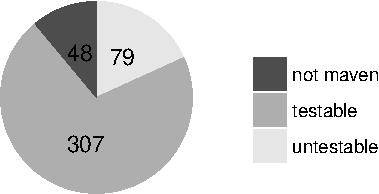
\includegraphics[width=0.25\textwidth]{plots/subjs.pdf}
    \caption{\label{fig:subjects}We fetched \SubjectsGithub{} popular projects
    hosted on \github{}. From this initial sample, we ignored
    \SubjectsGithubNotMaven{} projects without Maven support,
    \SubjectsGithubNotCompilable{} were unable to compile, and
    \SubjectsGithubNotTestable{} untestable projects\Comment{, and
    \SubjectsGithubFlaky{} projects with flaky tests}. We considered
    \numSubjs{} projects to conduct our study.}
\end{figure}

From \SubjectsGithub{} downloaded projects, \SubjectsGithubNotMaven{}
projects were not Maven or did not have a \pomf{} in the root
directory, \SubjectsGithubNotCompilable{} were unable to compile due
to missing dependencies, and \SubjectsGithubNotTestable{} projects
were untestable due to incompatible testing environment.  We also
found \SubjectsGithubFlaky{} projects with ``flaky'' tests.  We
considered those projects but ignored their tests (using JUnit's
\CodeIn{@Ignore} annotation) as to avoid measurement noise.  To detect
those projects, we executed every test suite for three times.  Our
final set of subjects consists of \numSubjs{} projects.

\subsection{Setup and Replication}
\label{sec:setup}

To run our experiments, we used a Core i7-4790 (3.60 GHz) Intel
processor machine with eight virtual CPUs (four cores with two native
threads each) and 16GB of memory, running Ubuntu 14.04 LTS Trusty Tahr
(64-bit version).  Software settings include \Comment{the Linux
  \emph{sysstat} package to measure performance, }git to fetch
subjects, Java 8, and Maven 3.3.9 to build and test subjects. We used
Python\Comment{ 3.4}, Bash, R and Ruby\Comment{ 2.3} to process the
data and generate plots.  All source artifacts are publicly available
for replication (on request)\Comment{ at \Fix{create gh-pages}}.  This
includes supporting scripts (\eg, the script that test subjects and
generates raw analysis data) and the full list of projects. \Comment{,
  and a \emph{Vagrantfile} to emulate our hardware and all software
  dependencies.}


\section{Evaluation}
\label{sec:eval}

%% We are interested in understanding the prevalence of time-consuming
%% test suites and main sources of execution cost. We want to understand
%% how the execution cost is distributed on test cases within a test
%% suite and how developers approach test execution. Based on that, we
%% study parallelization of testing frameworks and build systems.  More
%% precisely, we investigate how prevalent test parallelization is, the
%% potential for improving execution cost, issues of flakiness that
%% hinders the use of parallelization, and how to address those issues.
%% More specifically, we pose the following research questions:

%% The first research question addresses the prevalence of long-running
%% test suites. We are interested to know if costly test suites are
%% common in open-source projects.  The second research question
%% addresses the relationship of test cases and the overall execution
%% cost: we are interested to investigate how the execution time is
%% distributed among test cases.  In the third research question, we
%% investigate if developers consider low-level parallelism features
%% available out-of-the-box to amortize test execution (see
%% Section~\ref{sec:modes}). In addition, we want to identify what
%% configurations are often used and why they are more popular (if any).
%% The fourth research question addresses the impact of low-level
%% parallelism on test execution from projects in our sample set. We want
%% to identify subjects that already use test parallelization and compare
%% their performance in contrast to sequential execution. In addition, we
%% are interested in evaluating the performance of sequential test suites
%% with different parallelization settings.
%% Finally, the fifth research question discusses the limitations and
%% insights to overcome the pitfalls of parallelization.

%% \Comment{
%%     \Fix{distribution of execution time per test case. For each subject
%%     identified in the first research question, we investigate how
%%     balanced is the cost of the test suite in contrast to the cost of
%%     test cases and if there are subjects where the time cost is mostly
%%     dominated by a small fraction of test cases.} \Fix{The third research
%%     question addresses the distribution of regression tests according
%%     to the use of computational resources.  We are interested in
%%     investigating if regression test suites are CPU intensive and if there
%%     are opportunities to improve performance. The RQ4 addresses}
%%     \Fix{...elaborate...}

%%     The rationale is that if the time cost of a regression test is equally
%%     distributed among test cases, the execution cost could be potentially
%%     improved by running tests in parallel (in contrast to the scenario
%%     where only one test case dominates most of the execution time).
%% }

We pose the following research questions, organized by the dimensions
of analysis we presented in Section~\ref{sec:intro}.


%% Feasibility
\newcommand{\numRQFeasibilityOne}{RQ1}
\newcommand{\RQFeasibilityOne}{How prevalent is the occurence of time-consuming
  test suites\Comment{ in open-source projects}?}

\newcommand{\numRQFeasibilityTwo}{RQ2}
\newcommand{\RQFeasibilityTwo}{How time is distributed across test cases?}

%% Adoption
\newcommand{\numRQAdoptionOne}{RQ3}
\newcommand{\RQAdoptionOne}{How popular is test suite
  parallelization\Comment{ in open-source projects}?}

\newcommand{\numRQAdoptionTwo}{RQ4}
\newcommand{\RQAdoptionTwo}{What are the main reasons that prevent developers
  from using test suite parallelization?}

%% Speedups
\newcommand{\numRQSpeedupOne}{RQ5}
\newcommand{\RQSpeedupOne}{What are the speedups obtained with parallelization
  (in projects that actually use it)?}

\newcommand{\numRQSpeedupTwo}{RQ6}
\newcommand{\RQSpeedupTwo}{How test execution scales with the number of
  available CPUs?}

%% Issues
\newcommand{\numRQIssuesOne}{RQ7}
\newcommand{\RQIssuesOne}{How parallel execution configurations affect testing
  costs and flakiness?}


\setlist[itemize]{leftmargin=1em}
\begin{itemize}
\item Feasibility
  \begin{itemize}
  \item \textbf{\numRQFeasibilityOne.} \RQFeasibilityOne
  \item \textbf{\numRQFeasibilityTwo.} \RQFeasibilityTwo    
  \end{itemize}
\item Adoption
  \begin{itemize}
  \item \textbf{\numRQAdoptionOne.} \RQAdoptionOne    
  \item \textbf{\numRQAdoptionTwo.} \RQAdoptionTwo
  \end{itemize}
\item Speedups
  \begin{itemize}
  \item \textbf{\numRQSpeedupOne.} \RQSpeedupOne
  \item \textbf{\numRQSpeedupTwo.} \RQSpeedupTwo
  \end{itemize}      
\item Issues
  \begin{itemize}
  \item \textbf{\numRQIssuesOne.} \RQIssuesOne    
  \end{itemize}
\end{itemize}

%%\newcommand{\RQFeasibilityTwo}{What is the distribution of CPU and IO bound
%%regression test suites from the sample set?}
%%
%%\newcommand{\RQAdoptionOne}{How uniformly distributed is the execution time
%%across test cases in costly projects?}
%%
%%\newcommand{\RQAdoptionTwo}{How often developers use the parallelism features
%%from build systems to improve runtime performance?}



\subsection{Feasibility}
\label{sec:rqA}
\label{sec:rqB}

\begin{itemize}
    \item \numRQFeasibilityOne{}. \textbf{\RQFeasibilityOne}
\end{itemize}
%\Jbc{The following steps may change $\rightarrow$}

To evaluate prevalence of projects with costly test suites, we
considered the \numSubjs{} testable subjects from
Figure~\ref{fig:subjects}.  Figure~\ref{fig:mvn-execution} illustrates
the script we used to measure time.

We took the following actions to isolate our environment from
measurement noise.  First, we observed that some test tasks called
test-unrelated tasks (\eg, \emph{javadoc} generation and static
analyses) that could interfere in our time measurements.  To address
that potential issue, we inspected Maven execution logs from a sample
including a hundred projects prior to running the script from
Figure~\ref{fig:mvn-execution}.  The tasks we found were ignored from
execution (lines 1-3).  Furthermore, to avoid noise from operating
system events, we configured our workstation to run only essential
services.  The machine was dedicated to our experiments and we
accessed it via SSH. In addition, we configured the \CodeIn{isolcpus}
option from the Linux Kernel \cite{linux-kernel} to isolate six
virtual CPUs to run our experiments, leaving the remaining CPUs to run
OS processes~\cite{isolcpus-use}.  The rationale for this decision is
to prevent context-switching between user processes (running the
experiment) and OS-related processes.  Finally, to make sure our
measurements were fair, we compared timings corresponding to the
sequential execution of tests using Maven with that obtained with
JUnit's default \CodeIn{JUnitCore} runner, invoked from the command
line.  Results were very close.

The main loop (lines 5-11) of the script in
Figure~\ref{fig:mvn-execution} iterates over the list of subjects and
invokes Maven multiple times\Comment{ to isolate cost of running
  tests} (lines 7-9).  It first compiles the source and test files
(line 7), make all dependencies available locally (line 8), and then
runs the tests in offline mode as to skip the package update task,
enabled by default (line 9). After execution, we used a regular
expression on the output log to extract elapsed time (line 10).

%% We executed each project's test suite for
%% \Fix{5} times through Maven and directly through JUnit each project

\section{Objects of Analysis}
\label{sec:subjects}

%% We evaluated the characteristics of test suites in open-source
%% development from a sample set of Java projects from \github{}.  We are
%% interested to evaluate non-trivial test suites from popular projects
%% that are in activity.

%% , which is used on
%% \github{} to indicate appreciation of a user to a
%% project~\cite{github-stars},

We used \github{}'s search API~\cite{githubsearch} to identify
projects that satisfy the following criteria: (1) the primary language
is Java\footnote{In case of projects in multiple languages, the
  \github{} API considers the predominant language as the primary
  language.}, (2) the project has at least 100 stars, (3) the latest
update was on or after January 1st, 2016, and (4) the \emph{readme}
file contains the string \emph{mvn}.  We focused on Java for its
popularity.  Although there is no clearcut limit on the number of
\github{} stars~\cite{github-stars} to define relevant projects, we
observed that 100 was enough to eliminate trivial subjects. The third
criteria serves to skip projects without recent activity. The fourth
criteria is an approximation to find Maven projects.\Comment{ The
  rationale is that if the string \emph{mvn} exists in the
  \emph{readme} file, it may represent a Maven call (\eg, to compile
  or to test the project).} We focused on Maven for its popularity on
Java projects.  Important to highlight that, as of now, the
\github{}'s search API can only reflect contents from README file (not
other code elements); it does not provide a feature to search for
projects containing certain files in the dir structure (\eg{},
\emph{pom.xml}).  Figure~\ref{fig:subject-query} illustrates the query
to the \github{} API as an HTTP request.  

\vspace{1ex}
\begin{figure}[h!]
\centering
\scriptsize
\lstset{
    escapeinside={@}{@},
    numbers=left,xleftmargin=1em,frame=single,framexleftmargin=0.5em,
    basicstyle=\ttfamily\scriptsize, boxpos=c, numberstyle=\tiny,
    deletekeywords={true}
}
\begin{lstlisting}
https://api.github.com/search/repositories?q=language:java
        +stars:>=100+pushed:>=2016-01-01
        +mvn%20in:readme+sort:stars
\end{lstlisting}
    \caption{\label{fig:subject-query} Query to the \github{} API for
    projects with the following criteria: (1) Java, (2) at least 100
    stars, (3) updated on January 1st, 2016 (or later), (4) contains
    the string \emph{mvn} in the \emph{readme} file. Output is
    paginated in descending order of stars.}
\end{figure}

After obtaining a list of potential projects, we filtered those
containing a \pomf{} file in the root directory.  A Maven project may
contain several sub-modules with multiple \pomf{} files.\Comment{  We
based our methodology to select experimental subjects on other recent
studies in testing and
debugging~\cite{gligoric-etal-issta2015,perez-etal-icst2017}.} As of
March 25th 2017, our search criteria returned \SubjectsGithub{}
subjects. Figure~\ref{fig:subjects} summarizes our sample set. 

\begin{figure}[ht]
    \centering
    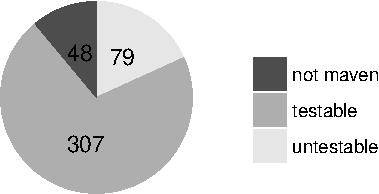
\includegraphics[width=0.25\textwidth]{plots/subjs.pdf}
    \caption{\label{fig:subjects}We fetched \SubjectsGithub{} popular projects
    hosted on \github{}. From this initial sample, we ignored
    \SubjectsGithubNotMaven{} projects without Maven support,
    \SubjectsGithubNotCompilable{} were unable to compile, and
    \SubjectsGithubNotTestable{} untestable projects\Comment{, and
    \SubjectsGithubFlaky{} projects with flaky tests}. We considered
    \numSubjs{} projects to conduct our study.}
\end{figure}

From \SubjectsGithub{} downloaded projects, \SubjectsGithubNotMaven{}
projects were not Maven or did not have a \pomf{} in the root
directory, \SubjectsGithubNotCompilable{} were unable to compile due
to missing dependencies, and \SubjectsGithubNotTestable{} projects
were untestable due to incompatible testing environment.  We also
found \SubjectsGithubFlaky{} projects with ``flaky'' tests.  We
considered those projects but ignored their tests (using JUnit's
\CodeIn{@Ignore} annotation) as to avoid measurement noise.  To detect
those projects, we executed every test suite for three times.  Our
final set of subjects consists of \numSubjs{} projects.

\subsection{Setup and Replication}
\label{sec:setup}

To run our experiments, we used a Core i7-4790 (3.60 GHz) Intel
processor machine with eight virtual CPUs (four cores with two native
threads each) and 16GB of memory, running Ubuntu 14.04 LTS Trusty Tahr
(64-bit version).  Software settings include \Comment{the Linux
  \emph{sysstat} package to measure performance, }git to fetch
subjects, Java 8, and Maven 3.3.9 to build and test subjects. We used
Python\Comment{ 3.4}, Bash, R and Ruby\Comment{ 2.3} to process the
data and generate plots.  All source artifacts are publicly available
for replication (on request)\Comment{ at \Fix{create gh-pages}}.  This
includes supporting scripts (\eg, the script that test subjects and
generates raw analysis data) and the full list of projects. \Comment{,
  and a \emph{Vagrantfile} to emulate our hardware and all software
  dependencies.}


\section{Evaluation}
\label{sec:eval}

%% We are interested in understanding the prevalence of time-consuming
%% test suites and main sources of execution cost. We want to understand
%% how the execution cost is distributed on test cases within a test
%% suite and how developers approach test execution. Based on that, we
%% study parallelization of testing frameworks and build systems.  More
%% precisely, we investigate how prevalent test parallelization is, the
%% potential for improving execution cost, issues of flakiness that
%% hinders the use of parallelization, and how to address those issues.
%% More specifically, we pose the following research questions:

%% The first research question addresses the prevalence of long-running
%% test suites. We are interested to know if costly test suites are
%% common in open-source projects.  The second research question
%% addresses the relationship of test cases and the overall execution
%% cost: we are interested to investigate how the execution time is
%% distributed among test cases.  In the third research question, we
%% investigate if developers consider low-level parallelism features
%% available out-of-the-box to amortize test execution (see
%% Section~\ref{sec:modes}). In addition, we want to identify what
%% configurations are often used and why they are more popular (if any).
%% The fourth research question addresses the impact of low-level
%% parallelism on test execution from projects in our sample set. We want
%% to identify subjects that already use test parallelization and compare
%% their performance in contrast to sequential execution. In addition, we
%% are interested in evaluating the performance of sequential test suites
%% with different parallelization settings.
%% Finally, the fifth research question discusses the limitations and
%% insights to overcome the pitfalls of parallelization.

%% \Comment{
%%     \Fix{distribution of execution time per test case. For each subject
%%     identified in the first research question, we investigate how
%%     balanced is the cost of the test suite in contrast to the cost of
%%     test cases and if there are subjects where the time cost is mostly
%%     dominated by a small fraction of test cases.} \Fix{The third research
%%     question addresses the distribution of regression tests according
%%     to the use of computational resources.  We are interested in
%%     investigating if regression test suites are CPU intensive and if there
%%     are opportunities to improve performance. The RQ4 addresses}
%%     \Fix{...elaborate...}

%%     The rationale is that if the time cost of a regression test is equally
%%     distributed among test cases, the execution cost could be potentially
%%     improved by running tests in parallel (in contrast to the scenario
%%     where only one test case dominates most of the execution time).
%% }

We pose the following research questions, organized by the dimensions
of analysis we presented in Section~\ref{sec:intro}.


%% Feasibility
\newcommand{\numRQFeasibilityOne}{RQ1}
\newcommand{\RQFeasibilityOne}{How prevalent is the occurence of time-consuming
  test suites\Comment{ in open-source projects}?}

\newcommand{\numRQFeasibilityTwo}{RQ2}
\newcommand{\RQFeasibilityTwo}{How time is distributed across test cases?}

%% Adoption
\newcommand{\numRQAdoptionOne}{RQ3}
\newcommand{\RQAdoptionOne}{How popular is test suite
  parallelization\Comment{ in open-source projects}?}

\newcommand{\numRQAdoptionTwo}{RQ4}
\newcommand{\RQAdoptionTwo}{What are the main reasons that prevent developers
  from using test suite parallelization?}

%% Speedups
\newcommand{\numRQSpeedupOne}{RQ5}
\newcommand{\RQSpeedupOne}{What are the speedups obtained with parallelization
  (in projects that actually use it)?}

\newcommand{\numRQSpeedupTwo}{RQ6}
\newcommand{\RQSpeedupTwo}{How test execution scales with the number of
  available CPUs?}

%% Issues
\newcommand{\numRQIssuesOne}{RQ7}
\newcommand{\RQIssuesOne}{How parallel execution configurations affect testing
  costs and flakiness?}


\setlist[itemize]{leftmargin=1em}
\begin{itemize}
\item Feasibility
  \begin{itemize}
  \item \textbf{\numRQFeasibilityOne.} \RQFeasibilityOne
  \item \textbf{\numRQFeasibilityTwo.} \RQFeasibilityTwo    
  \end{itemize}
\item Adoption
  \begin{itemize}
  \item \textbf{\numRQAdoptionOne.} \RQAdoptionOne    
  \item \textbf{\numRQAdoptionTwo.} \RQAdoptionTwo
  \end{itemize}
\item Speedups
  \begin{itemize}
  \item \textbf{\numRQSpeedupOne.} \RQSpeedupOne
  \item \textbf{\numRQSpeedupTwo.} \RQSpeedupTwo
  \end{itemize}      
\item Issues
  \begin{itemize}
  \item \textbf{\numRQIssuesOne.} \RQIssuesOne    
  \end{itemize}
\end{itemize}

%%\newcommand{\RQFeasibilityTwo}{What is the distribution of CPU and IO bound
%%regression test suites from the sample set?}
%%
%%\newcommand{\RQAdoptionOne}{How uniformly distributed is the execution time
%%across test cases in costly projects?}
%%
%%\newcommand{\RQAdoptionTwo}{How often developers use the parallelism features
%%from build systems to improve runtime performance?}



\subsection{Feasibility}
\label{sec:rqA}
\label{sec:rqB}

\begin{itemize}
    \item \numRQFeasibilityOne{}. \textbf{\RQFeasibilityOne}
\end{itemize}
%\Jbc{The following steps may change $\rightarrow$}

To evaluate prevalence of projects with costly test suites, we
considered the \numSubjs{} testable subjects from
Figure~\ref{fig:subjects}.  Figure~\ref{fig:mvn-execution} illustrates
the script we used to measure time.

We took the following actions to isolate our environment from
measurement noise.  First, we observed that some test tasks called
test-unrelated tasks (\eg, \emph{javadoc} generation and static
analyses) that could interfere in our time measurements.  To address
that potential issue, we inspected Maven execution logs from a sample
including a hundred projects prior to running the script from
Figure~\ref{fig:mvn-execution}.  The tasks we found were ignored from
execution (lines 1-3).  Furthermore, to avoid noise from operating
system events, we configured our workstation to run only essential
services.  The machine was dedicated to our experiments and we
accessed it via SSH. In addition, we configured the \CodeIn{isolcpus}
option from the Linux Kernel \cite{linux-kernel} to isolate six
virtual CPUs to run our experiments, leaving the remaining CPUs to run
OS processes~\cite{isolcpus-use}.  The rationale for this decision is
to prevent context-switching between user processes (running the
experiment) and OS-related processes.  Finally, to make sure our
measurements were fair, we compared timings corresponding to the
sequential execution of tests using Maven with that obtained with
JUnit's default \CodeIn{JUnitCore} runner, invoked from the command
line.  Results were very close.

The main loop (lines 5-11) of the script in
Figure~\ref{fig:mvn-execution} iterates over the list of subjects and
invokes Maven multiple times\Comment{ to isolate cost of running
  tests} (lines 7-9).  It first compiles the source and test files
(line 7), make all dependencies available locally (line 8), and then
runs the tests in offline mode as to skip the package update task,
enabled by default (line 9). After execution, we used a regular
expression on the output log to extract elapsed time (line 10).

%% We executed each project's test suite for
%% \Fix{5} times through Maven and directly through JUnit each project

\section{Objects of Analysis}
\label{sec:subjects}

%% We evaluated the characteristics of test suites in open-source
%% development from a sample set of Java projects from \github{}.  We are
%% interested to evaluate non-trivial test suites from popular projects
%% that are in activity.

%% , which is used on
%% \github{} to indicate appreciation of a user to a
%% project~\cite{github-stars},

We used \github{}'s search API~\cite{githubsearch} to identify
projects that satisfy the following criteria: (1) the primary language
is Java\footnote{In case of projects in multiple languages, the
  \github{} API considers the predominant language as the primary
  language.}, (2) the project has at least 100 stars, (3) the latest
update was on or after January 1st, 2016, and (4) the \emph{readme}
file contains the string \emph{mvn}.  We focused on Java for its
popularity.  Although there is no clearcut limit on the number of
\github{} stars~\cite{github-stars} to define relevant projects, we
observed that 100 was enough to eliminate trivial subjects. The third
criteria serves to skip projects without recent activity. The fourth
criteria is an approximation to find Maven projects.\Comment{ The
  rationale is that if the string \emph{mvn} exists in the
  \emph{readme} file, it may represent a Maven call (\eg, to compile
  or to test the project).} We focused on Maven for its popularity on
Java projects.  Important to highlight that, as of now, the
\github{}'s search API can only reflect contents from README file (not
other code elements); it does not provide a feature to search for
projects containing certain files in the dir structure (\eg{},
\emph{pom.xml}).  Figure~\ref{fig:subject-query} illustrates the query
to the \github{} API as an HTTP request.  

\vspace{1ex}
\begin{figure}[h!]
\centering
\scriptsize
\lstset{
    escapeinside={@}{@},
    numbers=left,xleftmargin=1em,frame=single,framexleftmargin=0.5em,
    basicstyle=\ttfamily\scriptsize, boxpos=c, numberstyle=\tiny,
    deletekeywords={true}
}
\begin{lstlisting}
https://api.github.com/search/repositories?q=language:java
        +stars:>=100+pushed:>=2016-01-01
        +mvn%20in:readme+sort:stars
\end{lstlisting}
    \caption{\label{fig:subject-query} Query to the \github{} API for
    projects with the following criteria: (1) Java, (2) at least 100
    stars, (3) updated on January 1st, 2016 (or later), (4) contains
    the string \emph{mvn} in the \emph{readme} file. Output is
    paginated in descending order of stars.}
\end{figure}

After obtaining a list of potential projects, we filtered those
containing a \pomf{} file in the root directory.  A Maven project may
contain several sub-modules with multiple \pomf{} files.\Comment{  We
based our methodology to select experimental subjects on other recent
studies in testing and
debugging~\cite{gligoric-etal-issta2015,perez-etal-icst2017}.} As of
March 25th 2017, our search criteria returned \SubjectsGithub{}
subjects. Figure~\ref{fig:subjects} summarizes our sample set. 

\begin{figure}[ht]
    \centering
    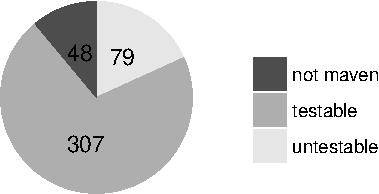
\includegraphics[width=0.25\textwidth]{plots/subjs.pdf}
    \caption{\label{fig:subjects}We fetched \SubjectsGithub{} popular projects
    hosted on \github{}. From this initial sample, we ignored
    \SubjectsGithubNotMaven{} projects without Maven support,
    \SubjectsGithubNotCompilable{} were unable to compile, and
    \SubjectsGithubNotTestable{} untestable projects\Comment{, and
    \SubjectsGithubFlaky{} projects with flaky tests}. We considered
    \numSubjs{} projects to conduct our study.}
\end{figure}

From \SubjectsGithub{} downloaded projects, \SubjectsGithubNotMaven{}
projects were not Maven or did not have a \pomf{} in the root
directory, \SubjectsGithubNotCompilable{} were unable to compile due
to missing dependencies, and \SubjectsGithubNotTestable{} projects
were untestable due to incompatible testing environment.  We also
found \SubjectsGithubFlaky{} projects with ``flaky'' tests.  We
considered those projects but ignored their tests (using JUnit's
\CodeIn{@Ignore} annotation) as to avoid measurement noise.  To detect
those projects, we executed every test suite for three times.  Our
final set of subjects consists of \numSubjs{} projects.

\subsection{Setup and Replication}
\label{sec:setup}

To run our experiments, we used a Core i7-4790 (3.60 GHz) Intel
processor machine with eight virtual CPUs (four cores with two native
threads each) and 16GB of memory, running Ubuntu 14.04 LTS Trusty Tahr
(64-bit version).  Software settings include \Comment{the Linux
  \emph{sysstat} package to measure performance, }git to fetch
subjects, Java 8, and Maven 3.3.9 to build and test subjects. We used
Python\Comment{ 3.4}, Bash, R and Ruby\Comment{ 2.3} to process the
data and generate plots.  All source artifacts are publicly available
for replication (on request)\Comment{ at \Fix{create gh-pages}}.  This
includes supporting scripts (\eg, the script that test subjects and
generates raw analysis data) and the full list of projects. \Comment{,
  and a \emph{Vagrantfile} to emulate our hardware and all software
  dependencies.}


\section{Evaluation}
\label{sec:eval}

%% We are interested in understanding the prevalence of time-consuming
%% test suites and main sources of execution cost. We want to understand
%% how the execution cost is distributed on test cases within a test
%% suite and how developers approach test execution. Based on that, we
%% study parallelization of testing frameworks and build systems.  More
%% precisely, we investigate how prevalent test parallelization is, the
%% potential for improving execution cost, issues of flakiness that
%% hinders the use of parallelization, and how to address those issues.
%% More specifically, we pose the following research questions:

%% The first research question addresses the prevalence of long-running
%% test suites. We are interested to know if costly test suites are
%% common in open-source projects.  The second research question
%% addresses the relationship of test cases and the overall execution
%% cost: we are interested to investigate how the execution time is
%% distributed among test cases.  In the third research question, we
%% investigate if developers consider low-level parallelism features
%% available out-of-the-box to amortize test execution (see
%% Section~\ref{sec:modes}). In addition, we want to identify what
%% configurations are often used and why they are more popular (if any).
%% The fourth research question addresses the impact of low-level
%% parallelism on test execution from projects in our sample set. We want
%% to identify subjects that already use test parallelization and compare
%% their performance in contrast to sequential execution. In addition, we
%% are interested in evaluating the performance of sequential test suites
%% with different parallelization settings.
%% Finally, the fifth research question discusses the limitations and
%% insights to overcome the pitfalls of parallelization.

%% \Comment{
%%     \Fix{distribution of execution time per test case. For each subject
%%     identified in the first research question, we investigate how
%%     balanced is the cost of the test suite in contrast to the cost of
%%     test cases and if there are subjects where the time cost is mostly
%%     dominated by a small fraction of test cases.} \Fix{The third research
%%     question addresses the distribution of regression tests according
%%     to the use of computational resources.  We are interested in
%%     investigating if regression test suites are CPU intensive and if there
%%     are opportunities to improve performance. The RQ4 addresses}
%%     \Fix{...elaborate...}

%%     The rationale is that if the time cost of a regression test is equally
%%     distributed among test cases, the execution cost could be potentially
%%     improved by running tests in parallel (in contrast to the scenario
%%     where only one test case dominates most of the execution time).
%% }

We pose the following research questions, organized by the dimensions
of analysis we presented in Section~\ref{sec:intro}.


%% Feasibility
\newcommand{\numRQFeasibilityOne}{RQ1}
\newcommand{\RQFeasibilityOne}{How prevalent is the occurence of time-consuming
  test suites\Comment{ in open-source projects}?}

\newcommand{\numRQFeasibilityTwo}{RQ2}
\newcommand{\RQFeasibilityTwo}{How time is distributed across test cases?}

%% Adoption
\newcommand{\numRQAdoptionOne}{RQ3}
\newcommand{\RQAdoptionOne}{How popular is test suite
  parallelization\Comment{ in open-source projects}?}

\newcommand{\numRQAdoptionTwo}{RQ4}
\newcommand{\RQAdoptionTwo}{What are the main reasons that prevent developers
  from using test suite parallelization?}

%% Speedups
\newcommand{\numRQSpeedupOne}{RQ5}
\newcommand{\RQSpeedupOne}{What are the speedups obtained with parallelization
  (in projects that actually use it)?}

\newcommand{\numRQSpeedupTwo}{RQ6}
\newcommand{\RQSpeedupTwo}{How test execution scales with the number of
  available CPUs?}

%% Issues
\newcommand{\numRQIssuesOne}{RQ7}
\newcommand{\RQIssuesOne}{How parallel execution configurations affect testing
  costs and flakiness?}


\setlist[itemize]{leftmargin=1em}
\begin{itemize}
\item Feasibility
  \begin{itemize}
  \item \textbf{\numRQFeasibilityOne.} \RQFeasibilityOne
  \item \textbf{\numRQFeasibilityTwo.} \RQFeasibilityTwo    
  \end{itemize}
\item Adoption
  \begin{itemize}
  \item \textbf{\numRQAdoptionOne.} \RQAdoptionOne    
  \item \textbf{\numRQAdoptionTwo.} \RQAdoptionTwo
  \end{itemize}
\item Speedups
  \begin{itemize}
  \item \textbf{\numRQSpeedupOne.} \RQSpeedupOne
  \item \textbf{\numRQSpeedupTwo.} \RQSpeedupTwo
  \end{itemize}      
\item Issues
  \begin{itemize}
  \item \textbf{\numRQIssuesOne.} \RQIssuesOne    
  \end{itemize}
\end{itemize}

%%\newcommand{\RQFeasibilityTwo}{What is the distribution of CPU and IO bound
%%regression test suites from the sample set?}
%%
%%\newcommand{\RQAdoptionOne}{How uniformly distributed is the execution time
%%across test cases in costly projects?}
%%
%%\newcommand{\RQAdoptionTwo}{How often developers use the parallelism features
%%from build systems to improve runtime performance?}



\subsection{Feasibility}
\label{sec:rqA}
\label{sec:rqB}

\begin{itemize}
    \item \numRQFeasibilityOne{}. \textbf{\RQFeasibilityOne}
\end{itemize}
%\Jbc{The following steps may change $\rightarrow$}

To evaluate prevalence of projects with costly test suites, we
considered the \numSubjs{} testable subjects from
Figure~\ref{fig:subjects}.  Figure~\ref{fig:mvn-execution} illustrates
the script we used to measure time.

We took the following actions to isolate our environment from
measurement noise.  First, we observed that some test tasks called
test-unrelated tasks (\eg, \emph{javadoc} generation and static
analyses) that could interfere in our time measurements.  To address
that potential issue, we inspected Maven execution logs from a sample
including a hundred projects prior to running the script from
Figure~\ref{fig:mvn-execution}.  The tasks we found were ignored from
execution (lines 1-3).  Furthermore, to avoid noise from operating
system events, we configured our workstation to run only essential
services.  The machine was dedicated to our experiments and we
accessed it via SSH. In addition, we configured the \CodeIn{isolcpus}
option from the Linux Kernel \cite{linux-kernel} to isolate six
virtual CPUs to run our experiments, leaving the remaining CPUs to run
OS processes~\cite{isolcpus-use}.  The rationale for this decision is
to prevent context-switching between user processes (running the
experiment) and OS-related processes.  Finally, to make sure our
measurements were fair, we compared timings corresponding to the
sequential execution of tests using Maven with that obtained with
JUnit's default \CodeIn{JUnitCore} runner, invoked from the command
line.  Results were very close.

The main loop (lines 5-11) of the script in
Figure~\ref{fig:mvn-execution} iterates over the list of subjects and
invokes Maven multiple times\Comment{ to isolate cost of running
  tests} (lines 7-9).  It first compiles the source and test files
(line 7), make all dependencies available locally (line 8), and then
runs the tests in offline mode as to skip the package update task,
enabled by default (line 9). After execution, we used a regular
expression on the output log to extract elapsed time (line 10).

%% We executed each project's test suite for
%% \Fix{5} times through Maven and directly through JUnit each project

\input{codes/evaluation}

We ran the test suite for each subject three times, reporting averaged
execution times in three ranges: tests that run within a minute
(\shortg{} group), tests that run in one to five minutes (\medg{}
group), and tests that run in five or more minutes (\longg{}
group). We followed a similar methodology to group projects by time as
Gligoric~\etal{}~\cite{gligoric-etal-issta2015} in their work on
regression test selection.\Comment{ and added the \medg{} group due to
  the variability of the time cost from subjects out of the \shortg{}
  group} Figure~\ref{fig:rq1-barplot} shows the number of projects in
each group.  As expected, \longg{} and \medg{} projects do not occur
as frequently as \shortg{} projects.  However, they do occur in
relatively high numbers.

Figure~\ref{fig:rq1-boxplot} shows cost distribution of test suites in
each group as boxplots.  Note that the y-ranges are different.  The
distribution associated with the \shortg{} group is the most
unbalanced (right skewed)\Comment{ with outliers closed to the \medg{}
  group}.  The test suites in this group ran in 15 or less seconds for
over 75\% of the cases.  Such scenarios constitute the majority of the
cases we analyzed.  Considering the groups \medg{} and \longg{},
however, we found many costly executions.  Nearly 75\% of the projects
from the \medg{} group take over 3.5 minutes to run and nearly 75\% of
the projects from the \longg{} group take $\sim$20 minutes to run.  We
found cases in the \longg{} group were execution takes over 50 minutes
to complete, as can be observed from the outliers (dots) in the plot.

%% the median from the
%% \medg{} group is nearly two minutes and most of the subjects run in
%% less than four minutes; most of the \longg{} group runs in less than
%% 25 minutes but has outliers that require more than 50 minutes to
%% execute.



\begin{figure}[ht]
    \centering
    \begin{subfigure}{0.182\textwidth}
        \centering
        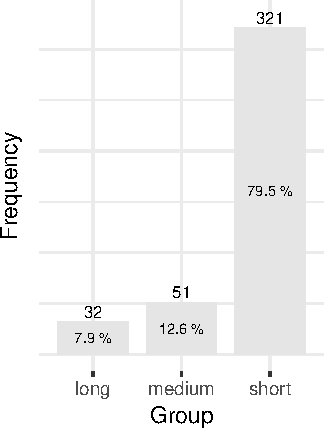
\includegraphics[width=\textwidth]{plots/barplot-timecost.pdf}
        \caption{\label{fig:rq1-barplot}}
    \end{subfigure}%
    ~
    \begin{subfigure}{0.25\textwidth}
        \centering
        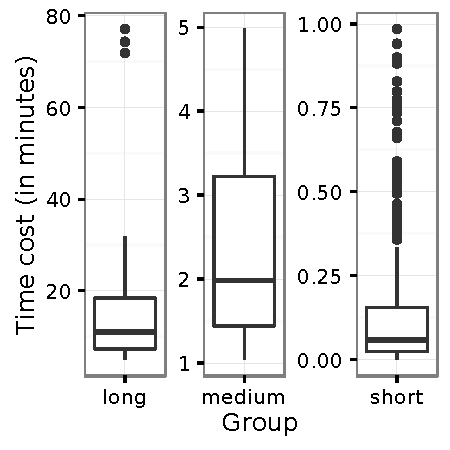
\includegraphics[width=\textwidth]{plots/boxplot-timecost.pdf}
        \caption{\label{fig:rq1-boxplot}}
    \end{subfigure}%
    \caption{(a) Subjects grouped by time cost ($t$): short run ($t <
    1m$), medium run ($1m \le t < 5m$), and long run ($5m \le t$); (b)
    Distribution of time cost by group.}
\end{figure}

%% Figure~\ref{fig:rq1-barplot} is a lower bound estimation of cost
%% because some tests may finish earlier than expected due to existing
%% test failures in the revision we downloaded.

It is important to note that we under-estimated cost in our
experiments for two main reasons.  First, some tests may finish
earlier than expected due to the observed test failures in some of the
revisions we downloaded.  From the \numSubjs{} testable projects,
\numSubjsPass{} successfully executed all tests and \numSubjsFail{}
reported some test failures.  Second, some projects may omit
long-running tests on their default execution. For instance, the
project \CodeIn{apache.maven-surefire} runs all unit tests in a few
seconds.  According to our criteria, this project is to be classified
as \shortg{} but a closer look reveals that only smoke tests are run
by default in this project.  Time-consuming integration and system
tests are only accessible via custom parameters, which we do not
handle in our experimental setup.  We enabled such parameters for this
specific project and observed that testing time goes to nearly 30
minutes.  For simplicity, we considered only the tests executed by
default.

\vspace{1ex}
\begin{center}
\fbox{
\begin{minipage}{8cm}
    \textit{Answering \numRQFeasibilityOne{}:}~\emph{We conclude that
      time-consuming test suites are relatively frequent in
      open-source projects.  We found that \percentMedLongRunning{} of
      the \numSubjs{} projects we analyzed (\ie{}, over 1 in every 5
      projects) take at least 3 minutes to run and
      \percentLongRunning{} take at least 5 minutes to run.\Comment{
        (\ie, \numMedLong{} projects from \medg{} and \longg{}).}}
\end{minipage}
}
\end{center}
\vspace{1ex}


\begin{itemize}
    \item \numRQFeasibilityTwo. \textbf{\RQFeasibilityTwo}
\end{itemize}

Section~\ref{sec:rqA} showed that medium and long-running projects are
not uncommon, accounting to nearly \percentMedLongRunning{} of the
\numSubjs{} projects we analyzed.  Research question \numRQFeasibilityTwo{}
measures the distribution of test costs in test suites as to estimate
(lack of) potential of obtaining speedups with parallelization.  In
the limit, if cost is dominated by a single test from a large test
suite, it is unlikely that parallelization will be beneficial as a
test method is the smallest working unit in test frameworks.

%% However, avoiding
%% frequent context switches is another factor to consider.  For example,
%% assuming there are at least two CPUs available for execution, cost can
%% be cut in half if two tests in a large test suite dominate execution
%% time and these tests are assigned to different CPUs.

%% It is therefore important to
%% speedup regressing testing in open-source projects.\Comment{not only
%%   to huge projects as those from Google~\cite{google-tap,google-ci}
%%   and Microsoft~\cite{prasad-shulte-ieee-microsoft-ci}.}



%% For the case
%% where cost is distributed more evenly across test cases, one expects
%% that speedups will be a function of the number of cores.
%% These contradictory forces, pushing number of tests and cost
%% of each test up and down, make prediction of effectiveness challenging.

\begin{figure}[h]
    \centering
    \begin{subfigure}{0.47\textwidth}
      \centering
      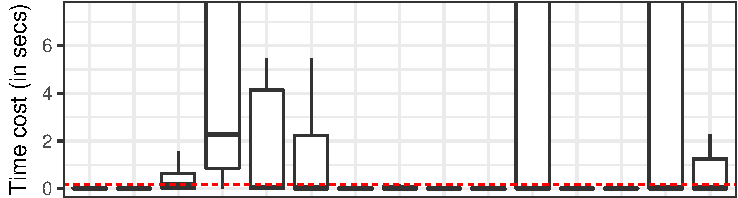
\includegraphics[width=\textwidth]{plots/testcost-long.pdf}
      \caption{\label{fig:longtcost}Long group.}
    \end{subfigure}\\
    \vspace{2ex}
    \begin{subfigure}{0.47\textwidth}
      \centering
      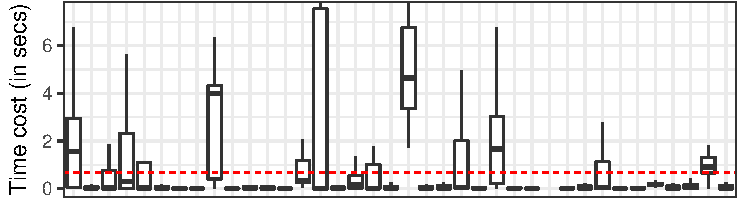
\includegraphics[width=\textwidth]{plots/testcost-medium.pdf}
      \caption{\label{fig:medtcost}Medium group.}
    \end{subfigure}
    %% \vspace{2ex}
    %% \begin{subfigure}{0.5\textwidth}
    %%   \centering
    %%   \begin{tabular}{rrrr}
    %%     \toprule
    %%     & $\sigma\leq1$ & $1<\sigma\leq5$ & $\sigma\ge5$ \\
    %%     \midrule    
    %%     Long   &  7 & 15 & 12 \\
    %%     Medium & 22 & 19 & 7 \\
    %%     \bottomrule
    %%   \end{tabular}
    %%   \caption{\label{fig:sd}Standard deviation ($\sigma$) of test case running times.}
    %% \end{subfigure}
    \caption{\label{fig:time-distributions}Time distributions.}%
\end{figure}

\sloppy Figures~\ref{fig:longtcost} and~\ref{fig:medtcost} show the
time distribution of individual test cases per project.  We observed
that the average median value of execution cost for a test was
relatively small (dashed horizontal red lines), namely 0.31s for
\medg{} projects and 0.23s for \longg{} projects.  The standard
deviations associated with each distribution were relatively
low.\Comment{ Figure~\ref{fig:sd} shows the number of projects within
  specific ranges of $\sigma$ values.}  We noted a small number of
cases of CPU monopolization.  For example, the highest value of
$\sigma$ occurred in \CodeIn{uber\_chaperone}, a project from the
medium group.  This project contains only 65 tests, 62 of which take
less than 0.5s to run, one of which takes nearly 3s to run, and two of
which take $\sim$40m to run.  For this project, 99.2\% of the
execution cost is dominated by only 3\% of the tests; without these
two costly tests this project would have been classified as
short-running.  A closer inspection in the data indicates that the
project \CodeIn{uber\_chaperone} was a corner case; we did not find
other projects with such extreme time monopolization profile.  Project
\CodeIn{facebookarchive\_linkbench} is also classified as long-running
and has the second highest value of $\sigma$.  For this project,
however, cost is distributed more smoothly across \Fix{529} tests, of
which \Fix{119 (23\%)} take more than \Fix{1s} to run with the rest of
the tests running faster.

\begin{figure}[t]
  \centering
  \begin{subfigure}{0.15\textwidth}
    \centering
    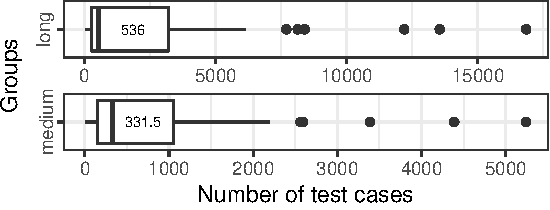
\includegraphics[width=.85\textwidth]{plots/boxplots-testcases.pdf}
    \caption{\label{fig:size-testsuites}Size of test suites.}
  \end{subfigure}
  ~
  \begin{subfigure}{0.3\textwidth}
    \centering
    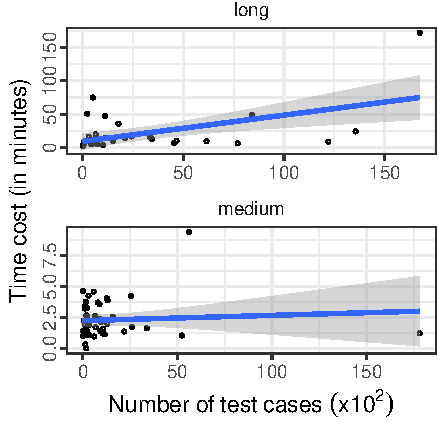
\includegraphics[width=.95\textwidth]{plots/scatter-testcost.pdf}
    \caption{\label{fig:scattercost}Size versus running time of
      test suites.}
  \end{subfigure}
  \caption{\label{fig:time-versus-size}Relating size and time.}%
\end{figure}

%\Mar{$\leftarrow$ show stats to indicate discrimination of
%  two distributions}

Figure~\ref{fig:time-distributions} showed that the average median
times were similar for \medg{} and \longg{}-running test suites.
Results indicate that the difference in overall running times of
projects in those groups was mainly justified by the number of test
cases as opposed to the individual costs of test cases.
Figure~\ref{fig:size-testsuites} shows the difference in the
distribution of test suite sizes across groups.  This figure indicates
that long projects, albeit having a wider inter-quartile range (middle
50\% projects in this group are less predictable), have a higher
median and much higher average number of test cases.  Furthermore, we
noted a strong positive correlation between running time and number of
test on projects in the \longg{} group.  Considering the \medg{}
group, the correlation between these two variables was weak.
Figure~\ref{fig:scattercost} illustrates this correlation.

%% however, weak in
%% the suggesting that saving time in this group with test suite
%% parallelization may be more challenging as relatively fewer tests
%% dominate overall execution time.  Figure~\ref{fig:scattercost} shows
%% these results.

%% This 
%% indication that it is more beneficial to parallelize long projects as
%% cost is spread across many

\vspace{1ex}
\begin{center}
\fbox{
\begin{minipage}{8cm}
    \textit{Answering \numRQFeasibilityTwo{}:}~\emph{Overall, results indicate that
    projects with a very small number of tests monopolizing end-to-end
    execution time were rare.}
\end{minipage}
}
\end{center}
\vspace{1ex}

%% We are interested to know whether
%% most of the execution cost of a subject is dominated by a small subset
%% of test cases or if the cost is nearly equally distributed. 

%% We also evaluated the dispersion of time distributions (one
%% distribution per project) to answer research question \numRQFeasibilityTwo{}.  To
%% measure dispersion \emph{across} projects we used Relative Standard
%% Deviation (RSD)~\cite{everitt-book-stats-2010}.  Note that, if we were
%% to analyze each project in isolation, the standard deviation of a
%% distribution ($\sigma$) would suffice to quantify how dispersed the
%% (time) distribution is.  However, in our case, we would like to be
%% able to compare and summarize dispersion across projects.  The RSD,
%% which is obtained dividing the standard deviation by the mean ($\mu$)
%% of a distribution, provides such normalization effect.  This metric
%% provides a lower bound (zero) but not an upper bound (somewhere close
%% to 1).  The smaller (larger) the value of RSD the more (less) uniform
%% the distribution is.  Consequently, the lower the value of RSD the
%% more parallelizable a test suite should be.

%% \begin{figure}[h!]
%%   \centering
%%   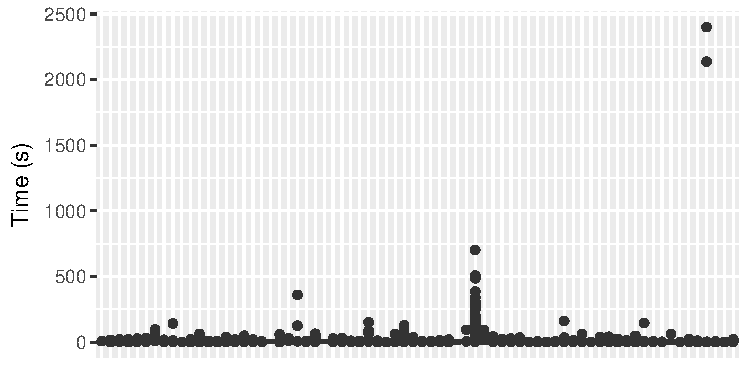
\includegraphics[width=0.5\textwidth]{R/testcost.pdf}  
%%   \caption{\label{fig:relativesd}Distribution of RSD ($\sigma/\mu$)
%%     across projects.}
%% \end{figure}

%% Figure~\ref{fig:relativesd} shows the distribution of RSD across
%% medium and long-running projects.  Results show that the distribution
%% is skewed to the right indicating that test costs are relatively well
%% distributed in most costly projects we analyzed \Fix{$\leftarrow$
%%   confirm}.

%% analyzed the execution time
%% for the \numMedLong{} projects from the \longg{} and \medg{} groups
%% (see Section~\ref{sec:rqA}).
%% For each subject we calculated the
%% relative standard deviation of the test cases: we collected the
%% elapsed time of each individual test, calculated the standard
%% deviation, and divided by the mean. \Jbc{I need to clarify the
%%   relationship "well/bad-balanced" regression test and relative
%%   standard deviation}

%% Results indicated that \Fix{...elaborate...}. \Jbc{We may identify
%% different groups of subjects}\Fix{TODO: collect data + compute the
%% statistic, create a scatter plot to identify groups of subjects}

%% Regression tests that are well distributed may benefit from
%% parallelism since more tests executes at the same time while the
%% opposite scenario may require a different approach. In the later
%% scenario, executing tests in parallel may have insignificant impact
%% since a small subset of test cases dominates the execution.}


\subsection{Adoption}
\label{sec:rqC}
\label{sec:rqE}

The dimension adoption focuses on the usage of parallelism in
open-source projects.  It evaluates (\numRQAdoptionOne) how often open-source
projects use parallelization schemes and (\numRQAdoptionTwo) how developers
involved in costly projects, not using parallelization, perceive this
technology.

\begin{itemize}
    \item \numRQAdoptionOne. \textbf{\RQAdoptionOne{}}
\end{itemize}

To answer \numRQAdoptionOne{}, we selected all projects from the \medg{} and
\longg{} groups, \ie, projects that ran in at least one minute.  This
set includes \numMedLong{} projects (see Section~\ref{sec:rqA}).  We
looked for dynamic and static manifestations of parallelism.

%% The
%% following section report results for each of these cases.

\vspace{1ex}
\subsubsection{Dynamic checking}
\label{sec:rqC-1}

To find dynamic evidence of parallelism, we ran the test suites from
our set of \numMedLong{} projects to output all key-value pairs of
Maven parameters.  To that end, we used the option~\CodeIn{-X} to
produce debug output and the option~\CodeIn{-DskipTests} to skip
execution of tests.  We skipped execution of tests as we observed from
sampling that only bootstrapping the Maven process suffices to infer
which parallel configuration modes it will use to actually run the
tests.  It is also important to point that we used the default
configurations specified in the project.  We inferred parallel
configurations by searching for certain configuration parameters in
log files. According to Maven's
documentation~\cite{maven-surefire-plugin}, a parallel configuration
depends either on (1) the parameter \CodeIn{parallel} to define the
parallelism mode within a JVM followed by the parameter
\CodeIn{threadCount} or (2) the parameter
\CodeIn{forkCount}\footnote{This parameter is named \CodeIn{forkMode}
  in old versions of Maven Surefire} to define the number of forked
JVMs.  As such, we captured, for each project, all related key-value
pairs of Maven parameters and mapped those pairs to one of the
possible parallelization modes.  For instance, if a given project
contains a module with the parameter
\CodeIn{<forkCount>1C</forkCount>}, the possible classifications are
\ForkSeq{} or \ForkParMeth{}, depending on the presence and the value
of the parameter \CodeIn{parallel}.  If the parameter
\CodeIn{parallel} is set to \CodeIn{methods} the detected mode will be
\ForkParMeth{}.  Large projects may contain several test suites
distributed on different Maven modules potentially using different
configurations.  For those cases, we collected the Maven output from
each module discarding duplicates as to avoid inflating counts for
configuration modes that appear in several modules of the same
project. For instance, if a project contains two modules using the
same configuration, we counted only one occurrence.


\begin{wrapfigure}{r}[0pt]{0pt}%0.525\linewidth
  \footnotesize
  %  \small
  \centering
  \setlength{\tabcolsep}{2.5pt}
%    \resizebox{.48\textwidth}{!}{%
    \begin{tabular}{lrr}
        \toprule
        \emph{Subject} & \emph{\# of modules} & \emph{Mode}\\%
        \midrule%
        \Comment{BounceStorage }Chaos\Comment{ HTTP Proxy} & 1/1 &  \ParClassSeqMeth{}\\%
        \Comment{Apache }Flink & 74/74 & \ForkSeq{} \\%        
        \Comment{JenkinsCI }Gerrit\Comment{ Trigger Plugin} & 1/1 & \ForkSeq{}\\%
        \Comment{Spotify }Helios & 8/8 & \ForkSeq{}\\%
        Javaslang & 3/3 & \ParClassParMeth{}\\%
        Jcabi\Comment{ Github} & 1/1 & \ParClassParMeth{}\\%        
        \Comment{Hazelcast }Jet & 7/14 & \ForkSeq{}\\%
        \Comment{Apache Logging }Log4J2 & 25/31 & \ForkSeq{}\\%
        \Comment{Jankotek }MapDB & 1/2 & \ParClassParMeth{}\\%        
        \bottomrule%
    \end{tabular}
    \caption{Subjects with parallel test execution enabled by
    default.}
    \label{tab:freqmodes-dynamic}
\end{wrapfigure}
Figure~\ref{tab:freqmodes-dynamic} shows the projects we idendified
where parallelism is enabled by default in Maven.  Column
``\emph{Subject}'' indicates the name of the project, column
``\emph{\# of modules}'' indicates the fraction of modules containing
tests that use the configuration of parallelism mentioned in column
``\emph{Mode}''.  We note that, considering these projects, the
modules that do not use the configuration cited use the sequential
configuration \Seq{}.  For example, six modules (=31-25) from Log4J2
use sequential configuration.

It came as a surprise the observation that
no project used distinct configurations in their modules. Considering
our set of \numMedLong{} projects, we found that only
\textbf{\numProjectsPar{}} of those projects had parallelism enabled
by default, with only configurations \ParClassSeqMeth{},
\ParClassParMeth{}, and \ForkSeq{} being used.  Configurations
\ParClassParMeth{} and \ForkSeq{} were the most popular among these
cases.  Note that these results under-approximate real usage of
parallelism as we used default parameters in our scripts to spawn the
Maven process.  That decision could prevent execution of particular
test modules.
%\begin{figure}[h!]
%    \centering
%    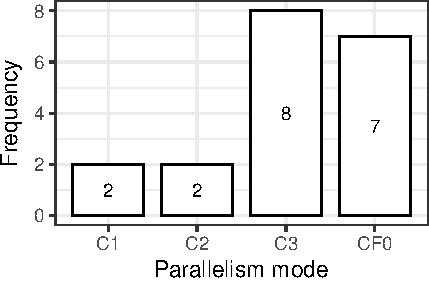
\includegraphics[width=0.32\textwidth]{plots/barplot-modes-dynamic.pdf}
%    \caption{\label{fig:freqmodes-dynamic}\Fix{fix
%    caption}Distribution of parallel modes identified dynamically in a
%    subset of \numProjectsPar{} projects.  A project may have support
%    to more than one parallel mode. Also, a project may run only a
%    subset tests in parallel by default.}
%\end{figure}

%% Recall that some projects can use parallel execution that is only
%% activated when developers pass certain parameters to the build
%% process. For instance, it is possible to create in Maven multiple
%% configurations in the same build file and select dynamically which one
%% should be used.  

\subsubsection{Static checking}
\label{sec:rqC-2}
Given the inherent limitation of dynamic monitoring to find evidence
of parallelism, we also looked for indication of parallelism in build
files\Comment{ in the same sample set of \numMedLong{} projects}.  We
parsed all \emph{pom.xml} files under the project's directory and used
the same approach as in our previous analysis to classify
configurations.  We noticed initially that our approach was unable to
infer the configuration mode for cases where the decision depends on
the input (\eg,
\CodeIn{<parallel>\$\{parallel.type\}</parallel>}). For these
projects, the tester needs to provide additional parameters in the
command line to enable parallelization (\eg, \CodeIn{mvn test
  -Dparallel.type=classesAndMethods}). To handle those case, we
considered all possible values for the parameter (in this case,
\CodeIn{\$\{parallel.type\}}).  It is also important to note that this
approach is not immune to false negatives, which can ocurr when
\emph{pom.xml} files are encapsulated in jar files or downloaded from
the network.  Consequently, this static checking is complementary to
the dynamic checking, previously presented.

Overall, we found, using this methodology, ten projects that use
parallelism.  Compared to the set of projects listed in
Figure~\ref{tab:speedup}, we found two new projects, namely:
\CodeIn{Google Cloud\Comment{ Platform} DataflowJavaSDK} (using
configuration C3) and \CodeIn{Mapstruct} (using configuration
\ForkSeq{}).  Curiously, we also found that project \CodeIn{Jcabi} was
not detected using this methodology.  That happened because this
project loads its \emph{pom.xml} file from a jar file that we did not
check.  Considering the static and dynamic methods together, we found
a total of 11 distinct projects using parallelism, corresponding to
the union of the two subject sets.

\vspace{1ex}
\begin{center}
\fbox{
  \begin{minipage}{8cm}
      \textit{Answering \numRQAdoptionOne{}:}~\emph{Results indicate that test
        suite parallelization is underused.  Overall, only
        \percentParallel{} of costly projects (11 out of \numMedLong)
        use parallelism.}
  \end{minipage}
}
\end{center}
\vspace{1ex}

%False positive can happen because of comments, for instance.  
%To eliminate the cases of false positives and also to categorize 
%true positive cases, we complemented the initial mining step with a 
%manual inspection of files.
%% settings); the second step (inspection) consists in a manual
%% inspection to confirm the presence of parallelism settings in the
%% build file and classify them according to the parallelism level.
%% Figure \Fix{removed} describes the discovery step: we list the paths
%% of all build files and filter only the files that contain any of the

%% Figure~\ref{tab:inspection-table} summarizes our results.
%% \Fix{The first column indicates the group of projects according to
%% their time cost.  The second column indicates the number of build
%% files per group.  The last column indicates the ratio of projects with
%% parallelization settings.  From the \numMedLong{} subjects, we found
%% \pomMedLong{} \pomf{} files.  The \numPomMatched{} configurations are
%% distributed across \numProjectsPar{} projects from our sample.}

%% % \emph{From these results we found that $\sim$51\% of medium and
%% % long-running projects do not use parallel features to run test
%% % suites.}\Mar{please make it consistent with research
%% % question}\Mar{explain this is over(under)-estimated...}
%% \begin{figure}[ht!]
%%     \centering
%%     \resizebox{.48\textwidth}{!}{%
%%     \begin{tabular}{llcl}
%%         \toprule
%%         Group & Subject & \# of modules & Mode\\%
%%         \midrule%
%%         Long   &JenkinsCI Gerrit Trigger Plugin& 1 & \ForkSeq\\%
%%         Medium &Bouncestorage Chaos Http Proxy & 1 & C2\\%
%%         Medium &Javaslang & 1 & C3\\%
%%         Medium &Apache Flink & 1 &\ForkSeq\\%
%%         Medium &Apache Logging Log4J2 & 3 & \ForkSeq{}\\%
%%         Medium &Google Cloud Platform DataflowJavaSDK & 1 & C3\\%
%%         Medium &Hazelcast Jet & 1 & \ForkSeq\\%
%%         Medium &Jankotek MapDB & 1 & C3\\%
%%         Medium &Mapstruct & 1 & \ForkSeq\\%
%%         Medium &Spotify Helios & 3 & \ForkSeq\\%
%%         \bottomrule%
%%     \end{tabular}}
%%     \caption{Subjects with parallelization configurations in build files.}
%%     \label{tab:inspection-table}
%% \end{figure}

%% \begin{figure}[ht!]
%%     \centering
%%     \begin{tabular*}{0.48\textwidth}{@{\extracolsep{\fill}}ccc}
%%         \toprule
%%         \multirow{2}{*}{Group} %1st row, 1st cell
%%             & \multirow{2}{*}{\# \pomf{}}
%% 	    & \# \pomf{} matched\\
%%         % 2nd row - empty cell
%%             & % empty cell
%%             & / total\\%
%%         \midrule%
%% 	Long   & \numPomLong{} & 4 / \numLong{}\\%
%% 	Medium & \numPomMed{} & 6 / \numMed{}\\%
%%         \midrule%
%%         Total % last row, first cell
%%             & \pomMedLong{}
%%             & \numProjectsPar{} / \numMedLong{}\\%
%%         \bottomrule%
%%     \end{tabular*}
%%     \caption{Presence of parallelization settings in build files: the
%%     first column indicates the group of projects according to their
%%     time cost; the second column is the subset of files with parallelization
%%     keywords; the last column indicates the ratio of projects with
%%     parallelism support.}
%%     \label{tab:inspection-table} 
%% \end{figure}
%% \Jbc{rework this... $\rightarrow$} From the \numProjectsPar{} projects
%% identified above, we investigated further the \numPomMatched{}
%% build files with parallel settings.  We analyzed the support and
%% distribution of parallel modes from this subset of projects. To
%% calculate the distribution of parallel modes, we considered only the
%% presence of the mode in at least one of the project settings.  Recall
%% that a build file may contain more than one parallel setting and a
%% project may contain several sub-modules with build files.  In case the
%% value of a parallel option is resolved dynamically (\eg, via
%% command-line argument or system variable) we compute all modes related
%% to the option. For instance, depending on the value, the
%% \CodeIn{parallel} option can be \Seq{} (\CodeIn{none}),
%% \ParClassSeqMeth{} (\CodeIn{classes}), \SeqClassParMeth{},
%% (\CodeIn{methods}), and \ParClassParMeth{} (\CodeIn{all}).
%% Figure~\Fix{fig:freqmodes-static} summarizes our findings.
%% \Fix{Missing conclusion: Fork the most used configuration}
%% \begin{figure}[h!]
%%     \centering
%%     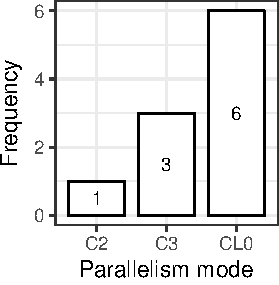
\includegraphics[width=0.32\textwidth]{plots/barplot-modes-static.pdf}
%% 	\caption{\label{fig:freqmodes-static}\Luis{This is wrong, it
%% 	should be \textbf{CF0} instead of \textbf{CL0}}Distribution of parallel modes
%%     identified statically in a subset of \numProjectsPar{} projects.
%%     A project may have support to more than one parallel mode.}
%% \end{figure}


\begin{itemize}
	\item \numRQAdoptionTwo{}. \textbf{\RQAdoptionTwo{}}
\end{itemize}

To answer this research question we surveyed developers involved in a
selection of projects from our benchmark with time-consuming test
suites.  The goal of the survey is to better comprehend developer's
attitude towards the use of parallelism as a mechanism to speedup
regression testing.  We surveyed developers from a total of
\emailsProjects{} projects.  From the initial list of \numMedLong{}
project, we discarded 11 projects that we knew a priori used
parallelization, and \discartedProjects{} projects that we could not find
developer's emails from commit logs.  From this list of projects, we
mined potential participants for our study.  More precisely, we
searched for developer's name and email from the last 20 commits to
the corresponding project repository.  Using this approach, we
identified a total of \emailsSent{} eligible participants.  Finally,
we sent plain-text e-mails, containing the survey, to those developers.  In
total, \emailsAnswered{} developers replied but we discarded
\emailsFalseAnswers{} replies with subjective answers.  Considering
projects covered by the answers, a total of \emailsProjectsAnswered{}
projects (\percEmailsProjectsAnswered{} of the total) were represented
in those replies.  Note that multiple developers on each project
received emails.  We sent the following set of questions to
developers:

\begin{enumerate}
\item How long does it take for tests to run in your environment? Can
  you briefly define your setup?
\item Do you confirm that your regression test suite does *not* run in parallel?
\item\label{questionThree} Select a reason for not using parallelization:
  \begin{enumerate}[label=\alph*)]
  \item I did not know it was possible
  \item I was concerned with concurrency issues
  \item I use a continuous integration server
  \item Some other reason. Please elaborate.
  \end{enumerate}
\end{enumerate}

%% \begin{enumerate}
%% 	\item How long does it take for test to run in your
%%		environment?
%%	\item Can you briefly define your setup?
%%	\item Do you confirm that your project does not run in
%%		parallel?
%%	\item Select a reason for not using paralellization:
%%		\begin{enumarate}
%%			\item I did not know it was possible;
%%			\item I was concerned with concurrency issues;
%%			\item I use a continuous integration server;
%%			\item Some other reason.
%%		\end{enumerate}
%% \end{enumerate}
%% One of the goals of the first questions is to identify potential
%% discrepancies between our experimental environment and the environment
%% of developers.  Overall, we found that \Fix{...}

Considering question 1, we confirmed that execution time was
compatible with the results we reported in Section~\ref{sec:rqA}.
Furthermore, \emailsCI{} of the participants indicated the use of
Continuous Integration (CI) to run tests, with \emailsDistributed{} of
these participants reporting that test suites are modularized and
those modules are tested independetly in CI servers through different
parameters.  Those participants argumented that such practice helps to
reduce time to observe test failures, which is the goal of speeding up
regression testing.  A total of \emailsLocal{} participants answered
that they do run tests in their local machines.  Note, however, that
CI does not preclude low-level parallelization.  For example,
installations of open-source CI tools (\eg{}, Jenkins~\cite{jenkins})
in dedicated servers would benefit from running tests faster through
low-level test suite parallelization.

% \emailsNotDescribed{} developers did not described their environment.

Considering question 2, the answers we collected indicated, to our
surprise, that six of the \emailsProjectsAnswered{} projects execute
tests in parallel.  This mismatch is justified by cases where neither
of our checks (static or dynamic) could detect presence of
parallelism.  A closer look at these projects revealed that one of
them contained a \emph{pom.xml} file encapsulated in a jar file
(similar case as reported in Section~\ref{sec:rqC-2}), in one of the
projects the particpant considered that distributed CI was a form of
parallelism, and in four projects the team preferred to implement
parallelization instead of using existing features from the testing
framework and the build system~---~in two projects the team
implemented concurrency control with custom JUnit test runners and in
two other projects the team implemented concurrency within test
methods.  Note that, considering these four extra cases (ignored two
distributed CI cases), the usage of parallelization increases from
\percentParallel{} to \percentParallelUpdated{}.  We do not consider
this change significant enough to modify our conclusion about
practical adoption of parallelization (\numRQAdoptionOne{}).

%% , one runs a manually created Thread to run some
%% tests, and the other runs in parallel by using Java 8 collection
%% streams, that allows the developers to iterate over a list in
%% parallel.

%% did not confirmed, however,
%% the developers confirmed the need of an extra parameter at the command
%% line to execute in parallel.

Considering question 3, the distribution of answers was as follows.  A
total of \emailsA{} of the \emailsProjectsAnswered{} developers who
answered the survey did not know that parallelism was available in
Maven (option ``a''), \emailsB{} of developers mentioned that they did
not use parallelism concerned with possible concurrency issues (option
``b''), \emailsD{} of developers mentioned that continuous integration
services sufficed to provide timely feedback while running only smoke
\begin{wrapfigure}{r}[0pt]{0pt}%0.525\linewidth
    \centering
    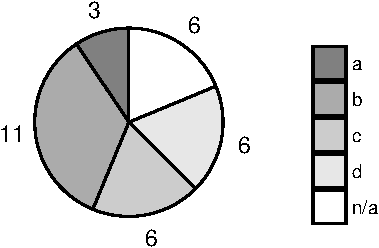
\includegraphics[width=.18\textwidth]{plots/survey.pdf}
    \caption{\label{fig:rq5-answers}Summary of developer's answers to
      survey question~\ref{questionThree}.}
\end{wrapfigure}
tests (\ie{}, short-running tests) locally (option ``c'')\Comment{here
  I want to say that they use it for something like "non-blocking
  testing" while developing in a local machine}, and \emailsD{} of
developers who provided an alternative answer (option ``d'') mentioned
that using parallelism was not worth the effort of preparing the test
suites to take advantage of available processing power.  A total of
\emailsNA{} of participants did not answer the last question of the
survey.  The pie chart in Figure~\ref{fig:rq5-answers} 
summarizes the distribution of answers.

\begin{center}
\fbox{
	\begin{minipage}{8cm}
	  \textit{Answering \numRQAdoptionTwo{}:}~\emph{Results suggest that dealing
       with concurrency issues (\ie{}, the extra work to organize test
       suite to safely explore concurrency) was the principal reason
       for developers not investing in parallelism.  Other reasons
       included availability of continuous integration services and
       unfamiliarity with the technology.}
	\end{minipage}
}
\end{center}

\subsection{Speedups}
\label{sec:rqD}

\begin{itemize}
    \item \numRQSpeedupOne{}. \textbf{\RQSpeedupOne}
\end{itemize}

To answer \numRQSpeedupOne{}, we considered the \numProjectsPar{}
subjects from our benchmark that use parallelization \emph{by default}
(see Figure~\ref{tab:freqmodes-dynamic}).  We compared running times
with parallelization~---~configured by project owners~---~and without
parallelization.

%% In those projects, parallelization is active without
%% passing any extra parameters.  Section~\ref{sec:rqC-1} describes in
%% detail the methodology we used to find these subjects.
%and
%Section~\ref{seq:rq6-tradeoffs}, we verified that both
%% executions produce the same outcome to eliminate noise from failing
%% tests.  To compute the speedup, we divide the time obtained in the
%% sequential execution by the time obtained from the default execution.
%% For instance, if a project runs the tests sequentially in $10m$ and
%% the same execution runs in $5m$ with parallelization enabled (default
%% execution), the speedup is two.

Figure~\ref{tab:speedup} summarizes results.  Lines are sorted by
project names.  Columns ``\emph{Group}'' and
``\emph{Name}'' indicate, respectively, the group and the name of the
subject.  Column ``$T_s$'' shows sequential execution time and column
``$T_p$'' shows parallel execution time. Column ``$T_s/T_p$'' shows
speedup or slowdown.  As usual, a ratio above 1x denotes speedup
and a ratio below 1x denotes slowdown.

\begin{figure}[h!]
\centering
\resizebox{.41\textwidth}{!}{%
  \scriptsize
\begin{tabular}{llrrr}
\toprule
\emph{Group} & \emph{Subject} & \multicolumn{1}{c}{$T_s$} & \multicolumn{1}{c}{$T_p$} & $T_s/T_p$ \\%
\midrule%
Medium & \Comment{BounceStorage }Chaos\Comment{ HTTP Proxy} & 1.51m & 1.47m & 
    \cellcolor{lightgray}1.01x\\%
Medium &\Comment{ Apache }Flink& 11.79m & 2.57m & 4.59x\\%
Long &\Comment{ Jenkins CI }Gerrit\Comment{ Plugin} & 51.19m & 40.31m &  1.26x\\%
Medium &\Comment{ Spotify }Helios& 4.46m & 1.63m & 2.73x\\%  
Medium &Javaslang& 2.18m & 1.82m & 1.19x\\%
Medium &Jcabi\Comment{ GitHub} & 2.76m & 0.30m &
    \cellcolor{lightgray}9.2x\\%
Medium &\Comment{ Hazelcast }Jet& 8.26m & 3.67m & 2.25x\\%
Long &\Comment{ Apache }Log4J2& 8.24m & 8.21m & \cellcolor{lightgray}1.00x\\%
Long &\Comment{ Jankotek }MapDB& 10.06m & 8.58m & 1.17x\\%
\midrule
\textbf{average} &  &  &  & \avgSpeedup{}x\\
\bottomrule%
\end{tabular}}
\caption{\label{tab:speedup}Speedup (or slowdown) of parallel
  execution ($T_p$) over sequential execution ($T_s$).  Default
  parallel configuration of Maven is used.  Highest slowdown/speedup
  appears in gray color.}
\end{figure}

Results indicate that, on average, parallel execution was
\avgSpeedup{} times faster compared to sequential execution.  Three
cases worth special attention: \CodeIn{Chaos}, \CodeIn{Jcabi} and
\CodeIn{Log4J2}.  No significant speedup was observed in
\CodeIn{Chaos}, a project with only three test classes, of which one
monopolizes the bulk of test execution time.  This project uses
configuration \ParClassSeqMeth{}, which runs test classes in parallel
and test methods, declared in each class, sequentially.  Consequently,
speedup cannot be obtained as the cost of the single expensive test
class cannot be broken down with the selected configuration.  Although
project \CodeIn{Jcabi} also uses configuration \ParClassSeqMeth{},
results obtained are very different compared to \CodeIn{Chaos}.  The
speedup observed in \CodeIn{Jcabi} was the highest amongst all
projects.  This project contains test classes with a small number of
test methods and several methods in those classes are time-consuming.
As result, the CPUs available for testing are kept occupied for the
most part during test execution.  Finally, we note that parallel
execution in \CodeIn{Log4J2} was innefective.  We found that Maven
invokes several test modules in this project but the test modules that
dominate execution time run sequentially by default.

%% The third, runs parallel configuration in
%% \Fix{80\%} of the project modules, however, the test time is dominated
%% by one of the sequentially running modules.  \Luis{$\leftarrow$ rework
%%   this} \Fix{falar sobre o resultado geral dos speedups - elaborar
%%   menor e maior speedup... acho que so vale a pena discutir quando
%%   tiver conviccao dos 2 casos}

\begin{center}
\fbox{
  \begin{minipage}{8cm}
    \textit{Answering \numRQSpeedupOne{}:}~\emph{Considering the
      machine setup we used, the average speedup observed with default
      configurations of parallelization was \avgSpeedup{}x.}
  \end{minipage}
}
\end{center}

\begin{itemize}
    \item \numRQSpeedupTwo{}. \textbf{\RQSpeedupTwo}
\end{itemize}

\newcommand{\subjectScalability}{MapDB}

This experiment evaluates the impact of making available to the build
system a growing number of CPUs for testing.  For that reason, we used
a machine with more cores compared to the one described in
Section~\ref{sec:setup}.  We used a Xeon E5-2660v2 (2.20GHz) Intel
processor machine with 80 virtual CPUs (40 cores with two native
threads each) and 256GB of memory, running Ubuntu 14.04 LTS Trusty
Tarr (64-bit version). This experiment uses configuration \ForkSeq{}
\begin{wrapfigure}{r}[0pt]{0pt}%0.525\linewidth
    \centering
    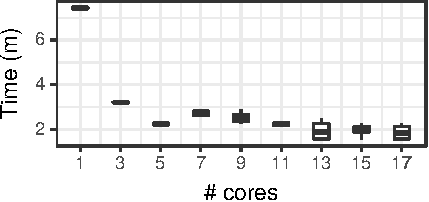
\includegraphics[width=.2\textwidth]{R/scalability/scalability.pdf}
    \caption{\label{fig:scalability}Scalability.}
\end{wrapfigure}
as the goal is to evaluate the impact on runtime of spawning a growing number of
JVMs in different CPUs.  Furthremore, we selected subject
\subjectScalability{} as it represents the case of a long-running test
suite (see Figure~\ref{tab:speedup}) with test cases distributed
across many test classes (194 test classes for \subjectScalability{}).
Note that a test class is the smallest unit that can be used to spawn
a test job on a JVM and that we have no control over which test
classes will be assigned to which JVM that the build system forks.

Figure~\ref{fig:scalability} shows the reduction of running times as
more CPUs contribute to the execution.  \Fix{elaborate...}

\begin{center}
\fbox{
  \begin{minipage}{8cm}
    \textit{Answering \numRQSpeedupTwo{}:}~\emph{...}
  \end{minipage}
}
\end{center}

\subsection{Issues}
\label{sec:rq6-tradeoffs}

This dimension assesses the impact of using distinct parallel
configurations on test flakiness (negative impact) and speedup
(positive impact).  Furthermore, note that Section~\ref{sec:rqD}
evaluated speedup in isolation, focused on projects configured to use
parallelism by default.

\begin{itemize}
    \item \numRQIssuesOne{}. \textbf{\RQIssuesOne{}}
\end{itemize}


%% The intuition is that efficiency and flakiness are inversely
%% proportional in some cases: if too many tests depends on the state of
%% a single external resource, several tests are likely to fail as the
%% degree of concurrency increases by exploiting maximum CPU usage.

%% Table header macros
% $\Uparrow_\text{speed}$
\newcommand{\subcolA}{$\text{speedup}$}
\newcommand{\subcolB}{$\%_\text{fail}$}
\newcommand{\colheader}[1]{\multicolumn{2}{c}{\emph{#1}}}
\newcommand{\blankentry}{\entry{-}{-}}
\newcommand{\subcol}{\subcolA{} & \subcolB{}}
\newcommand{\entry}[2]{#1 & #2}

\begin{figure*}[t]  
\centering
\small
\setlength{\tabcolsep}{3pt}
\begin{tabular}{l|rr|rr|rr|rr|rr|rr}
\toprule
\multirow{2}{*}{\emph{Subject (module)}} & \multicolumn{2}{c|}{\emph{\Seq}} &
    \colheader{\SeqClassParMeth} & \colheader{\ParClassSeqMeth} &
    \colheader{\ParClassParMeth} & \colheader{\ForkSeq} &
    \colheader{\ForkParMeth} \\ %\cline{2-12}
    & $T$ & $\mathit{N}$ & \subcol{} & \subcol{} & \subcol{} & \subcol{}
    & \subcol{}\\%
\midrule%
AWS SDK Java (\CodeIn{core})  & \entry{3.7m}{847}  & \entry{1.95x}{2.24\%} & \entry{2.47x}{2.77\%} & \entry{3.70x}{4.01\%} & \entry{}{} & \entry{}{}\\%

Facebook Linkbench    & \entry{4.3m}{98}  & \entry{1.00x}{0\%} & \entry{1.65x}{1.02\%} & \entry{1.59x}{1.02\%} & \entry{}{} & \entry{}{}\\%

GoogleCloud Dataflow Java (\CodeIn{sdk}) & \entry{1.6m}{3,345}  & \entry{1.23x}{1.67\%} & \entry{2.67x}{1.05\%} & \entry{0.80x}{5.35\%} & \entry{}{} & \entry{}{}\\%

Javaslang (\CodeIn{core})     & \entry{1.1m}{17,513}  & \entry{1.38x}{0\%} & \entry{1.83x}{0\%} & \entry{1.38x}{0\%} & \entry{}{} & \entry{}{}\\ 
JCabi Github                  & \entry{2.6m}{634} & \entry{2.10x}{0\%} & \entry{17.70x}{0\%} & \entry{28.80x}{0\%} & \entry{}{} & \entry{}{} \\
JCTools (\CodeIn{core})       & \entry{3.6m}{690}  & \entry{4.50x}{0\%} & \entry{3.60x}{0\%} & \entry{18.00x}{0\%} & \entry{}{} & \entry{}{}\\%
MapDB  & \entry{8.2m}{5,324}  & \entry{1.52x}{0\%} & \entry{2.73x}{0\%} & \entry{4.82x}{0.05\%}   & \entry{}{} & \entry{}{}\\%
Moquette                      & \entry{3.7m}{169} & \entry{4.62x}{65.64\%} & \entry{3.36x}{32.92\%} & \entry{12.33x}{77.78\%} & \entry{}{} & \entry{}{} \\
RipMe                         & \entry{1.1m}{54}  & \entry{0.94x}{0\%} & \entry{1.63x}{0\%} & \entry{1.63x}{0\%} & \entry{1.37x}{0\%} & \entry{1.42x}{0\%}\\
Stripe Java     & \entry{4.3m}{302}  & \entry{4.78x}{6.31\%} & \entry{3.31x}{7.31\%} & \entry{21.50x}{14.95\%} & \entry{}{} & \entry{}{}\\%





\midrule

\textbf{Average}   & \entry{-}{-} & \entry{-}{-} & \entry{-}{-} & \entry{-}{-}
& \entry{-}{-} & \entry{-}{-} \\%


%%  & \entry{x.xm}{0}  & \entry{}{\%} & \entry{}{\%} & \entry{}{\%} & \entry{}{} & \entry{}{}\\%
%%OpenMRS Core (\CodeIn{api})  & \entry{15.4m}{3436} & \blankentry{}        & \blankentry{}        & \blankentry{} & \entry{1.5x}{0\%} & \entry{1.7x}{0}\\%
%%Apache Flume (\CodeIn{core}) &  \entry{7.7m}{392}  & \blankentry{}        & \blankentry{}        & \blankentry{}       & \entry{0.9x}{0\%} & \blankentry{} \\%
%%Facebook Archive Linkbench   &  \entry{4.5m}{98}   & \entry{1.0x}{0.2\%}  & \entry{1.6x}{1.2\%}       & \entry{1.0x}{0\%}  & \entry{1.7x}{0.5\%}  & \entry{1.7x}{0.2\%}\\%
%%AWS SDK Java (\CodeIn{core}) &  \entry{3.8m}{847}  & \multicolumn{6}{c}{\Fix{requires investigation}} & \entry{2.2x}{0.1\%} & \entry{3.2x}{2.0\%}\\%

%% OpenMRS Core (\CodeIn{api})  & \entry{15.4m}{3436} & \blankentry{}        & \blankentry{}        & \blankentry{} & \entry{1.5x}{0\%} & \entry{1.7x}{0}\\%
%% Jankotek MapDB               &  \entry{9.9m}{5218} & \multicolumn{6}{c}{\cellcolor{lightgray}\emph{JVM Crash}} & \entry{1.5x}{0\%} & \entry{1.7x}{0\%}\\%
%% Apache Flume (\CodeIn{core}) &  \entry{7.7m}{392}  & \blankentry{}        & \blankentry{}        & \blankentry{}       & \entry{0.9x}{0\%} & \blankentry{} \\%
%% Apache Giraph (\CodeIn{core})&  \entry{7.2m}{236}  & \entry{2.1x}{5.1\%}  & \colheader{\cellcolor{lightgray}timeout}   & \entry{1.0x}{0\%} & \entry{1.0x}{0}\% & \colheader{\cellcolor{lightgray}JVM Crash}\\%
%% Facebook Archive Linkbench   &  \entry{4.5m}{98}   & \entry{1.0x}{0.2\%}  & \entry{1.6x}{1.2\%}       & \entry{1.0x}{0\%}  & \entry{1.7x}{0.5\%}  & \entry{1.7x}{0.2\%}\\%
%% Stripe Java                  &  \entry{4.2m}{302}  & \entry{4.2x}{5.2\%}  & \entry{3.5x}{5.7\%}       & \entry{4.2x}{6.3\%} & \entry{1.0x}{0.3\%} & \entry{4.2x}{5.7\%}\\%
%% AWS SDK Java (\CodeIn{core}) &  \entry{3.8m}{847}  & \multicolumn{6}{c}{\Fix{requires investigation}} & \entry{2.2x}{0.1\%} & \entry{3.2x}{2.0\%}\\%

%% Jenkins CI Github            & \entry{Xm}{Z}       & \entry{x}{\%}          & \entry{x}{\%} & \entry{x}{\%} & \entry{x}{\%} & \entry{x}{\%}\\%
%% Jenkins CI Docker Workflow   & \entry{Xm}{Z}       & \entry{x}{\%}          & \entry{x}{\%} & \entry{x}{\%} & \entry{x}{\%} & \entry{x}{\%}\\%
%% Hazelcast                    & \entry{Xm}{Z}       & \entry{x}{\%}          & \entry{x}{\%} & \entry{x}{\%} & \entry{x}{\%} & \entry{x}{\%}\\%

\bottomrule%
\end{tabular}
\caption{Speedup versus Flakiness (\subcolB). Configuration
  \emph{\Seq{}} denotes the comparison baseline, which runs tests
  sequentially.  Columns $T$ and $N$ indicate time and number of
  tests, respectively.  Other columns show speedup and percentage of
  failing tests in different configurations, compared to
  \emph{\Seq{}}.\Mar{Can you please add name of module for all subjects?}}
\label{tab:rq6-table}
\end{figure*}

To answer this research question, we conducted an experiment involving
the six parallel configurations from Section~\ref{sec:modes}  and the
top 10 long-running test modules from our sample set. The rationale
for this selection criteria was to maximize the chances of observing
speedup and flakiness, assuming that long-running tests also have many
tests. Indeed, we confirmed that test suites in these projects contain
at least 236 tests ($1,662.7$ in average). Also, we preferred to compare the
effect of a configuration over a single test module for projects with
multiple test modules.  Recall that large projects may contain several
test modules, and these modules may contain distinct characteristics
that could favor one configuration and not others; therefore, it would
be necessary to check each module individually for a fair comparison.
We are interested in understanding how efficiency (\ie, testing cost)
and flakiness (\ie, failing tests) are affected when we run a test
suite with different parallel configurations.  Recall that increased
resource contention obtained with parallelism can lead to concurrency
issues such as data races.  Flakiness and speedup are contradictory
forces that drive configuration selection.  We used as a \emph{control
group} (\ie, baseline) the sequential execution of each subject's
tests. Notice that for measuring flakiness, we have to consider only
tests that failed due to the concurrency in the parallel execution.
For that reason, we re-executed the tests in sequence ten times and
carefully verified that there are only passing tests in our baseline.
We considered ten as the number of re-executions based on the approach
used by Google reported in a previous work on test
flakiness~\cite{luo-etal-fse2014}.  To obtain parallel configurations,
we implemented a script that takes a subject and a configuration (\eg,
\ForkSeq{}) as inputs, and the script outputs the modified version of
the subject with the desired configuration. The workflow consists in
copying the project directory to a new directory, finding all existing
build files (\ie, \pomf{} files), and modifying all existing Maven
Surefire configurations with new values for the parameters
\CodeIn{parallel}, \CodeIn{forkCount}, and \CodeIn{threadCount} using
an XPath~\cite{xpath} library to manipulate XML documents. For
configurations with forked JVMs enabled (\ie, \ForkSeq{} and
\ForkParMeth{}), we changed the \CodeIn{forkCount} with the value
\CodeIn{1C} (\ie, one JVM per core).  To adjust the pool of threads
for parallelism within a JVM, we changed the parameter
\CodeIn{threadCount} with \Jbc{should we consider 2 as it is the
number of native threads per core OR 6 as it represents 3 Cores * 2
native threads?}.  To run the subjects and their respective variations
(\ie, the modified versions according to the parallelism
configuration), we used a similar approach as described in


Figure~\ref{fig:mvn-execution} except that we added a timeout of one
hour to run the tests. We used the \CodeIn{timeout}
command~\cite{timeout-cmd} to monitor the execution, and we configured
the command to dispatch a \emph{kill} signal if the test execution
exceeds the time limit. We imposed this time constraint to avoid
hanging indefinitely the experiment execution due to some thread
contention that may occur (\eg, deadlock). Finally, we saved each
execution log and XML test reports generated by Maven to collect the
execution time, the number of failing tests, and for reference to
analyze and diagnose outliers in our results. For efficiency, we
reported the speedup (\ie, $\Uparrow_\text{speed} = T_{\text{s}} /
T_{\text{p}}$) in average, and for flakiness, we reported the rate of
failing tests (\ie, $\mathit{\%_\text{fail} = failures / tests}$) in
average.  Figure~\ref{tab:rq6-table} summarizes the obtained results
ordered by the time cost (\ie, $T_\text{cost}$). \Fix{Remember to
explain efficiency cutoff, JVM crashes and timeout}

\Jbc{Lembrar que investigar o slowdown de Dataflow... os logs indicam que varios
dos testes que quebraram tentavam fazer uma autenticacao em algum servico.
Possivelmente o slowdown se deve ao tempo de resposta do servico quando
a autentiticao falha}

%% \begin{figure}[h!]
%% \centering
%% \resizebox{.48\textwidth}{!}{%
%% \begin{tabular}{lcrrrrr}
%% \toprule
%% \emph{Subject} & \emph{\# of tests} & \emph{\SeqClassParMeth{}} & \emph{\ParClassSeqMeth{}} & \emph{\ParClassParMeth{}} & \emph{\ForkSeq{}} & \emph{\ForkParMeth{}}\\%
%% \midrule%
%% Linkedin Pinot & 356 & - & - & - & - & -\\%
%% %% Jenkins CI Github Plugin & - & - & - & - & 0\% & -\\%
%% %% Kite SDK & - & - & - & - & - & -\\%
%% %% \Fix{!?} Apache Giraph & 327 & - & - & - & - & -\\%
%% %% OpenMRS Core & - & - & - & - & - & -\\%
%% %% Jenkins CI Docker Workflow Plugin & - & - & - & - & 0\% & -\\%
%% %% \Fix{Flaky} Apache Eagle & - & - & - & - & - & -\\%
%% %%Geotools & 7701 & - & - & - & - & -\\%
%% %%Kuromoji & 672 & - & - & - & - & -\\%
%% %%Atomix & 99 & - & - & - & - & -\\%
%% %%\Fix{Snazy OHC} & - & - & - & - & - & -\\%
%% %%\Fix{RoaringBitmap} & - & - & - & - & - & -\\%
%% \bottomrule%
%% \end{tabular}}
%% \caption{\Fix{Tabela de flakiness}}
%% \label{tab:rq6-flaky}
%% \end{figure}

\Fix{Elaborate results from efficiency}

\Fix{Elaborate results from flakiness}

\Fix{highlight special cases}

\Fix{Draw conclusions}

\begin{center}
\fbox{
\begin{minipage}{8cm}
\textit{Answering \numRQIssuesOne{}:~\emph{\Jbc{summarize findings...}}}
\end{minipage}
}
\end{center}

%%  LocalWords:  RQ occurence parallelization Tradeoffs API readme th
%%  LocalWords:  mvn clearcut escapeinside xleftmargin untestable LTS
%%  LocalWords:  framexleftmargin CPUs Tahr sysstat gh Vagrantfile
%%  LocalWords:  javadoc isolcpus JUnit's JUnitCore Gligoric boxplots
%%  LocalWords:  outliers apache uber chaperone facebookarchive
%%  LocalWords:  linkbench priori


We ran the test suite for each subject three times, reporting averaged
execution times in three ranges: tests that run within a minute
(\shortg{} group), tests that run in one to five minutes (\medg{}
group), and tests that run in five or more minutes (\longg{}
group). We followed a similar methodology to group projects by time as
Gligoric~\etal{}~\cite{gligoric-etal-issta2015} in their work on
regression test selection.\Comment{ and added the \medg{} group due to
  the variability of the time cost from subjects out of the \shortg{}
  group} Figure~\ref{fig:rq1-barplot} shows the number of projects in
each group.  As expected, \longg{} and \medg{} projects do not occur
as frequently as \shortg{} projects.  However, they do occur in
relatively high numbers.

Figure~\ref{fig:rq1-boxplot} shows cost distribution of test suites in
each group as boxplots.  Note that the y-ranges are different.  The
distribution associated with the \shortg{} group is the most
unbalanced (right skewed)\Comment{ with outliers closed to the \medg{}
  group}.  The test suites in this group ran in 15 or less seconds for
over 75\% of the cases.  Such scenarios constitute the majority of the
cases we analyzed.  Considering the groups \medg{} and \longg{},
however, we found many costly executions.  Nearly 75\% of the projects
from the \medg{} group take over 3.5 minutes to run and nearly 75\% of
the projects from the \longg{} group take $\sim$20 minutes to run.  We
found cases in the \longg{} group were execution takes over 50 minutes
to complete, as can be observed from the outliers (dots) in the plot.

%% the median from the
%% \medg{} group is nearly two minutes and most of the subjects run in
%% less than four minutes; most of the \longg{} group runs in less than
%% 25 minutes but has outliers that require more than 50 minutes to
%% execute.



\begin{figure}[ht]
    \centering
    \begin{subfigure}{0.182\textwidth}
        \centering
        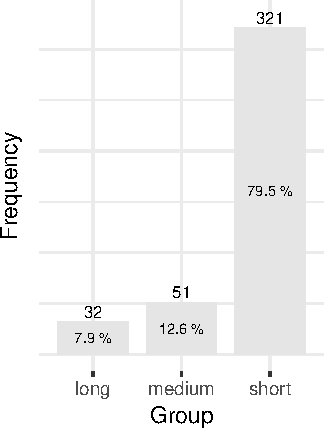
\includegraphics[width=\textwidth]{plots/barplot-timecost.pdf}
        \caption{\label{fig:rq1-barplot}}
    \end{subfigure}%
    ~
    \begin{subfigure}{0.25\textwidth}
        \centering
        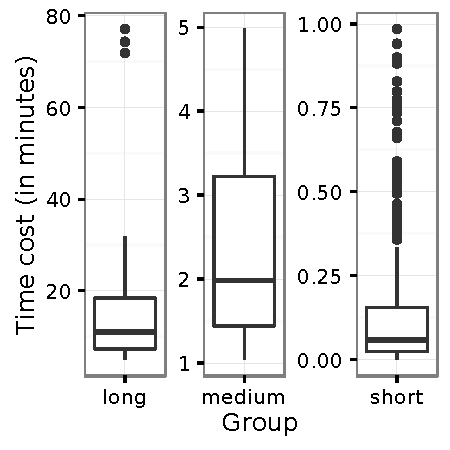
\includegraphics[width=\textwidth]{plots/boxplot-timecost.pdf}
        \caption{\label{fig:rq1-boxplot}}
    \end{subfigure}%
    \caption{(a) Subjects grouped by time cost ($t$): short run ($t <
    1m$), medium run ($1m \le t < 5m$), and long run ($5m \le t$); (b)
    Distribution of time cost by group.}
\end{figure}

%% Figure~\ref{fig:rq1-barplot} is a lower bound estimation of cost
%% because some tests may finish earlier than expected due to existing
%% test failures in the revision we downloaded.

It is important to note that we under-estimated cost in our
experiments for two main reasons.  First, some tests may finish
earlier than expected due to the observed test failures in some of the
revisions we downloaded.  From the \numSubjs{} testable projects,
\numSubjsPass{} successfully executed all tests and \numSubjsFail{}
reported some test failures.  Second, some projects may omit
long-running tests on their default execution. For instance, the
project \CodeIn{apache.maven-surefire} runs all unit tests in a few
seconds.  According to our criteria, this project is to be classified
as \shortg{} but a closer look reveals that only smoke tests are run
by default in this project.  Time-consuming integration and system
tests are only accessible via custom parameters, which we do not
handle in our experimental setup.  We enabled such parameters for this
specific project and observed that testing time goes to nearly 30
minutes.  For simplicity, we considered only the tests executed by
default.

\vspace{1ex}
\begin{center}
\fbox{
\begin{minipage}{8cm}
    \textit{Answering \numRQFeasibilityOne{}:}~\emph{We conclude that
      time-consuming test suites are relatively frequent in
      open-source projects.  We found that \percentMedLongRunning{} of
      the \numSubjs{} projects we analyzed (\ie{}, over 1 in every 5
      projects) take at least 3 minutes to run and
      \percentLongRunning{} take at least 5 minutes to run.\Comment{
        (\ie, \numMedLong{} projects from \medg{} and \longg{}).}}
\end{minipage}
}
\end{center}
\vspace{1ex}


\begin{itemize}
    \item \numRQFeasibilityTwo. \textbf{\RQFeasibilityTwo}
\end{itemize}

Section~\ref{sec:rqA} showed that medium and long-running projects are
not uncommon, accounting to nearly \percentMedLongRunning{} of the
\numSubjs{} projects we analyzed.  Research question \numRQFeasibilityTwo{}
measures the distribution of test costs in test suites as to estimate
(lack of) potential of obtaining speedups with parallelization.  In
the limit, if cost is dominated by a single test from a large test
suite, it is unlikely that parallelization will be beneficial as a
test method is the smallest working unit in test frameworks.

%% However, avoiding
%% frequent context switches is another factor to consider.  For example,
%% assuming there are at least two CPUs available for execution, cost can
%% be cut in half if two tests in a large test suite dominate execution
%% time and these tests are assigned to different CPUs.

%% It is therefore important to
%% speedup regressing testing in open-source projects.\Comment{not only
%%   to huge projects as those from Google~\cite{google-tap,google-ci}
%%   and Microsoft~\cite{prasad-shulte-ieee-microsoft-ci}.}



%% For the case
%% where cost is distributed more evenly across test cases, one expects
%% that speedups will be a function of the number of cores.
%% These contradictory forces, pushing number of tests and cost
%% of each test up and down, make prediction of effectiveness challenging.

\begin{figure}[h]
    \centering
    \begin{subfigure}{0.47\textwidth}
      \centering
      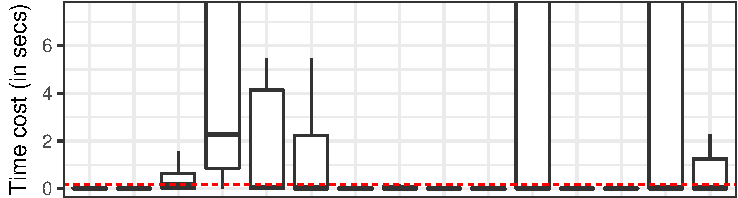
\includegraphics[width=\textwidth]{plots/testcost-long.pdf}
      \caption{\label{fig:longtcost}Long group.}
    \end{subfigure}\\
    \vspace{2ex}
    \begin{subfigure}{0.47\textwidth}
      \centering
      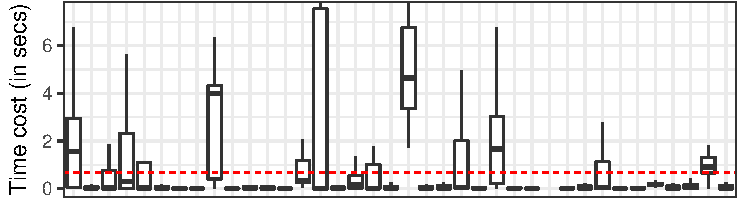
\includegraphics[width=\textwidth]{plots/testcost-medium.pdf}
      \caption{\label{fig:medtcost}Medium group.}
    \end{subfigure}
    %% \vspace{2ex}
    %% \begin{subfigure}{0.5\textwidth}
    %%   \centering
    %%   \begin{tabular}{rrrr}
    %%     \toprule
    %%     & $\sigma\leq1$ & $1<\sigma\leq5$ & $\sigma\ge5$ \\
    %%     \midrule    
    %%     Long   &  7 & 15 & 12 \\
    %%     Medium & 22 & 19 & 7 \\
    %%     \bottomrule
    %%   \end{tabular}
    %%   \caption{\label{fig:sd}Standard deviation ($\sigma$) of test case running times.}
    %% \end{subfigure}
    \caption{\label{fig:time-distributions}Time distributions.}%
\end{figure}

\sloppy Figures~\ref{fig:longtcost} and~\ref{fig:medtcost} show the
time distribution of individual test cases per project.  We observed
that the average median value of execution cost for a test was
relatively small (dashed horizontal red lines), namely 0.31s for
\medg{} projects and 0.23s for \longg{} projects.  The standard
deviations associated with each distribution were relatively
low.\Comment{ Figure~\ref{fig:sd} shows the number of projects within
  specific ranges of $\sigma$ values.}  We noted a small number of
cases of CPU monopolization.  For example, the highest value of
$\sigma$ occurred in \CodeIn{uber\_chaperone}, a project from the
medium group.  This project contains only 65 tests, 62 of which take
less than 0.5s to run, one of which takes nearly 3s to run, and two of
which take $\sim$40m to run.  For this project, 99.2\% of the
execution cost is dominated by only 3\% of the tests; without these
two costly tests this project would have been classified as
short-running.  A closer inspection in the data indicates that the
project \CodeIn{uber\_chaperone} was a corner case; we did not find
other projects with such extreme time monopolization profile.  Project
\CodeIn{facebookarchive\_linkbench} is also classified as long-running
and has the second highest value of $\sigma$.  For this project,
however, cost is distributed more smoothly across \Fix{529} tests, of
which \Fix{119 (23\%)} take more than \Fix{1s} to run with the rest of
the tests running faster.

\begin{figure}[t]
  \centering
  \begin{subfigure}{0.15\textwidth}
    \centering
    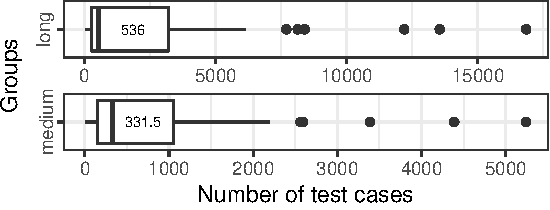
\includegraphics[width=.85\textwidth]{plots/boxplots-testcases.pdf}
    \caption{\label{fig:size-testsuites}Size of test suites.}
  \end{subfigure}
  ~
  \begin{subfigure}{0.3\textwidth}
    \centering
    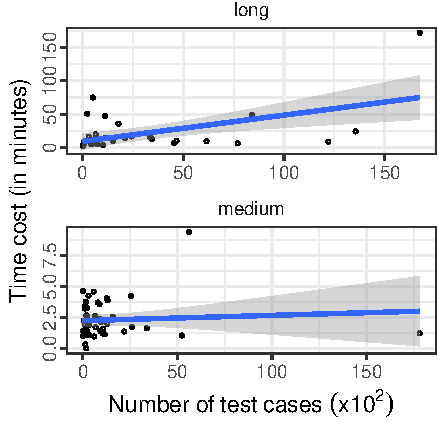
\includegraphics[width=.95\textwidth]{plots/scatter-testcost.pdf}
    \caption{\label{fig:scattercost}Size versus running time of
      test suites.}
  \end{subfigure}
  \caption{\label{fig:time-versus-size}Relating size and time.}%
\end{figure}

%\Mar{$\leftarrow$ show stats to indicate discrimination of
%  two distributions}

Figure~\ref{fig:time-distributions} showed that the average median
times were similar for \medg{} and \longg{}-running test suites.
Results indicate that the difference in overall running times of
projects in those groups was mainly justified by the number of test
cases as opposed to the individual costs of test cases.
Figure~\ref{fig:size-testsuites} shows the difference in the
distribution of test suite sizes across groups.  This figure indicates
that long projects, albeit having a wider inter-quartile range (middle
50\% projects in this group are less predictable), have a higher
median and much higher average number of test cases.  Furthermore, we
noted a strong positive correlation between running time and number of
test on projects in the \longg{} group.  Considering the \medg{}
group, the correlation between these two variables was weak.
Figure~\ref{fig:scattercost} illustrates this correlation.

%% however, weak in
%% the suggesting that saving time in this group with test suite
%% parallelization may be more challenging as relatively fewer tests
%% dominate overall execution time.  Figure~\ref{fig:scattercost} shows
%% these results.

%% This 
%% indication that it is more beneficial to parallelize long projects as
%% cost is spread across many

\vspace{1ex}
\begin{center}
\fbox{
\begin{minipage}{8cm}
    \textit{Answering \numRQFeasibilityTwo{}:}~\emph{Overall, results indicate that
    projects with a very small number of tests monopolizing end-to-end
    execution time were rare.}
\end{minipage}
}
\end{center}
\vspace{1ex}

%% We are interested to know whether
%% most of the execution cost of a subject is dominated by a small subset
%% of test cases or if the cost is nearly equally distributed. 

%% We also evaluated the dispersion of time distributions (one
%% distribution per project) to answer research question \numRQFeasibilityTwo{}.  To
%% measure dispersion \emph{across} projects we used Relative Standard
%% Deviation (RSD)~\cite{everitt-book-stats-2010}.  Note that, if we were
%% to analyze each project in isolation, the standard deviation of a
%% distribution ($\sigma$) would suffice to quantify how dispersed the
%% (time) distribution is.  However, in our case, we would like to be
%% able to compare and summarize dispersion across projects.  The RSD,
%% which is obtained dividing the standard deviation by the mean ($\mu$)
%% of a distribution, provides such normalization effect.  This metric
%% provides a lower bound (zero) but not an upper bound (somewhere close
%% to 1).  The smaller (larger) the value of RSD the more (less) uniform
%% the distribution is.  Consequently, the lower the value of RSD the
%% more parallelizable a test suite should be.

%% \begin{figure}[h!]
%%   \centering
%%   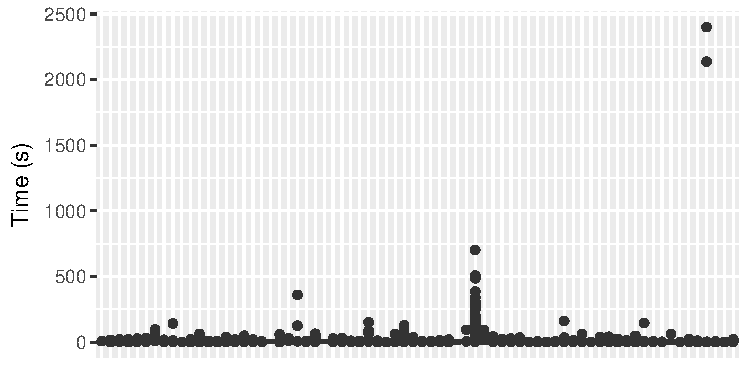
\includegraphics[width=0.5\textwidth]{R/testcost.pdf}  
%%   \caption{\label{fig:relativesd}Distribution of RSD ($\sigma/\mu$)
%%     across projects.}
%% \end{figure}

%% Figure~\ref{fig:relativesd} shows the distribution of RSD across
%% medium and long-running projects.  Results show that the distribution
%% is skewed to the right indicating that test costs are relatively well
%% distributed in most costly projects we analyzed \Fix{$\leftarrow$
%%   confirm}.

%% analyzed the execution time
%% for the \numMedLong{} projects from the \longg{} and \medg{} groups
%% (see Section~\ref{sec:rqA}).
%% For each subject we calculated the
%% relative standard deviation of the test cases: we collected the
%% elapsed time of each individual test, calculated the standard
%% deviation, and divided by the mean. \Jbc{I need to clarify the
%%   relationship "well/bad-balanced" regression test and relative
%%   standard deviation}

%% Results indicated that \Fix{...elaborate...}. \Jbc{We may identify
%% different groups of subjects}\Fix{TODO: collect data + compute the
%% statistic, create a scatter plot to identify groups of subjects}

%% Regression tests that are well distributed may benefit from
%% parallelism since more tests executes at the same time while the
%% opposite scenario may require a different approach. In the later
%% scenario, executing tests in parallel may have insignificant impact
%% since a small subset of test cases dominates the execution.}


\subsection{Adoption}
\label{sec:rqC}
\label{sec:rqE}

The dimension adoption focuses on the usage of parallelism in
open-source projects.  It evaluates (\numRQAdoptionOne) how often open-source
projects use parallelization schemes and (\numRQAdoptionTwo) how developers
involved in costly projects, not using parallelization, perceive this
technology.

\begin{itemize}
    \item \numRQAdoptionOne. \textbf{\RQAdoptionOne{}}
\end{itemize}

To answer \numRQAdoptionOne{}, we selected all projects from the \medg{} and
\longg{} groups, \ie, projects that ran in at least one minute.  This
set includes \numMedLong{} projects (see Section~\ref{sec:rqA}).  We
looked for dynamic and static manifestations of parallelism.

%% The
%% following section report results for each of these cases.

\vspace{1ex}
\subsubsection{Dynamic checking}
\label{sec:rqC-1}

To find dynamic evidence of parallelism, we ran the test suites from
our set of \numMedLong{} projects to output all key-value pairs of
Maven parameters.  To that end, we used the option~\CodeIn{-X} to
produce debug output and the option~\CodeIn{-DskipTests} to skip
execution of tests.  We skipped execution of tests as we observed from
sampling that only bootstrapping the Maven process suffices to infer
which parallel configuration modes it will use to actually run the
tests.  It is also important to point that we used the default
configurations specified in the project.  We inferred parallel
configurations by searching for certain configuration parameters in
log files. According to Maven's
documentation~\cite{maven-surefire-plugin}, a parallel configuration
depends either on (1) the parameter \CodeIn{parallel} to define the
parallelism mode within a JVM followed by the parameter
\CodeIn{threadCount} or (2) the parameter
\CodeIn{forkCount}\footnote{This parameter is named \CodeIn{forkMode}
  in old versions of Maven Surefire} to define the number of forked
JVMs.  As such, we captured, for each project, all related key-value
pairs of Maven parameters and mapped those pairs to one of the
possible parallelization modes.  For instance, if a given project
contains a module with the parameter
\CodeIn{<forkCount>1C</forkCount>}, the possible classifications are
\ForkSeq{} or \ForkParMeth{}, depending on the presence and the value
of the parameter \CodeIn{parallel}.  If the parameter
\CodeIn{parallel} is set to \CodeIn{methods} the detected mode will be
\ForkParMeth{}.  Large projects may contain several test suites
distributed on different Maven modules potentially using different
configurations.  For those cases, we collected the Maven output from
each module discarding duplicates as to avoid inflating counts for
configuration modes that appear in several modules of the same
project. For instance, if a project contains two modules using the
same configuration, we counted only one occurrence.


\begin{wrapfigure}{r}[0pt]{0pt}%0.525\linewidth
  \footnotesize
  %  \small
  \centering
  \setlength{\tabcolsep}{2.5pt}
%    \resizebox{.48\textwidth}{!}{%
    \begin{tabular}{lrr}
        \toprule
        \emph{Subject} & \emph{\# of modules} & \emph{Mode}\\%
        \midrule%
        \Comment{BounceStorage }Chaos\Comment{ HTTP Proxy} & 1/1 &  \ParClassSeqMeth{}\\%
        \Comment{Apache }Flink & 74/74 & \ForkSeq{} \\%        
        \Comment{JenkinsCI }Gerrit\Comment{ Trigger Plugin} & 1/1 & \ForkSeq{}\\%
        \Comment{Spotify }Helios & 8/8 & \ForkSeq{}\\%
        Javaslang & 3/3 & \ParClassParMeth{}\\%
        Jcabi\Comment{ Github} & 1/1 & \ParClassParMeth{}\\%        
        \Comment{Hazelcast }Jet & 7/14 & \ForkSeq{}\\%
        \Comment{Apache Logging }Log4J2 & 25/31 & \ForkSeq{}\\%
        \Comment{Jankotek }MapDB & 1/2 & \ParClassParMeth{}\\%        
        \bottomrule%
    \end{tabular}
    \caption{Subjects with parallel test execution enabled by
    default.}
    \label{tab:freqmodes-dynamic}
\end{wrapfigure}
Figure~\ref{tab:freqmodes-dynamic} shows the projects we idendified
where parallelism is enabled by default in Maven.  Column
``\emph{Subject}'' indicates the name of the project, column
``\emph{\# of modules}'' indicates the fraction of modules containing
tests that use the configuration of parallelism mentioned in column
``\emph{Mode}''.  We note that, considering these projects, the
modules that do not use the configuration cited use the sequential
configuration \Seq{}.  For example, six modules (=31-25) from Log4J2
use sequential configuration.

It came as a surprise the observation that
no project used distinct configurations in their modules. Considering
our set of \numMedLong{} projects, we found that only
\textbf{\numProjectsPar{}} of those projects had parallelism enabled
by default, with only configurations \ParClassSeqMeth{},
\ParClassParMeth{}, and \ForkSeq{} being used.  Configurations
\ParClassParMeth{} and \ForkSeq{} were the most popular among these
cases.  Note that these results under-approximate real usage of
parallelism as we used default parameters in our scripts to spawn the
Maven process.  That decision could prevent execution of particular
test modules.
%\begin{figure}[h!]
%    \centering
%    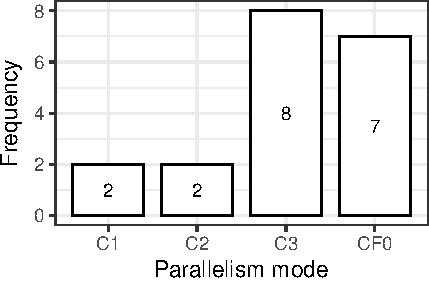
\includegraphics[width=0.32\textwidth]{plots/barplot-modes-dynamic.pdf}
%    \caption{\label{fig:freqmodes-dynamic}\Fix{fix
%    caption}Distribution of parallel modes identified dynamically in a
%    subset of \numProjectsPar{} projects.  A project may have support
%    to more than one parallel mode. Also, a project may run only a
%    subset tests in parallel by default.}
%\end{figure}

%% Recall that some projects can use parallel execution that is only
%% activated when developers pass certain parameters to the build
%% process. For instance, it is possible to create in Maven multiple
%% configurations in the same build file and select dynamically which one
%% should be used.  

\subsubsection{Static checking}
\label{sec:rqC-2}
Given the inherent limitation of dynamic monitoring to find evidence
of parallelism, we also looked for indication of parallelism in build
files\Comment{ in the same sample set of \numMedLong{} projects}.  We
parsed all \emph{pom.xml} files under the project's directory and used
the same approach as in our previous analysis to classify
configurations.  We noticed initially that our approach was unable to
infer the configuration mode for cases where the decision depends on
the input (\eg,
\CodeIn{<parallel>\$\{parallel.type\}</parallel>}). For these
projects, the tester needs to provide additional parameters in the
command line to enable parallelization (\eg, \CodeIn{mvn test
  -Dparallel.type=classesAndMethods}). To handle those case, we
considered all possible values for the parameter (in this case,
\CodeIn{\$\{parallel.type\}}).  It is also important to note that this
approach is not immune to false negatives, which can ocurr when
\emph{pom.xml} files are encapsulated in jar files or downloaded from
the network.  Consequently, this static checking is complementary to
the dynamic checking, previously presented.

Overall, we found, using this methodology, ten projects that use
parallelism.  Compared to the set of projects listed in
Figure~\ref{tab:speedup}, we found two new projects, namely:
\CodeIn{Google Cloud\Comment{ Platform} DataflowJavaSDK} (using
configuration C3) and \CodeIn{Mapstruct} (using configuration
\ForkSeq{}).  Curiously, we also found that project \CodeIn{Jcabi} was
not detected using this methodology.  That happened because this
project loads its \emph{pom.xml} file from a jar file that we did not
check.  Considering the static and dynamic methods together, we found
a total of 11 distinct projects using parallelism, corresponding to
the union of the two subject sets.

\vspace{1ex}
\begin{center}
\fbox{
  \begin{minipage}{8cm}
      \textit{Answering \numRQAdoptionOne{}:}~\emph{Results indicate that test
        suite parallelization is underused.  Overall, only
        \percentParallel{} of costly projects (11 out of \numMedLong)
        use parallelism.}
  \end{minipage}
}
\end{center}
\vspace{1ex}

%False positive can happen because of comments, for instance.  
%To eliminate the cases of false positives and also to categorize 
%true positive cases, we complemented the initial mining step with a 
%manual inspection of files.
%% settings); the second step (inspection) consists in a manual
%% inspection to confirm the presence of parallelism settings in the
%% build file and classify them according to the parallelism level.
%% Figure \Fix{removed} describes the discovery step: we list the paths
%% of all build files and filter only the files that contain any of the

%% Figure~\ref{tab:inspection-table} summarizes our results.
%% \Fix{The first column indicates the group of projects according to
%% their time cost.  The second column indicates the number of build
%% files per group.  The last column indicates the ratio of projects with
%% parallelization settings.  From the \numMedLong{} subjects, we found
%% \pomMedLong{} \pomf{} files.  The \numPomMatched{} configurations are
%% distributed across \numProjectsPar{} projects from our sample.}

%% % \emph{From these results we found that $\sim$51\% of medium and
%% % long-running projects do not use parallel features to run test
%% % suites.}\Mar{please make it consistent with research
%% % question}\Mar{explain this is over(under)-estimated...}
%% \begin{figure}[ht!]
%%     \centering
%%     \resizebox{.48\textwidth}{!}{%
%%     \begin{tabular}{llcl}
%%         \toprule
%%         Group & Subject & \# of modules & Mode\\%
%%         \midrule%
%%         Long   &JenkinsCI Gerrit Trigger Plugin& 1 & \ForkSeq\\%
%%         Medium &Bouncestorage Chaos Http Proxy & 1 & C2\\%
%%         Medium &Javaslang & 1 & C3\\%
%%         Medium &Apache Flink & 1 &\ForkSeq\\%
%%         Medium &Apache Logging Log4J2 & 3 & \ForkSeq{}\\%
%%         Medium &Google Cloud Platform DataflowJavaSDK & 1 & C3\\%
%%         Medium &Hazelcast Jet & 1 & \ForkSeq\\%
%%         Medium &Jankotek MapDB & 1 & C3\\%
%%         Medium &Mapstruct & 1 & \ForkSeq\\%
%%         Medium &Spotify Helios & 3 & \ForkSeq\\%
%%         \bottomrule%
%%     \end{tabular}}
%%     \caption{Subjects with parallelization configurations in build files.}
%%     \label{tab:inspection-table}
%% \end{figure}

%% \begin{figure}[ht!]
%%     \centering
%%     \begin{tabular*}{0.48\textwidth}{@{\extracolsep{\fill}}ccc}
%%         \toprule
%%         \multirow{2}{*}{Group} %1st row, 1st cell
%%             & \multirow{2}{*}{\# \pomf{}}
%% 	    & \# \pomf{} matched\\
%%         % 2nd row - empty cell
%%             & % empty cell
%%             & / total\\%
%%         \midrule%
%% 	Long   & \numPomLong{} & 4 / \numLong{}\\%
%% 	Medium & \numPomMed{} & 6 / \numMed{}\\%
%%         \midrule%
%%         Total % last row, first cell
%%             & \pomMedLong{}
%%             & \numProjectsPar{} / \numMedLong{}\\%
%%         \bottomrule%
%%     \end{tabular*}
%%     \caption{Presence of parallelization settings in build files: the
%%     first column indicates the group of projects according to their
%%     time cost; the second column is the subset of files with parallelization
%%     keywords; the last column indicates the ratio of projects with
%%     parallelism support.}
%%     \label{tab:inspection-table} 
%% \end{figure}
%% \Jbc{rework this... $\rightarrow$} From the \numProjectsPar{} projects
%% identified above, we investigated further the \numPomMatched{}
%% build files with parallel settings.  We analyzed the support and
%% distribution of parallel modes from this subset of projects. To
%% calculate the distribution of parallel modes, we considered only the
%% presence of the mode in at least one of the project settings.  Recall
%% that a build file may contain more than one parallel setting and a
%% project may contain several sub-modules with build files.  In case the
%% value of a parallel option is resolved dynamically (\eg, via
%% command-line argument or system variable) we compute all modes related
%% to the option. For instance, depending on the value, the
%% \CodeIn{parallel} option can be \Seq{} (\CodeIn{none}),
%% \ParClassSeqMeth{} (\CodeIn{classes}), \SeqClassParMeth{},
%% (\CodeIn{methods}), and \ParClassParMeth{} (\CodeIn{all}).
%% Figure~\Fix{fig:freqmodes-static} summarizes our findings.
%% \Fix{Missing conclusion: Fork the most used configuration}
%% \begin{figure}[h!]
%%     \centering
%%     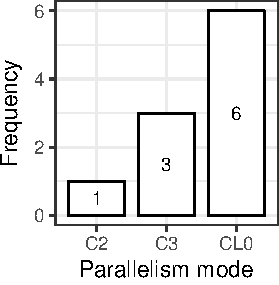
\includegraphics[width=0.32\textwidth]{plots/barplot-modes-static.pdf}
%% 	\caption{\label{fig:freqmodes-static}\Luis{This is wrong, it
%% 	should be \textbf{CF0} instead of \textbf{CL0}}Distribution of parallel modes
%%     identified statically in a subset of \numProjectsPar{} projects.
%%     A project may have support to more than one parallel mode.}
%% \end{figure}


\begin{itemize}
	\item \numRQAdoptionTwo{}. \textbf{\RQAdoptionTwo{}}
\end{itemize}

To answer this research question we surveyed developers involved in a
selection of projects from our benchmark with time-consuming test
suites.  The goal of the survey is to better comprehend developer's
attitude towards the use of parallelism as a mechanism to speedup
regression testing.  We surveyed developers from a total of
\emailsProjects{} projects.  From the initial list of \numMedLong{}
project, we discarded 11 projects that we knew a priori used
parallelization, and \discartedProjects{} projects that we could not find
developer's emails from commit logs.  From this list of projects, we
mined potential participants for our study.  More precisely, we
searched for developer's name and email from the last 20 commits to
the corresponding project repository.  Using this approach, we
identified a total of \emailsSent{} eligible participants.  Finally,
we sent plain-text e-mails, containing the survey, to those developers.  In
total, \emailsAnswered{} developers replied but we discarded
\emailsFalseAnswers{} replies with subjective answers.  Considering
projects covered by the answers, a total of \emailsProjectsAnswered{}
projects (\percEmailsProjectsAnswered{} of the total) were represented
in those replies.  Note that multiple developers on each project
received emails.  We sent the following set of questions to
developers:

\begin{enumerate}
\item How long does it take for tests to run in your environment? Can
  you briefly define your setup?
\item Do you confirm that your regression test suite does *not* run in parallel?
\item\label{questionThree} Select a reason for not using parallelization:
  \begin{enumerate}[label=\alph*)]
  \item I did not know it was possible
  \item I was concerned with concurrency issues
  \item I use a continuous integration server
  \item Some other reason. Please elaborate.
  \end{enumerate}
\end{enumerate}

%% \begin{enumerate}
%% 	\item How long does it take for test to run in your
%%		environment?
%%	\item Can you briefly define your setup?
%%	\item Do you confirm that your project does not run in
%%		parallel?
%%	\item Select a reason for not using paralellization:
%%		\begin{enumarate}
%%			\item I did not know it was possible;
%%			\item I was concerned with concurrency issues;
%%			\item I use a continuous integration server;
%%			\item Some other reason.
%%		\end{enumerate}
%% \end{enumerate}
%% One of the goals of the first questions is to identify potential
%% discrepancies between our experimental environment and the environment
%% of developers.  Overall, we found that \Fix{...}

Considering question 1, we confirmed that execution time was
compatible with the results we reported in Section~\ref{sec:rqA}.
Furthermore, \emailsCI{} of the participants indicated the use of
Continuous Integration (CI) to run tests, with \emailsDistributed{} of
these participants reporting that test suites are modularized and
those modules are tested independetly in CI servers through different
parameters.  Those participants argumented that such practice helps to
reduce time to observe test failures, which is the goal of speeding up
regression testing.  A total of \emailsLocal{} participants answered
that they do run tests in their local machines.  Note, however, that
CI does not preclude low-level parallelization.  For example,
installations of open-source CI tools (\eg{}, Jenkins~\cite{jenkins})
in dedicated servers would benefit from running tests faster through
low-level test suite parallelization.

% \emailsNotDescribed{} developers did not described their environment.

Considering question 2, the answers we collected indicated, to our
surprise, that six of the \emailsProjectsAnswered{} projects execute
tests in parallel.  This mismatch is justified by cases where neither
of our checks (static or dynamic) could detect presence of
parallelism.  A closer look at these projects revealed that one of
them contained a \emph{pom.xml} file encapsulated in a jar file
(similar case as reported in Section~\ref{sec:rqC-2}), in one of the
projects the particpant considered that distributed CI was a form of
parallelism, and in four projects the team preferred to implement
parallelization instead of using existing features from the testing
framework and the build system~---~in two projects the team
implemented concurrency control with custom JUnit test runners and in
two other projects the team implemented concurrency within test
methods.  Note that, considering these four extra cases (ignored two
distributed CI cases), the usage of parallelization increases from
\percentParallel{} to \percentParallelUpdated{}.  We do not consider
this change significant enough to modify our conclusion about
practical adoption of parallelization (\numRQAdoptionOne{}).

%% , one runs a manually created Thread to run some
%% tests, and the other runs in parallel by using Java 8 collection
%% streams, that allows the developers to iterate over a list in
%% parallel.

%% did not confirmed, however,
%% the developers confirmed the need of an extra parameter at the command
%% line to execute in parallel.

Considering question 3, the distribution of answers was as follows.  A
total of \emailsA{} of the \emailsProjectsAnswered{} developers who
answered the survey did not know that parallelism was available in
Maven (option ``a''), \emailsB{} of developers mentioned that they did
not use parallelism concerned with possible concurrency issues (option
``b''), \emailsD{} of developers mentioned that continuous integration
services sufficed to provide timely feedback while running only smoke
\begin{wrapfigure}{r}[0pt]{0pt}%0.525\linewidth
    \centering
    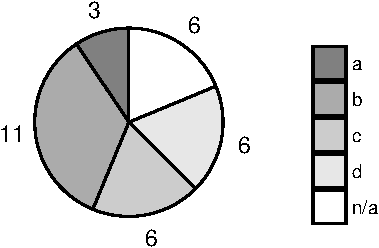
\includegraphics[width=.18\textwidth]{plots/survey.pdf}
    \caption{\label{fig:rq5-answers}Summary of developer's answers to
      survey question~\ref{questionThree}.}
\end{wrapfigure}
tests (\ie{}, short-running tests) locally (option ``c'')\Comment{here
  I want to say that they use it for something like "non-blocking
  testing" while developing in a local machine}, and \emailsD{} of
developers who provided an alternative answer (option ``d'') mentioned
that using parallelism was not worth the effort of preparing the test
suites to take advantage of available processing power.  A total of
\emailsNA{} of participants did not answer the last question of the
survey.  The pie chart in Figure~\ref{fig:rq5-answers} 
summarizes the distribution of answers.

\begin{center}
\fbox{
	\begin{minipage}{8cm}
	  \textit{Answering \numRQAdoptionTwo{}:}~\emph{Results suggest that dealing
       with concurrency issues (\ie{}, the extra work to organize test
       suite to safely explore concurrency) was the principal reason
       for developers not investing in parallelism.  Other reasons
       included availability of continuous integration services and
       unfamiliarity with the technology.}
	\end{minipage}
}
\end{center}

\subsection{Speedups}
\label{sec:rqD}

\begin{itemize}
    \item \numRQSpeedupOne{}. \textbf{\RQSpeedupOne}
\end{itemize}

To answer \numRQSpeedupOne{}, we considered the \numProjectsPar{}
subjects from our benchmark that use parallelization \emph{by default}
(see Figure~\ref{tab:freqmodes-dynamic}).  We compared running times
with parallelization~---~configured by project owners~---~and without
parallelization.

%% In those projects, parallelization is active without
%% passing any extra parameters.  Section~\ref{sec:rqC-1} describes in
%% detail the methodology we used to find these subjects.
%and
%Section~\ref{seq:rq6-tradeoffs}, we verified that both
%% executions produce the same outcome to eliminate noise from failing
%% tests.  To compute the speedup, we divide the time obtained in the
%% sequential execution by the time obtained from the default execution.
%% For instance, if a project runs the tests sequentially in $10m$ and
%% the same execution runs in $5m$ with parallelization enabled (default
%% execution), the speedup is two.

Figure~\ref{tab:speedup} summarizes results.  Lines are sorted by
project names.  Columns ``\emph{Group}'' and
``\emph{Name}'' indicate, respectively, the group and the name of the
subject.  Column ``$T_s$'' shows sequential execution time and column
``$T_p$'' shows parallel execution time. Column ``$T_s/T_p$'' shows
speedup or slowdown.  As usual, a ratio above 1x denotes speedup
and a ratio below 1x denotes slowdown.

\begin{figure}[h!]
\centering
\resizebox{.41\textwidth}{!}{%
  \scriptsize
\begin{tabular}{llrrr}
\toprule
\emph{Group} & \emph{Subject} & \multicolumn{1}{c}{$T_s$} & \multicolumn{1}{c}{$T_p$} & $T_s/T_p$ \\%
\midrule%
Medium & \Comment{BounceStorage }Chaos\Comment{ HTTP Proxy} & 1.51m & 1.47m & 
    \cellcolor{lightgray}1.01x\\%
Medium &\Comment{ Apache }Flink& 11.79m & 2.57m & 4.59x\\%
Long &\Comment{ Jenkins CI }Gerrit\Comment{ Plugin} & 51.19m & 40.31m &  1.26x\\%
Medium &\Comment{ Spotify }Helios& 4.46m & 1.63m & 2.73x\\%  
Medium &Javaslang& 2.18m & 1.82m & 1.19x\\%
Medium &Jcabi\Comment{ GitHub} & 2.76m & 0.30m &
    \cellcolor{lightgray}9.2x\\%
Medium &\Comment{ Hazelcast }Jet& 8.26m & 3.67m & 2.25x\\%
Long &\Comment{ Apache }Log4J2& 8.24m & 8.21m & \cellcolor{lightgray}1.00x\\%
Long &\Comment{ Jankotek }MapDB& 10.06m & 8.58m & 1.17x\\%
\midrule
\textbf{average} &  &  &  & \avgSpeedup{}x\\
\bottomrule%
\end{tabular}}
\caption{\label{tab:speedup}Speedup (or slowdown) of parallel
  execution ($T_p$) over sequential execution ($T_s$).  Default
  parallel configuration of Maven is used.  Highest slowdown/speedup
  appears in gray color.}
\end{figure}

Results indicate that, on average, parallel execution was
\avgSpeedup{} times faster compared to sequential execution.  Three
cases worth special attention: \CodeIn{Chaos}, \CodeIn{Jcabi} and
\CodeIn{Log4J2}.  No significant speedup was observed in
\CodeIn{Chaos}, a project with only three test classes, of which one
monopolizes the bulk of test execution time.  This project uses
configuration \ParClassSeqMeth{}, which runs test classes in parallel
and test methods, declared in each class, sequentially.  Consequently,
speedup cannot be obtained as the cost of the single expensive test
class cannot be broken down with the selected configuration.  Although
project \CodeIn{Jcabi} also uses configuration \ParClassSeqMeth{},
results obtained are very different compared to \CodeIn{Chaos}.  The
speedup observed in \CodeIn{Jcabi} was the highest amongst all
projects.  This project contains test classes with a small number of
test methods and several methods in those classes are time-consuming.
As result, the CPUs available for testing are kept occupied for the
most part during test execution.  Finally, we note that parallel
execution in \CodeIn{Log4J2} was innefective.  We found that Maven
invokes several test modules in this project but the test modules that
dominate execution time run sequentially by default.

%% The third, runs parallel configuration in
%% \Fix{80\%} of the project modules, however, the test time is dominated
%% by one of the sequentially running modules.  \Luis{$\leftarrow$ rework
%%   this} \Fix{falar sobre o resultado geral dos speedups - elaborar
%%   menor e maior speedup... acho que so vale a pena discutir quando
%%   tiver conviccao dos 2 casos}

\begin{center}
\fbox{
  \begin{minipage}{8cm}
    \textit{Answering \numRQSpeedupOne{}:}~\emph{Considering the
      machine setup we used, the average speedup observed with default
      configurations of parallelization was \avgSpeedup{}x.}
  \end{minipage}
}
\end{center}

\begin{itemize}
    \item \numRQSpeedupTwo{}. \textbf{\RQSpeedupTwo}
\end{itemize}

\newcommand{\subjectScalability}{MapDB}

This experiment evaluates the impact of making available to the build
system a growing number of CPUs for testing.  For that reason, we used
a machine with more cores compared to the one described in
Section~\ref{sec:setup}.  We used a Xeon E5-2660v2 (2.20GHz) Intel
processor machine with 80 virtual CPUs (40 cores with two native
threads each) and 256GB of memory, running Ubuntu 14.04 LTS Trusty
Tarr (64-bit version). This experiment uses configuration \ForkSeq{}
\begin{wrapfigure}{r}[0pt]{0pt}%0.525\linewidth
    \centering
    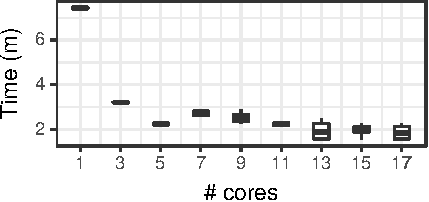
\includegraphics[width=.2\textwidth]{R/scalability/scalability.pdf}
    \caption{\label{fig:scalability}Scalability.}
\end{wrapfigure}
as the goal is to evaluate the impact on runtime of spawning a growing number of
JVMs in different CPUs.  Furthremore, we selected subject
\subjectScalability{} as it represents the case of a long-running test
suite (see Figure~\ref{tab:speedup}) with test cases distributed
across many test classes (194 test classes for \subjectScalability{}).
Note that a test class is the smallest unit that can be used to spawn
a test job on a JVM and that we have no control over which test
classes will be assigned to which JVM that the build system forks.

Figure~\ref{fig:scalability} shows the reduction of running times as
more CPUs contribute to the execution.  \Fix{elaborate...}

\begin{center}
\fbox{
  \begin{minipage}{8cm}
    \textit{Answering \numRQSpeedupTwo{}:}~\emph{...}
  \end{minipage}
}
\end{center}

\subsection{Issues}
\label{sec:rq6-tradeoffs}

This dimension assesses the impact of using distinct parallel
configurations on test flakiness (negative impact) and speedup
(positive impact).  Furthermore, note that Section~\ref{sec:rqD}
evaluated speedup in isolation, focused on projects configured to use
parallelism by default.

\begin{itemize}
    \item \numRQIssuesOne{}. \textbf{\RQIssuesOne{}}
\end{itemize}


%% The intuition is that efficiency and flakiness are inversely
%% proportional in some cases: if too many tests depends on the state of
%% a single external resource, several tests are likely to fail as the
%% degree of concurrency increases by exploiting maximum CPU usage.

%% Table header macros
% $\Uparrow_\text{speed}$
\newcommand{\subcolA}{$\text{speedup}$}
\newcommand{\subcolB}{$\%_\text{fail}$}
\newcommand{\colheader}[1]{\multicolumn{2}{c}{\emph{#1}}}
\newcommand{\blankentry}{\entry{-}{-}}
\newcommand{\subcol}{\subcolA{} & \subcolB{}}
\newcommand{\entry}[2]{#1 & #2}

\begin{figure*}[t]  
\centering
\small
\setlength{\tabcolsep}{3pt}
\begin{tabular}{l|rr|rr|rr|rr|rr|rr}
\toprule
\multirow{2}{*}{\emph{Subject (module)}} & \multicolumn{2}{c|}{\emph{\Seq}} &
    \colheader{\SeqClassParMeth} & \colheader{\ParClassSeqMeth} &
    \colheader{\ParClassParMeth} & \colheader{\ForkSeq} &
    \colheader{\ForkParMeth} \\ %\cline{2-12}
    & $T$ & $\mathit{N}$ & \subcol{} & \subcol{} & \subcol{} & \subcol{}
    & \subcol{}\\%
\midrule%
AWS SDK Java (\CodeIn{core})  & \entry{3.7m}{847}  & \entry{1.95x}{2.24\%} & \entry{2.47x}{2.77\%} & \entry{3.70x}{4.01\%} & \entry{}{} & \entry{}{}\\%

Facebook Linkbench    & \entry{4.3m}{98}  & \entry{1.00x}{0\%} & \entry{1.65x}{1.02\%} & \entry{1.59x}{1.02\%} & \entry{}{} & \entry{}{}\\%

GoogleCloud Dataflow Java (\CodeIn{sdk}) & \entry{1.6m}{3,345}  & \entry{1.23x}{1.67\%} & \entry{2.67x}{1.05\%} & \entry{0.80x}{5.35\%} & \entry{}{} & \entry{}{}\\%

Javaslang (\CodeIn{core})     & \entry{1.1m}{17,513}  & \entry{1.38x}{0\%} & \entry{1.83x}{0\%} & \entry{1.38x}{0\%} & \entry{}{} & \entry{}{}\\ 
JCabi Github                  & \entry{2.6m}{634} & \entry{2.10x}{0\%} & \entry{17.70x}{0\%} & \entry{28.80x}{0\%} & \entry{}{} & \entry{}{} \\
JCTools (\CodeIn{core})       & \entry{3.6m}{690}  & \entry{4.50x}{0\%} & \entry{3.60x}{0\%} & \entry{18.00x}{0\%} & \entry{}{} & \entry{}{}\\%
MapDB  & \entry{8.2m}{5,324}  & \entry{1.52x}{0\%} & \entry{2.73x}{0\%} & \entry{4.82x}{0.05\%}   & \entry{}{} & \entry{}{}\\%
Moquette                      & \entry{3.7m}{169} & \entry{4.62x}{65.64\%} & \entry{3.36x}{32.92\%} & \entry{12.33x}{77.78\%} & \entry{}{} & \entry{}{} \\
RipMe                         & \entry{1.1m}{54}  & \entry{0.94x}{0\%} & \entry{1.63x}{0\%} & \entry{1.63x}{0\%} & \entry{1.37x}{0\%} & \entry{1.42x}{0\%}\\
Stripe Java     & \entry{4.3m}{302}  & \entry{4.78x}{6.31\%} & \entry{3.31x}{7.31\%} & \entry{21.50x}{14.95\%} & \entry{}{} & \entry{}{}\\%





\midrule

\textbf{Average}   & \entry{-}{-} & \entry{-}{-} & \entry{-}{-} & \entry{-}{-}
& \entry{-}{-} & \entry{-}{-} \\%


%%  & \entry{x.xm}{0}  & \entry{}{\%} & \entry{}{\%} & \entry{}{\%} & \entry{}{} & \entry{}{}\\%
%%OpenMRS Core (\CodeIn{api})  & \entry{15.4m}{3436} & \blankentry{}        & \blankentry{}        & \blankentry{} & \entry{1.5x}{0\%} & \entry{1.7x}{0}\\%
%%Apache Flume (\CodeIn{core}) &  \entry{7.7m}{392}  & \blankentry{}        & \blankentry{}        & \blankentry{}       & \entry{0.9x}{0\%} & \blankentry{} \\%
%%Facebook Archive Linkbench   &  \entry{4.5m}{98}   & \entry{1.0x}{0.2\%}  & \entry{1.6x}{1.2\%}       & \entry{1.0x}{0\%}  & \entry{1.7x}{0.5\%}  & \entry{1.7x}{0.2\%}\\%
%%AWS SDK Java (\CodeIn{core}) &  \entry{3.8m}{847}  & \multicolumn{6}{c}{\Fix{requires investigation}} & \entry{2.2x}{0.1\%} & \entry{3.2x}{2.0\%}\\%

%% OpenMRS Core (\CodeIn{api})  & \entry{15.4m}{3436} & \blankentry{}        & \blankentry{}        & \blankentry{} & \entry{1.5x}{0\%} & \entry{1.7x}{0}\\%
%% Jankotek MapDB               &  \entry{9.9m}{5218} & \multicolumn{6}{c}{\cellcolor{lightgray}\emph{JVM Crash}} & \entry{1.5x}{0\%} & \entry{1.7x}{0\%}\\%
%% Apache Flume (\CodeIn{core}) &  \entry{7.7m}{392}  & \blankentry{}        & \blankentry{}        & \blankentry{}       & \entry{0.9x}{0\%} & \blankentry{} \\%
%% Apache Giraph (\CodeIn{core})&  \entry{7.2m}{236}  & \entry{2.1x}{5.1\%}  & \colheader{\cellcolor{lightgray}timeout}   & \entry{1.0x}{0\%} & \entry{1.0x}{0}\% & \colheader{\cellcolor{lightgray}JVM Crash}\\%
%% Facebook Archive Linkbench   &  \entry{4.5m}{98}   & \entry{1.0x}{0.2\%}  & \entry{1.6x}{1.2\%}       & \entry{1.0x}{0\%}  & \entry{1.7x}{0.5\%}  & \entry{1.7x}{0.2\%}\\%
%% Stripe Java                  &  \entry{4.2m}{302}  & \entry{4.2x}{5.2\%}  & \entry{3.5x}{5.7\%}       & \entry{4.2x}{6.3\%} & \entry{1.0x}{0.3\%} & \entry{4.2x}{5.7\%}\\%
%% AWS SDK Java (\CodeIn{core}) &  \entry{3.8m}{847}  & \multicolumn{6}{c}{\Fix{requires investigation}} & \entry{2.2x}{0.1\%} & \entry{3.2x}{2.0\%}\\%

%% Jenkins CI Github            & \entry{Xm}{Z}       & \entry{x}{\%}          & \entry{x}{\%} & \entry{x}{\%} & \entry{x}{\%} & \entry{x}{\%}\\%
%% Jenkins CI Docker Workflow   & \entry{Xm}{Z}       & \entry{x}{\%}          & \entry{x}{\%} & \entry{x}{\%} & \entry{x}{\%} & \entry{x}{\%}\\%
%% Hazelcast                    & \entry{Xm}{Z}       & \entry{x}{\%}          & \entry{x}{\%} & \entry{x}{\%} & \entry{x}{\%} & \entry{x}{\%}\\%

\bottomrule%
\end{tabular}
\caption{Speedup versus Flakiness (\subcolB). Configuration
  \emph{\Seq{}} denotes the comparison baseline, which runs tests
  sequentially.  Columns $T$ and $N$ indicate time and number of
  tests, respectively.  Other columns show speedup and percentage of
  failing tests in different configurations, compared to
  \emph{\Seq{}}.\Mar{Can you please add name of module for all subjects?}}
\label{tab:rq6-table}
\end{figure*}

To answer this research question, we conducted an experiment involving
the six parallel configurations from Section~\ref{sec:modes}  and the
top 10 long-running test modules from our sample set. The rationale
for this selection criteria was to maximize the chances of observing
speedup and flakiness, assuming that long-running tests also have many
tests. Indeed, we confirmed that test suites in these projects contain
at least 236 tests ($1,662.7$ in average). Also, we preferred to compare the
effect of a configuration over a single test module for projects with
multiple test modules.  Recall that large projects may contain several
test modules, and these modules may contain distinct characteristics
that could favor one configuration and not others; therefore, it would
be necessary to check each module individually for a fair comparison.
We are interested in understanding how efficiency (\ie, testing cost)
and flakiness (\ie, failing tests) are affected when we run a test
suite with different parallel configurations.  Recall that increased
resource contention obtained with parallelism can lead to concurrency
issues such as data races.  Flakiness and speedup are contradictory
forces that drive configuration selection.  We used as a \emph{control
group} (\ie, baseline) the sequential execution of each subject's
tests. Notice that for measuring flakiness, we have to consider only
tests that failed due to the concurrency in the parallel execution.
For that reason, we re-executed the tests in sequence ten times and
carefully verified that there are only passing tests in our baseline.
We considered ten as the number of re-executions based on the approach
used by Google reported in a previous work on test
flakiness~\cite{luo-etal-fse2014}.  To obtain parallel configurations,
we implemented a script that takes a subject and a configuration (\eg,
\ForkSeq{}) as inputs, and the script outputs the modified version of
the subject with the desired configuration. The workflow consists in
copying the project directory to a new directory, finding all existing
build files (\ie, \pomf{} files), and modifying all existing Maven
Surefire configurations with new values for the parameters
\CodeIn{parallel}, \CodeIn{forkCount}, and \CodeIn{threadCount} using
an XPath~\cite{xpath} library to manipulate XML documents. For
configurations with forked JVMs enabled (\ie, \ForkSeq{} and
\ForkParMeth{}), we changed the \CodeIn{forkCount} with the value
\CodeIn{1C} (\ie, one JVM per core).  To adjust the pool of threads
for parallelism within a JVM, we changed the parameter
\CodeIn{threadCount} with \Jbc{should we consider 2 as it is the
number of native threads per core OR 6 as it represents 3 Cores * 2
native threads?}.  To run the subjects and their respective variations
(\ie, the modified versions according to the parallelism
configuration), we used a similar approach as described in


Figure~\ref{fig:mvn-execution} except that we added a timeout of one
hour to run the tests. We used the \CodeIn{timeout}
command~\cite{timeout-cmd} to monitor the execution, and we configured
the command to dispatch a \emph{kill} signal if the test execution
exceeds the time limit. We imposed this time constraint to avoid
hanging indefinitely the experiment execution due to some thread
contention that may occur (\eg, deadlock). Finally, we saved each
execution log and XML test reports generated by Maven to collect the
execution time, the number of failing tests, and for reference to
analyze and diagnose outliers in our results. For efficiency, we
reported the speedup (\ie, $\Uparrow_\text{speed} = T_{\text{s}} /
T_{\text{p}}$) in average, and for flakiness, we reported the rate of
failing tests (\ie, $\mathit{\%_\text{fail} = failures / tests}$) in
average.  Figure~\ref{tab:rq6-table} summarizes the obtained results
ordered by the time cost (\ie, $T_\text{cost}$). \Fix{Remember to
explain efficiency cutoff, JVM crashes and timeout}

\Jbc{Lembrar que investigar o slowdown de Dataflow... os logs indicam que varios
dos testes que quebraram tentavam fazer uma autenticacao em algum servico.
Possivelmente o slowdown se deve ao tempo de resposta do servico quando
a autentiticao falha}

%% \begin{figure}[h!]
%% \centering
%% \resizebox{.48\textwidth}{!}{%
%% \begin{tabular}{lcrrrrr}
%% \toprule
%% \emph{Subject} & \emph{\# of tests} & \emph{\SeqClassParMeth{}} & \emph{\ParClassSeqMeth{}} & \emph{\ParClassParMeth{}} & \emph{\ForkSeq{}} & \emph{\ForkParMeth{}}\\%
%% \midrule%
%% Linkedin Pinot & 356 & - & - & - & - & -\\%
%% %% Jenkins CI Github Plugin & - & - & - & - & 0\% & -\\%
%% %% Kite SDK & - & - & - & - & - & -\\%
%% %% \Fix{!?} Apache Giraph & 327 & - & - & - & - & -\\%
%% %% OpenMRS Core & - & - & - & - & - & -\\%
%% %% Jenkins CI Docker Workflow Plugin & - & - & - & - & 0\% & -\\%
%% %% \Fix{Flaky} Apache Eagle & - & - & - & - & - & -\\%
%% %%Geotools & 7701 & - & - & - & - & -\\%
%% %%Kuromoji & 672 & - & - & - & - & -\\%
%% %%Atomix & 99 & - & - & - & - & -\\%
%% %%\Fix{Snazy OHC} & - & - & - & - & - & -\\%
%% %%\Fix{RoaringBitmap} & - & - & - & - & - & -\\%
%% \bottomrule%
%% \end{tabular}}
%% \caption{\Fix{Tabela de flakiness}}
%% \label{tab:rq6-flaky}
%% \end{figure}

\Fix{Elaborate results from efficiency}

\Fix{Elaborate results from flakiness}

\Fix{highlight special cases}

\Fix{Draw conclusions}

\begin{center}
\fbox{
\begin{minipage}{8cm}
\textit{Answering \numRQIssuesOne{}:~\emph{\Jbc{summarize findings...}}}
\end{minipage}
}
\end{center}

%%  LocalWords:  RQ occurence parallelization Tradeoffs API readme th
%%  LocalWords:  mvn clearcut escapeinside xleftmargin untestable LTS
%%  LocalWords:  framexleftmargin CPUs Tahr sysstat gh Vagrantfile
%%  LocalWords:  javadoc isolcpus JUnit's JUnitCore Gligoric boxplots
%%  LocalWords:  outliers apache uber chaperone facebookarchive
%%  LocalWords:  linkbench priori


We ran the test suite for each subject three times, reporting averaged
execution times in three ranges: tests that run within a minute
(\shortg{} group), tests that run in one to five minutes (\medg{}
group), and tests that run in five or more minutes (\longg{}
group). We followed a similar methodology to group projects by time as
Gligoric~\etal{}~\cite{gligoric-etal-issta2015} in their work on
regression test selection.\Comment{ and added the \medg{} group due to
  the variability of the time cost from subjects out of the \shortg{}
  group} Figure~\ref{fig:rq1-barplot} shows the number of projects in
each group.  As expected, \longg{} and \medg{} projects do not occur
as frequently as \shortg{} projects.  However, they do occur in
relatively high numbers.

Figure~\ref{fig:rq1-boxplot} shows cost distribution of test suites in
each group as boxplots.  Note that the y-ranges are different.  The
distribution associated with the \shortg{} group is the most
unbalanced (right skewed)\Comment{ with outliers closed to the \medg{}
  group}.  The test suites in this group ran in 15 or less seconds for
over 75\% of the cases.  Such scenarios constitute the majority of the
cases we analyzed.  Considering the groups \medg{} and \longg{},
however, we found many costly executions.  Nearly 75\% of the projects
from the \medg{} group take over 3.5 minutes to run and nearly 75\% of
the projects from the \longg{} group take $\sim$20 minutes to run.  We
found cases in the \longg{} group were execution takes over 50 minutes
to complete, as can be observed from the outliers (dots) in the plot.

%% the median from the
%% \medg{} group is nearly two minutes and most of the subjects run in
%% less than four minutes; most of the \longg{} group runs in less than
%% 25 minutes but has outliers that require more than 50 minutes to
%% execute.



\begin{figure}[ht]
    \centering
    \begin{subfigure}{0.182\textwidth}
        \centering
        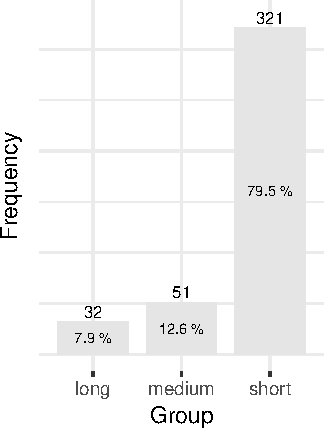
\includegraphics[width=\textwidth]{plots/barplot-timecost.pdf}
        \caption{\label{fig:rq1-barplot}}
    \end{subfigure}%
    ~
    \begin{subfigure}{0.25\textwidth}
        \centering
        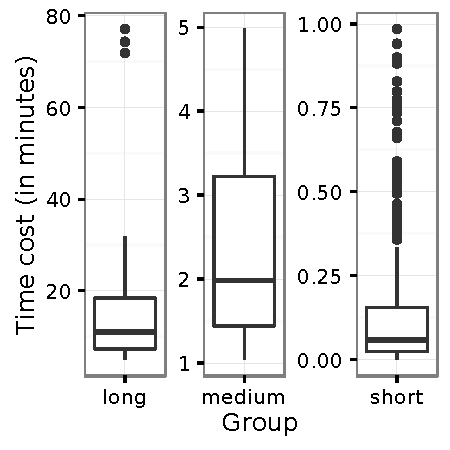
\includegraphics[width=\textwidth]{plots/boxplot-timecost.pdf}
        \caption{\label{fig:rq1-boxplot}}
    \end{subfigure}%
    \caption{(a) Subjects grouped by time cost ($t$): short run ($t <
    1m$), medium run ($1m \le t < 5m$), and long run ($5m \le t$); (b)
    Distribution of time cost by group.}
\end{figure}

%% Figure~\ref{fig:rq1-barplot} is a lower bound estimation of cost
%% because some tests may finish earlier than expected due to existing
%% test failures in the revision we downloaded.

It is important to note that we under-estimated cost in our
experiments for two main reasons.  First, some tests may finish
earlier than expected due to the observed test failures in some of the
revisions we downloaded.  From the \numSubjs{} testable projects,
\numSubjsPass{} successfully executed all tests and \numSubjsFail{}
reported some test failures.  Second, some projects may omit
long-running tests on their default execution. For instance, the
project \CodeIn{apache.maven-surefire} runs all unit tests in a few
seconds.  According to our criteria, this project is to be classified
as \shortg{} but a closer look reveals that only smoke tests are run
by default in this project.  Time-consuming integration and system
tests are only accessible via custom parameters, which we do not
handle in our experimental setup.  We enabled such parameters for this
specific project and observed that testing time goes to nearly 30
minutes.  For simplicity, we considered only the tests executed by
default.

\vspace{1ex}
\begin{center}
\fbox{
\begin{minipage}{8cm}
    \textit{Answering \numRQFeasibilityOne{}:}~\emph{We conclude that
      time-consuming test suites are relatively frequent in
      open-source projects.  We found that \percentMedLongRunning{} of
      the \numSubjs{} projects we analyzed (\ie{}, over 1 in every 5
      projects) take at least 3 minutes to run and
      \percentLongRunning{} take at least 5 minutes to run.\Comment{
        (\ie, \numMedLong{} projects from \medg{} and \longg{}).}}
\end{minipage}
}
\end{center}
\vspace{1ex}


\begin{itemize}
    \item \numRQFeasibilityTwo. \textbf{\RQFeasibilityTwo}
\end{itemize}

Section~\ref{sec:rqA} showed that medium and long-running projects are
not uncommon, accounting to nearly \percentMedLongRunning{} of the
\numSubjs{} projects we analyzed.  Research question \numRQFeasibilityTwo{}
measures the distribution of test costs in test suites as to estimate
(lack of) potential of obtaining speedups with parallelization.  In
the limit, if cost is dominated by a single test from a large test
suite, it is unlikely that parallelization will be beneficial as a
test method is the smallest working unit in test frameworks.

%% However, avoiding
%% frequent context switches is another factor to consider.  For example,
%% assuming there are at least two CPUs available for execution, cost can
%% be cut in half if two tests in a large test suite dominate execution
%% time and these tests are assigned to different CPUs.

%% It is therefore important to
%% speedup regressing testing in open-source projects.\Comment{not only
%%   to huge projects as those from Google~\cite{google-tap,google-ci}
%%   and Microsoft~\cite{prasad-shulte-ieee-microsoft-ci}.}



%% For the case
%% where cost is distributed more evenly across test cases, one expects
%% that speedups will be a function of the number of cores.
%% These contradictory forces, pushing number of tests and cost
%% of each test up and down, make prediction of effectiveness challenging.

\begin{figure}[h]
    \centering
    \begin{subfigure}{0.47\textwidth}
      \centering
      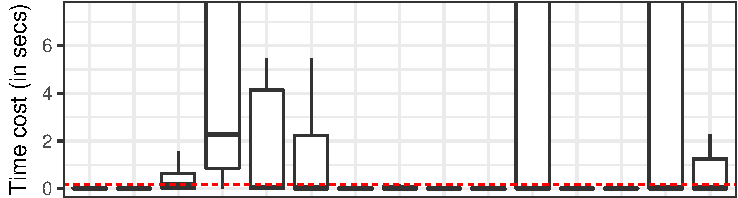
\includegraphics[width=\textwidth]{plots/testcost-long.pdf}
      \caption{\label{fig:longtcost}Long group.}
    \end{subfigure}\\
    \vspace{2ex}
    \begin{subfigure}{0.47\textwidth}
      \centering
      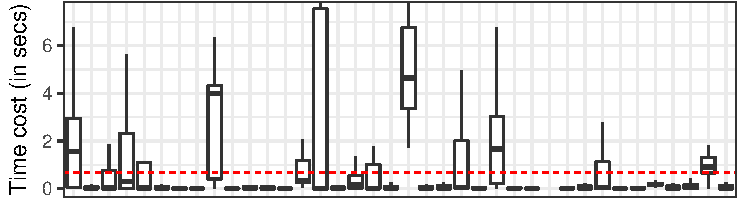
\includegraphics[width=\textwidth]{plots/testcost-medium.pdf}
      \caption{\label{fig:medtcost}Medium group.}
    \end{subfigure}
    %% \vspace{2ex}
    %% \begin{subfigure}{0.5\textwidth}
    %%   \centering
    %%   \begin{tabular}{rrrr}
    %%     \toprule
    %%     & $\sigma\leq1$ & $1<\sigma\leq5$ & $\sigma\ge5$ \\
    %%     \midrule    
    %%     Long   &  7 & 15 & 12 \\
    %%     Medium & 22 & 19 & 7 \\
    %%     \bottomrule
    %%   \end{tabular}
    %%   \caption{\label{fig:sd}Standard deviation ($\sigma$) of test case running times.}
    %% \end{subfigure}
    \caption{\label{fig:time-distributions}Time distributions.}%
\end{figure}

\sloppy Figures~\ref{fig:longtcost} and~\ref{fig:medtcost} show the
time distribution of individual test cases per project.  We observed
that the average median value of execution cost for a test was
relatively small (dashed horizontal red lines), namely 0.31s for
\medg{} projects and 0.23s for \longg{} projects.  The standard
deviations associated with each distribution were relatively
low.\Comment{ Figure~\ref{fig:sd} shows the number of projects within
  specific ranges of $\sigma$ values.}  We noted a small number of
cases of CPU monopolization.  For example, the highest value of
$\sigma$ occurred in \CodeIn{uber\_chaperone}, a project from the
medium group.  This project contains only 65 tests, 62 of which take
less than 0.5s to run, one of which takes nearly 3s to run, and two of
which take $\sim$40m to run.  For this project, 99.2\% of the
execution cost is dominated by only 3\% of the tests; without these
two costly tests this project would have been classified as
short-running.  A closer inspection in the data indicates that the
project \CodeIn{uber\_chaperone} was a corner case; we did not find
other projects with such extreme time monopolization profile.  Project
\CodeIn{facebookarchive\_linkbench} is also classified as long-running
and has the second highest value of $\sigma$.  For this project,
however, cost is distributed more smoothly across \Fix{529} tests, of
which \Fix{119 (23\%)} take more than \Fix{1s} to run with the rest of
the tests running faster.

\begin{figure}[t]
  \centering
  \begin{subfigure}{0.15\textwidth}
    \centering
    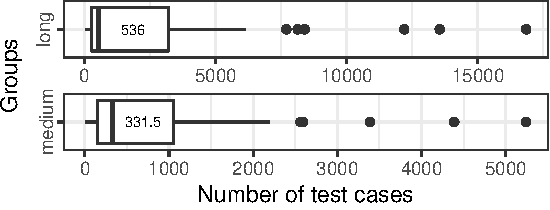
\includegraphics[width=.85\textwidth]{plots/boxplots-testcases.pdf}
    \caption{\label{fig:size-testsuites}Size of test suites.}
  \end{subfigure}
  ~
  \begin{subfigure}{0.3\textwidth}
    \centering
    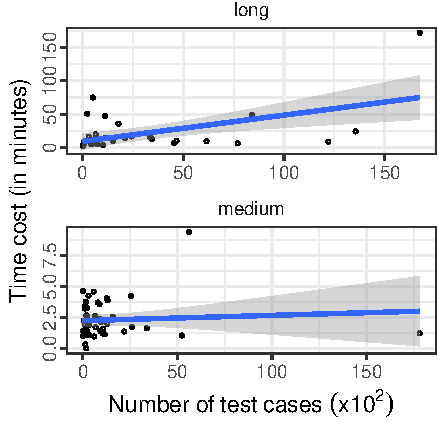
\includegraphics[width=.95\textwidth]{plots/scatter-testcost.pdf}
    \caption{\label{fig:scattercost}Size versus running time of
      test suites.}
  \end{subfigure}
  \caption{\label{fig:time-versus-size}Relating size and time.}%
\end{figure}

%\Mar{$\leftarrow$ show stats to indicate discrimination of
%  two distributions}

Figure~\ref{fig:time-distributions} showed that the average median
times were similar for \medg{} and \longg{}-running test suites.
Results indicate that the difference in overall running times of
projects in those groups was mainly justified by the number of test
cases as opposed to the individual costs of test cases.
Figure~\ref{fig:size-testsuites} shows the difference in the
distribution of test suite sizes across groups.  This figure indicates
that long projects, albeit having a wider inter-quartile range (middle
50\% projects in this group are less predictable), have a higher
median and much higher average number of test cases.  Furthermore, we
noted a strong positive correlation between running time and number of
test on projects in the \longg{} group.  Considering the \medg{}
group, the correlation between these two variables was weak.
Figure~\ref{fig:scattercost} illustrates this correlation.

%% however, weak in
%% the suggesting that saving time in this group with test suite
%% parallelization may be more challenging as relatively fewer tests
%% dominate overall execution time.  Figure~\ref{fig:scattercost} shows
%% these results.

%% This 
%% indication that it is more beneficial to parallelize long projects as
%% cost is spread across many

\vspace{1ex}
\begin{center}
\fbox{
\begin{minipage}{8cm}
    \textit{Answering \numRQFeasibilityTwo{}:}~\emph{Overall, results indicate that
    projects with a very small number of tests monopolizing end-to-end
    execution time were rare.}
\end{minipage}
}
\end{center}
\vspace{1ex}

%% We are interested to know whether
%% most of the execution cost of a subject is dominated by a small subset
%% of test cases or if the cost is nearly equally distributed. 

%% We also evaluated the dispersion of time distributions (one
%% distribution per project) to answer research question \numRQFeasibilityTwo{}.  To
%% measure dispersion \emph{across} projects we used Relative Standard
%% Deviation (RSD)~\cite{everitt-book-stats-2010}.  Note that, if we were
%% to analyze each project in isolation, the standard deviation of a
%% distribution ($\sigma$) would suffice to quantify how dispersed the
%% (time) distribution is.  However, in our case, we would like to be
%% able to compare and summarize dispersion across projects.  The RSD,
%% which is obtained dividing the standard deviation by the mean ($\mu$)
%% of a distribution, provides such normalization effect.  This metric
%% provides a lower bound (zero) but not an upper bound (somewhere close
%% to 1).  The smaller (larger) the value of RSD the more (less) uniform
%% the distribution is.  Consequently, the lower the value of RSD the
%% more parallelizable a test suite should be.

%% \begin{figure}[h!]
%%   \centering
%%   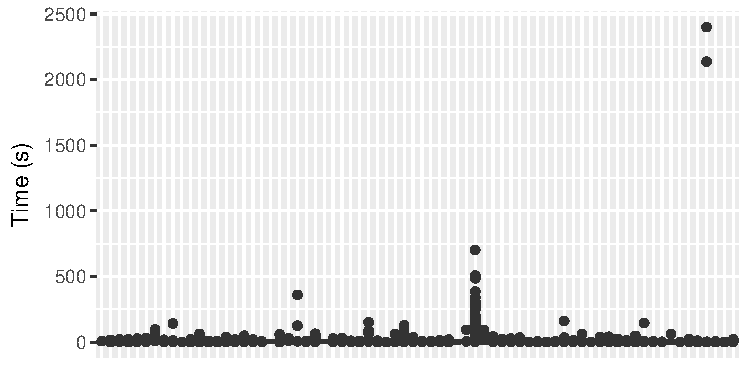
\includegraphics[width=0.5\textwidth]{R/testcost.pdf}  
%%   \caption{\label{fig:relativesd}Distribution of RSD ($\sigma/\mu$)
%%     across projects.}
%% \end{figure}

%% Figure~\ref{fig:relativesd} shows the distribution of RSD across
%% medium and long-running projects.  Results show that the distribution
%% is skewed to the right indicating that test costs are relatively well
%% distributed in most costly projects we analyzed \Fix{$\leftarrow$
%%   confirm}.

%% analyzed the execution time
%% for the \numMedLong{} projects from the \longg{} and \medg{} groups
%% (see Section~\ref{sec:rqA}).
%% For each subject we calculated the
%% relative standard deviation of the test cases: we collected the
%% elapsed time of each individual test, calculated the standard
%% deviation, and divided by the mean. \Jbc{I need to clarify the
%%   relationship "well/bad-balanced" regression test and relative
%%   standard deviation}

%% Results indicated that \Fix{...elaborate...}. \Jbc{We may identify
%% different groups of subjects}\Fix{TODO: collect data + compute the
%% statistic, create a scatter plot to identify groups of subjects}

%% Regression tests that are well distributed may benefit from
%% parallelism since more tests executes at the same time while the
%% opposite scenario may require a different approach. In the later
%% scenario, executing tests in parallel may have insignificant impact
%% since a small subset of test cases dominates the execution.}


\subsection{Adoption}
\label{sec:rqC}
\label{sec:rqE}

The dimension adoption focuses on the usage of parallelism in
open-source projects.  It evaluates (\numRQAdoptionOne) how often open-source
projects use parallelization schemes and (\numRQAdoptionTwo) how developers
involved in costly projects, not using parallelization, perceive this
technology.

\begin{itemize}
    \item \numRQAdoptionOne. \textbf{\RQAdoptionOne{}}
\end{itemize}

To answer \numRQAdoptionOne{}, we selected all projects from the \medg{} and
\longg{} groups, \ie, projects that ran in at least one minute.  This
set includes \numMedLong{} projects (see Section~\ref{sec:rqA}).  We
looked for dynamic and static manifestations of parallelism.

%% The
%% following section report results for each of these cases.

\vspace{1ex}
\subsubsection{Dynamic checking}
\label{sec:rqC-1}

To find dynamic evidence of parallelism, we ran the test suites from
our set of \numMedLong{} projects to output all key-value pairs of
Maven parameters.  To that end, we used the option~\CodeIn{-X} to
produce debug output and the option~\CodeIn{-DskipTests} to skip
execution of tests.  We skipped execution of tests as we observed from
sampling that only bootstrapping the Maven process suffices to infer
which parallel configuration modes it will use to actually run the
tests.  It is also important to point that we used the default
configurations specified in the project.  We inferred parallel
configurations by searching for certain configuration parameters in
log files. According to Maven's
documentation~\cite{maven-surefire-plugin}, a parallel configuration
depends either on (1) the parameter \CodeIn{parallel} to define the
parallelism mode within a JVM followed by the parameter
\CodeIn{threadCount} or (2) the parameter
\CodeIn{forkCount}\footnote{This parameter is named \CodeIn{forkMode}
  in old versions of Maven Surefire} to define the number of forked
JVMs.  As such, we captured, for each project, all related key-value
pairs of Maven parameters and mapped those pairs to one of the
possible parallelization modes.  For instance, if a given project
contains a module with the parameter
\CodeIn{<forkCount>1C</forkCount>}, the possible classifications are
\ForkSeq{} or \ForkParMeth{}, depending on the presence and the value
of the parameter \CodeIn{parallel}.  If the parameter
\CodeIn{parallel} is set to \CodeIn{methods} the detected mode will be
\ForkParMeth{}.  Large projects may contain several test suites
distributed on different Maven modules potentially using different
configurations.  For those cases, we collected the Maven output from
each module discarding duplicates as to avoid inflating counts for
configuration modes that appear in several modules of the same
project. For instance, if a project contains two modules using the
same configuration, we counted only one occurrence.


\begin{wrapfigure}{r}[0pt]{0pt}%0.525\linewidth
  \footnotesize
  %  \small
  \centering
  \setlength{\tabcolsep}{2.5pt}
%    \resizebox{.48\textwidth}{!}{%
    \begin{tabular}{lrr}
        \toprule
        \emph{Subject} & \emph{\# of modules} & \emph{Mode}\\%
        \midrule%
        \Comment{BounceStorage }Chaos\Comment{ HTTP Proxy} & 1/1 &  \ParClassSeqMeth{}\\%
        \Comment{Apache }Flink & 74/74 & \ForkSeq{} \\%        
        \Comment{JenkinsCI }Gerrit\Comment{ Trigger Plugin} & 1/1 & \ForkSeq{}\\%
        \Comment{Spotify }Helios & 8/8 & \ForkSeq{}\\%
        Javaslang & 3/3 & \ParClassParMeth{}\\%
        Jcabi\Comment{ Github} & 1/1 & \ParClassParMeth{}\\%        
        \Comment{Hazelcast }Jet & 7/14 & \ForkSeq{}\\%
        \Comment{Apache Logging }Log4J2 & 25/31 & \ForkSeq{}\\%
        \Comment{Jankotek }MapDB & 1/2 & \ParClassParMeth{}\\%        
        \bottomrule%
    \end{tabular}
    \caption{Subjects with parallel test execution enabled by
    default.}
    \label{tab:freqmodes-dynamic}
\end{wrapfigure}
Figure~\ref{tab:freqmodes-dynamic} shows the projects we idendified
where parallelism is enabled by default in Maven.  Column
``\emph{Subject}'' indicates the name of the project, column
``\emph{\# of modules}'' indicates the fraction of modules containing
tests that use the configuration of parallelism mentioned in column
``\emph{Mode}''.  We note that, considering these projects, the
modules that do not use the configuration cited use the sequential
configuration \Seq{}.  For example, six modules (=31-25) from Log4J2
use sequential configuration.

It came as a surprise the observation that
no project used distinct configurations in their modules. Considering
our set of \numMedLong{} projects, we found that only
\textbf{\numProjectsPar{}} of those projects had parallelism enabled
by default, with only configurations \ParClassSeqMeth{},
\ParClassParMeth{}, and \ForkSeq{} being used.  Configurations
\ParClassParMeth{} and \ForkSeq{} were the most popular among these
cases.  Note that these results under-approximate real usage of
parallelism as we used default parameters in our scripts to spawn the
Maven process.  That decision could prevent execution of particular
test modules.
%\begin{figure}[h!]
%    \centering
%    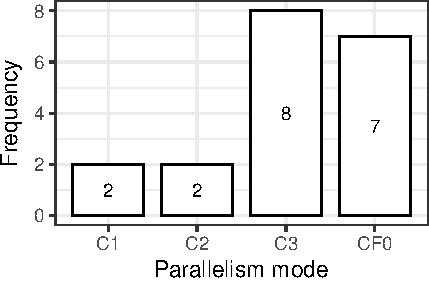
\includegraphics[width=0.32\textwidth]{plots/barplot-modes-dynamic.pdf}
%    \caption{\label{fig:freqmodes-dynamic}\Fix{fix
%    caption}Distribution of parallel modes identified dynamically in a
%    subset of \numProjectsPar{} projects.  A project may have support
%    to more than one parallel mode. Also, a project may run only a
%    subset tests in parallel by default.}
%\end{figure}

%% Recall that some projects can use parallel execution that is only
%% activated when developers pass certain parameters to the build
%% process. For instance, it is possible to create in Maven multiple
%% configurations in the same build file and select dynamically which one
%% should be used.  

\subsubsection{Static checking}
\label{sec:rqC-2}
Given the inherent limitation of dynamic monitoring to find evidence
of parallelism, we also looked for indication of parallelism in build
files\Comment{ in the same sample set of \numMedLong{} projects}.  We
parsed all \emph{pom.xml} files under the project's directory and used
the same approach as in our previous analysis to classify
configurations.  We noticed initially that our approach was unable to
infer the configuration mode for cases where the decision depends on
the input (\eg,
\CodeIn{<parallel>\$\{parallel.type\}</parallel>}). For these
projects, the tester needs to provide additional parameters in the
command line to enable parallelization (\eg, \CodeIn{mvn test
  -Dparallel.type=classesAndMethods}). To handle those case, we
considered all possible values for the parameter (in this case,
\CodeIn{\$\{parallel.type\}}).  It is also important to note that this
approach is not immune to false negatives, which can ocurr when
\emph{pom.xml} files are encapsulated in jar files or downloaded from
the network.  Consequently, this static checking is complementary to
the dynamic checking, previously presented.

Overall, we found, using this methodology, ten projects that use
parallelism.  Compared to the set of projects listed in
Figure~\ref{tab:speedup}, we found two new projects, namely:
\CodeIn{Google Cloud\Comment{ Platform} DataflowJavaSDK} (using
configuration C3) and \CodeIn{Mapstruct} (using configuration
\ForkSeq{}).  Curiously, we also found that project \CodeIn{Jcabi} was
not detected using this methodology.  That happened because this
project loads its \emph{pom.xml} file from a jar file that we did not
check.  Considering the static and dynamic methods together, we found
a total of 11 distinct projects using parallelism, corresponding to
the union of the two subject sets.

\vspace{1ex}
\begin{center}
\fbox{
  \begin{minipage}{8cm}
      \textit{Answering \numRQAdoptionOne{}:}~\emph{Results indicate that test
        suite parallelization is underused.  Overall, only
        \percentParallel{} of costly projects (11 out of \numMedLong)
        use parallelism.}
  \end{minipage}
}
\end{center}
\vspace{1ex}

%False positive can happen because of comments, for instance.  
%To eliminate the cases of false positives and also to categorize 
%true positive cases, we complemented the initial mining step with a 
%manual inspection of files.
%% settings); the second step (inspection) consists in a manual
%% inspection to confirm the presence of parallelism settings in the
%% build file and classify them according to the parallelism level.
%% Figure \Fix{removed} describes the discovery step: we list the paths
%% of all build files and filter only the files that contain any of the

%% Figure~\ref{tab:inspection-table} summarizes our results.
%% \Fix{The first column indicates the group of projects according to
%% their time cost.  The second column indicates the number of build
%% files per group.  The last column indicates the ratio of projects with
%% parallelization settings.  From the \numMedLong{} subjects, we found
%% \pomMedLong{} \pomf{} files.  The \numPomMatched{} configurations are
%% distributed across \numProjectsPar{} projects from our sample.}

%% % \emph{From these results we found that $\sim$51\% of medium and
%% % long-running projects do not use parallel features to run test
%% % suites.}\Mar{please make it consistent with research
%% % question}\Mar{explain this is over(under)-estimated...}
%% \begin{figure}[ht!]
%%     \centering
%%     \resizebox{.48\textwidth}{!}{%
%%     \begin{tabular}{llcl}
%%         \toprule
%%         Group & Subject & \# of modules & Mode\\%
%%         \midrule%
%%         Long   &JenkinsCI Gerrit Trigger Plugin& 1 & \ForkSeq\\%
%%         Medium &Bouncestorage Chaos Http Proxy & 1 & C2\\%
%%         Medium &Javaslang & 1 & C3\\%
%%         Medium &Apache Flink & 1 &\ForkSeq\\%
%%         Medium &Apache Logging Log4J2 & 3 & \ForkSeq{}\\%
%%         Medium &Google Cloud Platform DataflowJavaSDK & 1 & C3\\%
%%         Medium &Hazelcast Jet & 1 & \ForkSeq\\%
%%         Medium &Jankotek MapDB & 1 & C3\\%
%%         Medium &Mapstruct & 1 & \ForkSeq\\%
%%         Medium &Spotify Helios & 3 & \ForkSeq\\%
%%         \bottomrule%
%%     \end{tabular}}
%%     \caption{Subjects with parallelization configurations in build files.}
%%     \label{tab:inspection-table}
%% \end{figure}

%% \begin{figure}[ht!]
%%     \centering
%%     \begin{tabular*}{0.48\textwidth}{@{\extracolsep{\fill}}ccc}
%%         \toprule
%%         \multirow{2}{*}{Group} %1st row, 1st cell
%%             & \multirow{2}{*}{\# \pomf{}}
%% 	    & \# \pomf{} matched\\
%%         % 2nd row - empty cell
%%             & % empty cell
%%             & / total\\%
%%         \midrule%
%% 	Long   & \numPomLong{} & 4 / \numLong{}\\%
%% 	Medium & \numPomMed{} & 6 / \numMed{}\\%
%%         \midrule%
%%         Total % last row, first cell
%%             & \pomMedLong{}
%%             & \numProjectsPar{} / \numMedLong{}\\%
%%         \bottomrule%
%%     \end{tabular*}
%%     \caption{Presence of parallelization settings in build files: the
%%     first column indicates the group of projects according to their
%%     time cost; the second column is the subset of files with parallelization
%%     keywords; the last column indicates the ratio of projects with
%%     parallelism support.}
%%     \label{tab:inspection-table} 
%% \end{figure}
%% \Jbc{rework this... $\rightarrow$} From the \numProjectsPar{} projects
%% identified above, we investigated further the \numPomMatched{}
%% build files with parallel settings.  We analyzed the support and
%% distribution of parallel modes from this subset of projects. To
%% calculate the distribution of parallel modes, we considered only the
%% presence of the mode in at least one of the project settings.  Recall
%% that a build file may contain more than one parallel setting and a
%% project may contain several sub-modules with build files.  In case the
%% value of a parallel option is resolved dynamically (\eg, via
%% command-line argument or system variable) we compute all modes related
%% to the option. For instance, depending on the value, the
%% \CodeIn{parallel} option can be \Seq{} (\CodeIn{none}),
%% \ParClassSeqMeth{} (\CodeIn{classes}), \SeqClassParMeth{},
%% (\CodeIn{methods}), and \ParClassParMeth{} (\CodeIn{all}).
%% Figure~\Fix{fig:freqmodes-static} summarizes our findings.
%% \Fix{Missing conclusion: Fork the most used configuration}
%% \begin{figure}[h!]
%%     \centering
%%     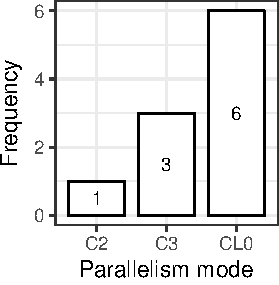
\includegraphics[width=0.32\textwidth]{plots/barplot-modes-static.pdf}
%% 	\caption{\label{fig:freqmodes-static}\Luis{This is wrong, it
%% 	should be \textbf{CF0} instead of \textbf{CL0}}Distribution of parallel modes
%%     identified statically in a subset of \numProjectsPar{} projects.
%%     A project may have support to more than one parallel mode.}
%% \end{figure}


\begin{itemize}
	\item \numRQAdoptionTwo{}. \textbf{\RQAdoptionTwo{}}
\end{itemize}

To answer this research question we surveyed developers involved in a
selection of projects from our benchmark with time-consuming test
suites.  The goal of the survey is to better comprehend developer's
attitude towards the use of parallelism as a mechanism to speedup
regression testing.  We surveyed developers from a total of
\emailsProjects{} projects.  From the initial list of \numMedLong{}
project, we discarded 11 projects that we knew a priori used
parallelization, and \discartedProjects{} projects that we could not find
developer's emails from commit logs.  From this list of projects, we
mined potential participants for our study.  More precisely, we
searched for developer's name and email from the last 20 commits to
the corresponding project repository.  Using this approach, we
identified a total of \emailsSent{} eligible participants.  Finally,
we sent plain-text e-mails, containing the survey, to those developers.  In
total, \emailsAnswered{} developers replied but we discarded
\emailsFalseAnswers{} replies with subjective answers.  Considering
projects covered by the answers, a total of \emailsProjectsAnswered{}
projects (\percEmailsProjectsAnswered{} of the total) were represented
in those replies.  Note that multiple developers on each project
received emails.  We sent the following set of questions to
developers:

\begin{enumerate}
\item How long does it take for tests to run in your environment? Can
  you briefly define your setup?
\item Do you confirm that your regression test suite does *not* run in parallel?
\item\label{questionThree} Select a reason for not using parallelization:
  \begin{enumerate}[label=\alph*)]
  \item I did not know it was possible
  \item I was concerned with concurrency issues
  \item I use a continuous integration server
  \item Some other reason. Please elaborate.
  \end{enumerate}
\end{enumerate}

%% \begin{enumerate}
%% 	\item How long does it take for test to run in your
%%		environment?
%%	\item Can you briefly define your setup?
%%	\item Do you confirm that your project does not run in
%%		parallel?
%%	\item Select a reason for not using paralellization:
%%		\begin{enumarate}
%%			\item I did not know it was possible;
%%			\item I was concerned with concurrency issues;
%%			\item I use a continuous integration server;
%%			\item Some other reason.
%%		\end{enumerate}
%% \end{enumerate}
%% One of the goals of the first questions is to identify potential
%% discrepancies between our experimental environment and the environment
%% of developers.  Overall, we found that \Fix{...}

Considering question 1, we confirmed that execution time was
compatible with the results we reported in Section~\ref{sec:rqA}.
Furthermore, \emailsCI{} of the participants indicated the use of
Continuous Integration (CI) to run tests, with \emailsDistributed{} of
these participants reporting that test suites are modularized and
those modules are tested independetly in CI servers through different
parameters.  Those participants argumented that such practice helps to
reduce time to observe test failures, which is the goal of speeding up
regression testing.  A total of \emailsLocal{} participants answered
that they do run tests in their local machines.  Note, however, that
CI does not preclude low-level parallelization.  For example,
installations of open-source CI tools (\eg{}, Jenkins~\cite{jenkins})
in dedicated servers would benefit from running tests faster through
low-level test suite parallelization.

% \emailsNotDescribed{} developers did not described their environment.

Considering question 2, the answers we collected indicated, to our
surprise, that six of the \emailsProjectsAnswered{} projects execute
tests in parallel.  This mismatch is justified by cases where neither
of our checks (static or dynamic) could detect presence of
parallelism.  A closer look at these projects revealed that one of
them contained a \emph{pom.xml} file encapsulated in a jar file
(similar case as reported in Section~\ref{sec:rqC-2}), in one of the
projects the particpant considered that distributed CI was a form of
parallelism, and in four projects the team preferred to implement
parallelization instead of using existing features from the testing
framework and the build system~---~in two projects the team
implemented concurrency control with custom JUnit test runners and in
two other projects the team implemented concurrency within test
methods.  Note that, considering these four extra cases (ignored two
distributed CI cases), the usage of parallelization increases from
\percentParallel{} to \percentParallelUpdated{}.  We do not consider
this change significant enough to modify our conclusion about
practical adoption of parallelization (\numRQAdoptionOne{}).

%% , one runs a manually created Thread to run some
%% tests, and the other runs in parallel by using Java 8 collection
%% streams, that allows the developers to iterate over a list in
%% parallel.

%% did not confirmed, however,
%% the developers confirmed the need of an extra parameter at the command
%% line to execute in parallel.

Considering question 3, the distribution of answers was as follows.  A
total of \emailsA{} of the \emailsProjectsAnswered{} developers who
answered the survey did not know that parallelism was available in
Maven (option ``a''), \emailsB{} of developers mentioned that they did
not use parallelism concerned with possible concurrency issues (option
``b''), \emailsD{} of developers mentioned that continuous integration
services sufficed to provide timely feedback while running only smoke
\begin{wrapfigure}{r}[0pt]{0pt}%0.525\linewidth
    \centering
    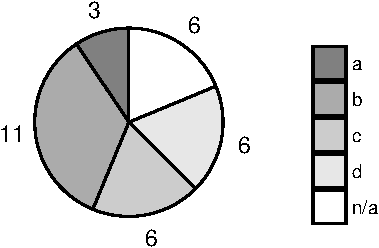
\includegraphics[width=.18\textwidth]{plots/survey.pdf}
    \caption{\label{fig:rq5-answers}Summary of developer's answers to
      survey question~\ref{questionThree}.}
\end{wrapfigure}
tests (\ie{}, short-running tests) locally (option ``c'')\Comment{here
  I want to say that they use it for something like "non-blocking
  testing" while developing in a local machine}, and \emailsD{} of
developers who provided an alternative answer (option ``d'') mentioned
that using parallelism was not worth the effort of preparing the test
suites to take advantage of available processing power.  A total of
\emailsNA{} of participants did not answer the last question of the
survey.  The pie chart in Figure~\ref{fig:rq5-answers} 
summarizes the distribution of answers.

\begin{center}
\fbox{
	\begin{minipage}{8cm}
	  \textit{Answering \numRQAdoptionTwo{}:}~\emph{Results suggest that dealing
       with concurrency issues (\ie{}, the extra work to organize test
       suite to safely explore concurrency) was the principal reason
       for developers not investing in parallelism.  Other reasons
       included availability of continuous integration services and
       unfamiliarity with the technology.}
	\end{minipage}
}
\end{center}

\subsection{Speedups}
\label{sec:rqD}

\begin{itemize}
    \item \numRQSpeedupOne{}. \textbf{\RQSpeedupOne}
\end{itemize}

To answer \numRQSpeedupOne{}, we considered the \numProjectsPar{}
subjects from our benchmark that use parallelization \emph{by default}
(see Figure~\ref{tab:freqmodes-dynamic}).  We compared running times
with parallelization~---~configured by project owners~---~and without
parallelization.

%% In those projects, parallelization is active without
%% passing any extra parameters.  Section~\ref{sec:rqC-1} describes in
%% detail the methodology we used to find these subjects.
%and
%Section~\ref{seq:rq6-tradeoffs}, we verified that both
%% executions produce the same outcome to eliminate noise from failing
%% tests.  To compute the speedup, we divide the time obtained in the
%% sequential execution by the time obtained from the default execution.
%% For instance, if a project runs the tests sequentially in $10m$ and
%% the same execution runs in $5m$ with parallelization enabled (default
%% execution), the speedup is two.

Figure~\ref{tab:speedup} summarizes results.  Lines are sorted by
project names.  Columns ``\emph{Group}'' and
``\emph{Name}'' indicate, respectively, the group and the name of the
subject.  Column ``$T_s$'' shows sequential execution time and column
``$T_p$'' shows parallel execution time. Column ``$T_s/T_p$'' shows
speedup or slowdown.  As usual, a ratio above 1x denotes speedup
and a ratio below 1x denotes slowdown.

\begin{figure}[h!]
\centering
\resizebox{.41\textwidth}{!}{%
  \scriptsize
\begin{tabular}{llrrr}
\toprule
\emph{Group} & \emph{Subject} & \multicolumn{1}{c}{$T_s$} & \multicolumn{1}{c}{$T_p$} & $T_s/T_p$ \\%
\midrule%
Medium & \Comment{BounceStorage }Chaos\Comment{ HTTP Proxy} & 1.51m & 1.47m & 
    \cellcolor{lightgray}1.01x\\%
Medium &\Comment{ Apache }Flink& 11.79m & 2.57m & 4.59x\\%
Long &\Comment{ Jenkins CI }Gerrit\Comment{ Plugin} & 51.19m & 40.31m &  1.26x\\%
Medium &\Comment{ Spotify }Helios& 4.46m & 1.63m & 2.73x\\%  
Medium &Javaslang& 2.18m & 1.82m & 1.19x\\%
Medium &Jcabi\Comment{ GitHub} & 2.76m & 0.30m &
    \cellcolor{lightgray}9.2x\\%
Medium &\Comment{ Hazelcast }Jet& 8.26m & 3.67m & 2.25x\\%
Long &\Comment{ Apache }Log4J2& 8.24m & 8.21m & \cellcolor{lightgray}1.00x\\%
Long &\Comment{ Jankotek }MapDB& 10.06m & 8.58m & 1.17x\\%
\midrule
\textbf{average} &  &  &  & \avgSpeedup{}x\\
\bottomrule%
\end{tabular}}
\caption{\label{tab:speedup}Speedup (or slowdown) of parallel
  execution ($T_p$) over sequential execution ($T_s$).  Default
  parallel configuration of Maven is used.  Highest slowdown/speedup
  appears in gray color.}
\end{figure}

Results indicate that, on average, parallel execution was
\avgSpeedup{} times faster compared to sequential execution.  Three
cases worth special attention: \CodeIn{Chaos}, \CodeIn{Jcabi} and
\CodeIn{Log4J2}.  No significant speedup was observed in
\CodeIn{Chaos}, a project with only three test classes, of which one
monopolizes the bulk of test execution time.  This project uses
configuration \ParClassSeqMeth{}, which runs test classes in parallel
and test methods, declared in each class, sequentially.  Consequently,
speedup cannot be obtained as the cost of the single expensive test
class cannot be broken down with the selected configuration.  Although
project \CodeIn{Jcabi} also uses configuration \ParClassSeqMeth{},
results obtained are very different compared to \CodeIn{Chaos}.  The
speedup observed in \CodeIn{Jcabi} was the highest amongst all
projects.  This project contains test classes with a small number of
test methods and several methods in those classes are time-consuming.
As result, the CPUs available for testing are kept occupied for the
most part during test execution.  Finally, we note that parallel
execution in \CodeIn{Log4J2} was innefective.  We found that Maven
invokes several test modules in this project but the test modules that
dominate execution time run sequentially by default.

%% The third, runs parallel configuration in
%% \Fix{80\%} of the project modules, however, the test time is dominated
%% by one of the sequentially running modules.  \Luis{$\leftarrow$ rework
%%   this} \Fix{falar sobre o resultado geral dos speedups - elaborar
%%   menor e maior speedup... acho que so vale a pena discutir quando
%%   tiver conviccao dos 2 casos}

\begin{center}
\fbox{
  \begin{minipage}{8cm}
    \textit{Answering \numRQSpeedupOne{}:}~\emph{Considering the
      machine setup we used, the average speedup observed with default
      configurations of parallelization was \avgSpeedup{}x.}
  \end{minipage}
}
\end{center}

\begin{itemize}
    \item \numRQSpeedupTwo{}. \textbf{\RQSpeedupTwo}
\end{itemize}

\newcommand{\subjectScalability}{MapDB}

This experiment evaluates the impact of making available to the build
system a growing number of CPUs for testing.  For that reason, we used
a machine with more cores compared to the one described in
Section~\ref{sec:setup}.  We used a Xeon E5-2660v2 (2.20GHz) Intel
processor machine with 80 virtual CPUs (40 cores with two native
threads each) and 256GB of memory, running Ubuntu 14.04 LTS Trusty
Tarr (64-bit version). This experiment uses configuration \ForkSeq{}
\begin{wrapfigure}{r}[0pt]{0pt}%0.525\linewidth
    \centering
    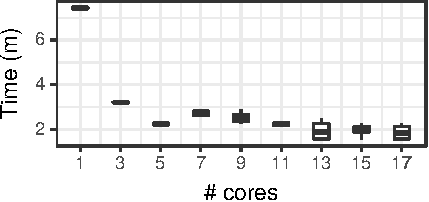
\includegraphics[width=.2\textwidth]{R/scalability/scalability.pdf}
    \caption{\label{fig:scalability}Scalability.}
\end{wrapfigure}
as the goal is to evaluate the impact on runtime of spawning a growing number of
JVMs in different CPUs.  Furthremore, we selected subject
\subjectScalability{} as it represents the case of a long-running test
suite (see Figure~\ref{tab:speedup}) with test cases distributed
across many test classes (194 test classes for \subjectScalability{}).
Note that a test class is the smallest unit that can be used to spawn
a test job on a JVM and that we have no control over which test
classes will be assigned to which JVM that the build system forks.

Figure~\ref{fig:scalability} shows the reduction of running times as
more CPUs contribute to the execution.  \Fix{elaborate...}

\begin{center}
\fbox{
  \begin{minipage}{8cm}
    \textit{Answering \numRQSpeedupTwo{}:}~\emph{...}
  \end{minipage}
}
\end{center}

\subsection{Issues}
\label{sec:rq6-tradeoffs}

This dimension assesses the impact of using distinct parallel
configurations on test flakiness (negative impact) and speedup
(positive impact).  Furthermore, note that Section~\ref{sec:rqD}
evaluated speedup in isolation, focused on projects configured to use
parallelism by default.

\begin{itemize}
    \item \numRQIssuesOne{}. \textbf{\RQIssuesOne{}}
\end{itemize}


%% The intuition is that efficiency and flakiness are inversely
%% proportional in some cases: if too many tests depends on the state of
%% a single external resource, several tests are likely to fail as the
%% degree of concurrency increases by exploiting maximum CPU usage.

%% Table header macros
% $\Uparrow_\text{speed}$
\newcommand{\subcolA}{$\text{speedup}$}
\newcommand{\subcolB}{$\%_\text{fail}$}
\newcommand{\colheader}[1]{\multicolumn{2}{c}{\emph{#1}}}
\newcommand{\blankentry}{\entry{-}{-}}
\newcommand{\subcol}{\subcolA{} & \subcolB{}}
\newcommand{\entry}[2]{#1 & #2}

\begin{figure*}[t]  
\centering
\small
\setlength{\tabcolsep}{3pt}
\begin{tabular}{l|rr|rr|rr|rr|rr|rr}
\toprule
\multirow{2}{*}{\emph{Subject (module)}} & \multicolumn{2}{c|}{\emph{\Seq}} &
    \colheader{\SeqClassParMeth} & \colheader{\ParClassSeqMeth} &
    \colheader{\ParClassParMeth} & \colheader{\ForkSeq} &
    \colheader{\ForkParMeth} \\ %\cline{2-12}
    & $T$ & $\mathit{N}$ & \subcol{} & \subcol{} & \subcol{} & \subcol{}
    & \subcol{}\\%
\midrule%
AWS SDK Java (\CodeIn{core})  & \entry{3.7m}{847}  & \entry{1.95x}{2.24\%} & \entry{2.47x}{2.77\%} & \entry{3.70x}{4.01\%} & \entry{}{} & \entry{}{}\\%

Facebook Linkbench    & \entry{4.3m}{98}  & \entry{1.00x}{0\%} & \entry{1.65x}{1.02\%} & \entry{1.59x}{1.02\%} & \entry{}{} & \entry{}{}\\%

GoogleCloud Dataflow Java (\CodeIn{sdk}) & \entry{1.6m}{3,345}  & \entry{1.23x}{1.67\%} & \entry{2.67x}{1.05\%} & \entry{0.80x}{5.35\%} & \entry{}{} & \entry{}{}\\%

Javaslang (\CodeIn{core})     & \entry{1.1m}{17,513}  & \entry{1.38x}{0\%} & \entry{1.83x}{0\%} & \entry{1.38x}{0\%} & \entry{}{} & \entry{}{}\\ 
JCabi Github                  & \entry{2.6m}{634} & \entry{2.10x}{0\%} & \entry{17.70x}{0\%} & \entry{28.80x}{0\%} & \entry{}{} & \entry{}{} \\
JCTools (\CodeIn{core})       & \entry{3.6m}{690}  & \entry{4.50x}{0\%} & \entry{3.60x}{0\%} & \entry{18.00x}{0\%} & \entry{}{} & \entry{}{}\\%
MapDB  & \entry{8.2m}{5,324}  & \entry{1.52x}{0\%} & \entry{2.73x}{0\%} & \entry{4.82x}{0.05\%}   & \entry{}{} & \entry{}{}\\%
Moquette                      & \entry{3.7m}{169} & \entry{4.62x}{65.64\%} & \entry{3.36x}{32.92\%} & \entry{12.33x}{77.78\%} & \entry{}{} & \entry{}{} \\
RipMe                         & \entry{1.1m}{54}  & \entry{0.94x}{0\%} & \entry{1.63x}{0\%} & \entry{1.63x}{0\%} & \entry{1.37x}{0\%} & \entry{1.42x}{0\%}\\
Stripe Java     & \entry{4.3m}{302}  & \entry{4.78x}{6.31\%} & \entry{3.31x}{7.31\%} & \entry{21.50x}{14.95\%} & \entry{}{} & \entry{}{}\\%





\midrule

\textbf{Average}   & \entry{-}{-} & \entry{-}{-} & \entry{-}{-} & \entry{-}{-}
& \entry{-}{-} & \entry{-}{-} \\%


%%  & \entry{x.xm}{0}  & \entry{}{\%} & \entry{}{\%} & \entry{}{\%} & \entry{}{} & \entry{}{}\\%
%%OpenMRS Core (\CodeIn{api})  & \entry{15.4m}{3436} & \blankentry{}        & \blankentry{}        & \blankentry{} & \entry{1.5x}{0\%} & \entry{1.7x}{0}\\%
%%Apache Flume (\CodeIn{core}) &  \entry{7.7m}{392}  & \blankentry{}        & \blankentry{}        & \blankentry{}       & \entry{0.9x}{0\%} & \blankentry{} \\%
%%Facebook Archive Linkbench   &  \entry{4.5m}{98}   & \entry{1.0x}{0.2\%}  & \entry{1.6x}{1.2\%}       & \entry{1.0x}{0\%}  & \entry{1.7x}{0.5\%}  & \entry{1.7x}{0.2\%}\\%
%%AWS SDK Java (\CodeIn{core}) &  \entry{3.8m}{847}  & \multicolumn{6}{c}{\Fix{requires investigation}} & \entry{2.2x}{0.1\%} & \entry{3.2x}{2.0\%}\\%

%% OpenMRS Core (\CodeIn{api})  & \entry{15.4m}{3436} & \blankentry{}        & \blankentry{}        & \blankentry{} & \entry{1.5x}{0\%} & \entry{1.7x}{0}\\%
%% Jankotek MapDB               &  \entry{9.9m}{5218} & \multicolumn{6}{c}{\cellcolor{lightgray}\emph{JVM Crash}} & \entry{1.5x}{0\%} & \entry{1.7x}{0\%}\\%
%% Apache Flume (\CodeIn{core}) &  \entry{7.7m}{392}  & \blankentry{}        & \blankentry{}        & \blankentry{}       & \entry{0.9x}{0\%} & \blankentry{} \\%
%% Apache Giraph (\CodeIn{core})&  \entry{7.2m}{236}  & \entry{2.1x}{5.1\%}  & \colheader{\cellcolor{lightgray}timeout}   & \entry{1.0x}{0\%} & \entry{1.0x}{0}\% & \colheader{\cellcolor{lightgray}JVM Crash}\\%
%% Facebook Archive Linkbench   &  \entry{4.5m}{98}   & \entry{1.0x}{0.2\%}  & \entry{1.6x}{1.2\%}       & \entry{1.0x}{0\%}  & \entry{1.7x}{0.5\%}  & \entry{1.7x}{0.2\%}\\%
%% Stripe Java                  &  \entry{4.2m}{302}  & \entry{4.2x}{5.2\%}  & \entry{3.5x}{5.7\%}       & \entry{4.2x}{6.3\%} & \entry{1.0x}{0.3\%} & \entry{4.2x}{5.7\%}\\%
%% AWS SDK Java (\CodeIn{core}) &  \entry{3.8m}{847}  & \multicolumn{6}{c}{\Fix{requires investigation}} & \entry{2.2x}{0.1\%} & \entry{3.2x}{2.0\%}\\%

%% Jenkins CI Github            & \entry{Xm}{Z}       & \entry{x}{\%}          & \entry{x}{\%} & \entry{x}{\%} & \entry{x}{\%} & \entry{x}{\%}\\%
%% Jenkins CI Docker Workflow   & \entry{Xm}{Z}       & \entry{x}{\%}          & \entry{x}{\%} & \entry{x}{\%} & \entry{x}{\%} & \entry{x}{\%}\\%
%% Hazelcast                    & \entry{Xm}{Z}       & \entry{x}{\%}          & \entry{x}{\%} & \entry{x}{\%} & \entry{x}{\%} & \entry{x}{\%}\\%

\bottomrule%
\end{tabular}
\caption{Speedup versus Flakiness (\subcolB). Configuration
  \emph{\Seq{}} denotes the comparison baseline, which runs tests
  sequentially.  Columns $T$ and $N$ indicate time and number of
  tests, respectively.  Other columns show speedup and percentage of
  failing tests in different configurations, compared to
  \emph{\Seq{}}.\Mar{Can you please add name of module for all subjects?}}
\label{tab:rq6-table}
\end{figure*}

To answer this research question, we conducted an experiment involving
the six parallel configurations from Section~\ref{sec:modes}  and the
top 10 long-running test modules from our sample set. The rationale
for this selection criteria was to maximize the chances of observing
speedup and flakiness, assuming that long-running tests also have many
tests. Indeed, we confirmed that test suites in these projects contain
at least 236 tests ($1,662.7$ in average). Also, we preferred to compare the
effect of a configuration over a single test module for projects with
multiple test modules.  Recall that large projects may contain several
test modules, and these modules may contain distinct characteristics
that could favor one configuration and not others; therefore, it would
be necessary to check each module individually for a fair comparison.
We are interested in understanding how efficiency (\ie, testing cost)
and flakiness (\ie, failing tests) are affected when we run a test
suite with different parallel configurations.  Recall that increased
resource contention obtained with parallelism can lead to concurrency
issues such as data races.  Flakiness and speedup are contradictory
forces that drive configuration selection.  We used as a \emph{control
group} (\ie, baseline) the sequential execution of each subject's
tests. Notice that for measuring flakiness, we have to consider only
tests that failed due to the concurrency in the parallel execution.
For that reason, we re-executed the tests in sequence ten times and
carefully verified that there are only passing tests in our baseline.
We considered ten as the number of re-executions based on the approach
used by Google reported in a previous work on test
flakiness~\cite{luo-etal-fse2014}.  To obtain parallel configurations,
we implemented a script that takes a subject and a configuration (\eg,
\ForkSeq{}) as inputs, and the script outputs the modified version of
the subject with the desired configuration. The workflow consists in
copying the project directory to a new directory, finding all existing
build files (\ie, \pomf{} files), and modifying all existing Maven
Surefire configurations with new values for the parameters
\CodeIn{parallel}, \CodeIn{forkCount}, and \CodeIn{threadCount} using
an XPath~\cite{xpath} library to manipulate XML documents. For
configurations with forked JVMs enabled (\ie, \ForkSeq{} and
\ForkParMeth{}), we changed the \CodeIn{forkCount} with the value
\CodeIn{1C} (\ie, one JVM per core).  To adjust the pool of threads
for parallelism within a JVM, we changed the parameter
\CodeIn{threadCount} with \Jbc{should we consider 2 as it is the
number of native threads per core OR 6 as it represents 3 Cores * 2
native threads?}.  To run the subjects and their respective variations
(\ie, the modified versions according to the parallelism
configuration), we used a similar approach as described in


Figure~\ref{fig:mvn-execution} except that we added a timeout of one
hour to run the tests. We used the \CodeIn{timeout}
command~\cite{timeout-cmd} to monitor the execution, and we configured
the command to dispatch a \emph{kill} signal if the test execution
exceeds the time limit. We imposed this time constraint to avoid
hanging indefinitely the experiment execution due to some thread
contention that may occur (\eg, deadlock). Finally, we saved each
execution log and XML test reports generated by Maven to collect the
execution time, the number of failing tests, and for reference to
analyze and diagnose outliers in our results. For efficiency, we
reported the speedup (\ie, $\Uparrow_\text{speed} = T_{\text{s}} /
T_{\text{p}}$) in average, and for flakiness, we reported the rate of
failing tests (\ie, $\mathit{\%_\text{fail} = failures / tests}$) in
average.  Figure~\ref{tab:rq6-table} summarizes the obtained results
ordered by the time cost (\ie, $T_\text{cost}$). \Fix{Remember to
explain efficiency cutoff, JVM crashes and timeout}

\Jbc{Lembrar que investigar o slowdown de Dataflow... os logs indicam que varios
dos testes que quebraram tentavam fazer uma autenticacao em algum servico.
Possivelmente o slowdown se deve ao tempo de resposta do servico quando
a autentiticao falha}

%% \begin{figure}[h!]
%% \centering
%% \resizebox{.48\textwidth}{!}{%
%% \begin{tabular}{lcrrrrr}
%% \toprule
%% \emph{Subject} & \emph{\# of tests} & \emph{\SeqClassParMeth{}} & \emph{\ParClassSeqMeth{}} & \emph{\ParClassParMeth{}} & \emph{\ForkSeq{}} & \emph{\ForkParMeth{}}\\%
%% \midrule%
%% Linkedin Pinot & 356 & - & - & - & - & -\\%
%% %% Jenkins CI Github Plugin & - & - & - & - & 0\% & -\\%
%% %% Kite SDK & - & - & - & - & - & -\\%
%% %% \Fix{!?} Apache Giraph & 327 & - & - & - & - & -\\%
%% %% OpenMRS Core & - & - & - & - & - & -\\%
%% %% Jenkins CI Docker Workflow Plugin & - & - & - & - & 0\% & -\\%
%% %% \Fix{Flaky} Apache Eagle & - & - & - & - & - & -\\%
%% %%Geotools & 7701 & - & - & - & - & -\\%
%% %%Kuromoji & 672 & - & - & - & - & -\\%
%% %%Atomix & 99 & - & - & - & - & -\\%
%% %%\Fix{Snazy OHC} & - & - & - & - & - & -\\%
%% %%\Fix{RoaringBitmap} & - & - & - & - & - & -\\%
%% \bottomrule%
%% \end{tabular}}
%% \caption{\Fix{Tabela de flakiness}}
%% \label{tab:rq6-flaky}
%% \end{figure}

\Fix{Elaborate results from efficiency}

\Fix{Elaborate results from flakiness}

\Fix{highlight special cases}

\Fix{Draw conclusions}

\begin{center}
\fbox{
\begin{minipage}{8cm}
\textit{Answering \numRQIssuesOne{}:~\emph{\Jbc{summarize findings...}}}
\end{minipage}
}
\end{center}

%%  LocalWords:  RQ occurence parallelization Tradeoffs API readme th
%%  LocalWords:  mvn clearcut escapeinside xleftmargin untestable LTS
%%  LocalWords:  framexleftmargin CPUs Tahr sysstat gh Vagrantfile
%%  LocalWords:  javadoc isolcpus JUnit's JUnitCore Gligoric boxplots
%%  LocalWords:  outliers apache uber chaperone facebookarchive
%%  LocalWords:  linkbench priori

%\chapter{Discussion}

This paper reports our finding on a study to evaluate impact and usage
of test suite parallelization, enabled by modern build systems and
testing frameworks.  This study is important given the importance to
speedup testing.  Note that test suite parallelization is
complementary to alternative approach to speedup testing
(see~Section~\ref{sec:related}).  The observations we made in this
study trigger multiple actions:

\begin{itemize}
\item \emph{Incentivize forking.}~Forked JVMs manifest low rates of
  test flakiness.  For instance, in \emph{\ForkSeq{}}, only 4 of 10
  projects manifest flakiness and, excluding the extreme case of
  \CodeIn{Moquette}, projects manifest flaky tests in low rates 0.23\%
  to 1.70\%.  Developers of projects with long-running test suites
  should consider using that feature, which is available in modern
  build systems today (\eg{}, Maven).
\item \emph{Break test dependencies.}~Non-forked JVMs can achieve
  impressive speedups at the expense of sometimes impressive rates of
  flakiness.  Breaking test dependencies to avoid flakiness and take
  full advantage of those options is advised for developers with
  greater interest in efficiency.
\item \emph{Refactor tests for load balancing.}~Forked JVMs scales
  better with the number of cores when the test workload is balanced
  across testing classes.  To balance the workload, automated
  user-oblivious refactoring can help in scenarios where developers
  are not willing to change test code but have access to machines with
  a high number of cores.
\item \emph{Improve debugging for build systems.}~While preparing our
  experiments, we found scenarios\Comment{, related to test
    parallelization,} where Maven's executions did not reflect
  corresponding JUnit's executions. \Comment{(Docker reproduction scripts
  available.)} Those issues can hinder developers from using parallel
  testing. Better debugging infrastructure is important.
\end{itemize}

This study brings to light the benefits and burdens of test suite
parallelization to improve test efficiency. It provides
recommendations to practitioners and developers of new techniques and
tools aiming to speed up test execution with parallelization.


%%  LocalWords:  parallelization Incentivize JVMs Moquette Refactor
%%  LocalWords:  refactoring JUnit's

%\section{Related Work}
\label{sec:related}
We discuss most related work in the following.
%% Researchers and practitioners have been shedding light to the demand
%% of techniques for optimizing test execution.

%% For instance, a recent paper from the automotive industry reported
%% that test suites can take days to run~\cite{artl-etal-icst2015}.
%% There are different aspects to consider when dealing with the
%% challenge of reducing test cost.

%ekstazi-web,
Regression testing research has focused mostly on test suite
minimization, prioritization, reduction, and
selection~\cite{yoo-harman-stvr2012,soetens-etal-2016}.  Most of these
techniques are unsoud (\ie{}, they do not guarantee that
fault-revealing tests will be considered for testing).  The test
selection technique
Ekstazi~\cite{gligoric-etal-issta2015,celik-etal-fse2017} is an
example of a sound regression testing technique. It conservatively
computes which tests have been impacted by file changes.  A test is
discarded for execution if it does not depend on any changed file
dynamically reachable from execution.\Comment{ Curiously Ekstazi's
  evaluation discovered subjects with parallelism enabled by
  default.}\Comment{ \c{C}elik~\etal{}~\cite{} recently extended
  Ekstazi to track files accessed outside JVM boundaries.} Important
to note that regression testing techniques, including test selection,
is complementary to test suite parallelization.

%\Luis{maybe we should create another division for test acceleration}

ElectricTest~\cite{bell-etal-esecfse2015} is a tool for efficiently
detecting data dependencies across test cases.  Dependency tracking is
important as to avoid test flakiness when parallelizing test
suites. ElectricTest observes reads and writes on global resources
made by tests to identify these dependencies at low cost. We remain to
investigate the impact of ElectricTest to reduce flakiness in
unrestricted test suite parallelization.

%% \textit{Usage of massively parallel hardware:}
%\textit{Hardware level massive parallelization:}

The use of the Single Instruction Multiple Data (SIMD) design has been
previoulsy explored in research to accelerate test
execution~\cite{damorim-etal-issta2007,damorim-etal-tse2008,kim-etal-issre2012,nguyen-etal-icse2014,rajan-etal-ase2014,sen-etal-fse2015,yaneva-etal-issta2017}. The
SIMD architecture, as implemented in modern GPUs, for instance, allows
the execution of a given instruction simultaneously against multiple
data.  For that reason, in principle, one test could be ran
simulteneously against multiple inputs provided that multiple test
inputs exist associated to that one test.  Recent
work~\cite{rajan-etal-ase2014,yaneva-etal-issta2017} explored that
idea to speedup test execution of embedded software using graphic
cards. Although benchmarks indicate superior performance compared to
traditional multicore CPUs, the use of the technology in broader
settings is limited. For example, execution of more general programs
can violate the SIMD's lock-step assumption on the control-flow of
threads.  This violation would affect negatively performance.
Furthermore, handling complex data is challenging in
SIMD~\cite{damorim-etal-issta2007,damorim-etal-tse2008}.  The approach
is promising when multiple input vectors exist for each test and the
testing code heavily manipulates scalar data types.  The datasets used
in those papers satisfied those constraints.


%% existing GPU programming-models (\eg{}, CUDA~\cite{cuda}, and
%% OpenCL~\cite{opencl}) are compatible only with a subset of the C/C++
%% language.
%% Recent work proposed a compiler-assisted approach to make programs
%% compatible with the relying programming-model used by
%% GPUs to parallelize tests~\cite{}.
%% \Jbc{...Justify they are out of scope for our subjects...}.

\Mar{can you complete this AND add text on high-level paralellism?}

\textit{Continuous integration services:}
Recent work showed us that Continuous Integration Services are widely
used and improve the productivity~\Fix{ref ref ref}. 

%% \Jbc{Missing work about testing in the cloud and Jon Bell}

\Comment{
\Fix{Please:
  (i) consider categorizing related work in sections  
  (ii) list papers that need to be discussed
  (iii) discuss papers that use multi-execution (SIMD cpus like GPUs)
  to speedup testing
  }
}
\Comment{
Similar approach to regression test selection has been recently
applied in the context of the GCC~\cite{gcc} configurable
system~\cite{souto-damorim-jss}.
O Trabalho de Hilton et al~\cite{hilton-etal-ase2016}, embora tenha
como objetivo entender o uso de CI, mostra que existe uma demanda em
acelerar o build e execucao de testes em servidores de integracao
    continua
}

%\chapter{Conclusion}

\section{Introduction}

\lipsum[1-4]

\section{Section}

\lipsum[2-4]

\subsection{Subsection}

\lipsum[2-4]

% References

\begin{references}
\bibliography{tmp}
\end{references}

% Appendix

%%\theappendix
%%\chapter{Mapping Study's Instruments}
\label{ap:mapping-study}

\begin{table}[!htp]
	\centering
	\caption{List of conferences on which the searches were performed.}
	\label{tbl:conferences_list}
	\rowcolors{2}{lightgray!30}{white}
	\resizebox{\columnwidth}{!}{
	\begin{tabular}{ll}
	\toprule
	\textbf{Acronym} & \textbf{Conference} \\
	\toprule
	APSEC & Asia Pacific Software Engineering Conference \\
	ASE   & IEEE/ACM International Conference on Automated Software Engineering \\
	CSMR  & European Conference on Software Maintenance and Reengineering \\
	ESEC  & European Software Engineering Conference \\
	ESEM  & International Symposium on Empirical Software Management and Measurement \\
	ICSE  & International Conference on Software Engineering \\
	ICSM  & International Conference on Software Maintenance \\
	ICST & International Conference on Software Testing \\
	InfoVis & IEEE Information Visualization Conference \\
	KDD   & ACM SIGKDD International Conference on Knowledge Discovery and Data Mining \\
	MSR   & Working Conference on Mining Software Repositories \\
	OOPSLA & Object-Oriented Programming, Systems, Languages and Applications \\
	QSIC  & International Conference On Quality Software \\
	SAC & ACM Symposium on Applied Computing \\
	SEAA & EUROMICRO Conference on Software Engineering and Advanced Applications\\
	SEDE & 19th International Conference on Software Engineering and Data Engineering \\
	SEKE  & International Conference on Software Engineering and Knowledge Engineering \\
	\bottomrule
	\end{tabular}
	}
\end{table}

\begin{table}[htp]
	\caption{List of journals in which the searches were performed.}
	\label{tbl:journals_list}
	\centering
	\rowcolors{2}{lightgray!30}{white}
	\begin{tabular}{l}
	\toprule
	\textbf{Journal title} \\
	\toprule
	ACM Transactions on Software Engineering and Methodology \\
	Automated Software Engineering \\
	Elsevier Information and Software Technology \\
	Elsevier Journal of Systems and Software \\
	Empirical Software Engineering \\
	IEEE Software \\
	IEEE Computer \\
	IEEE Transactions on Software Engineering \\
	International Journal of Software Engineering and Knowledge Engineering \\
	Journal of Software: Evolution and Process \\
	Software Quality Journal \\
	Journal of Software \\
	Software Practice and Experience Journal \\
	\bottomrule
	\end{tabular}
\end{table}

\begin{table}[h]
\centering
\footnotesize
 \rowcolors{2}{lightgray!30}{white}
\caption{Search string per Search Engine.}
\label{tbl:stringengine}
\begin{tabular}{p{.15\textwidth}p{.8\textwidth}}
\toprule
\textbf{Search Engine} & \textbf{Search String}\\
\toprule
   	 	Google Scholar &  bug report OR track OR triage ``change
   	 	request'' issue track OR request OR software OR ``modification request'' OR
   	 	``defect track'' OR ``software issue''  repositories maintenance evolution\\

   	 	ACM Portal & Abstract: "bug report" or Abstract:"change request"
   	 	or Abstract:"bug track" or Abstract:"issue track" or  Abstract:"defect
   	 	track" or Abstract:"bug triage" or Abstract: "software issue" or Abstract: "issue request"
   	 	or Abstract: "modification request") and  (Abstract:software or
   	 	Abstract:maintenance or Abstract:repositories or Abstract:repository \\

   	 	IEEExplorer (1) & (((((((((("Abstract": "bug report") OR
   	 	"Abstract":"change request") OR "Abstract":"bug track") OR "Abstract":"software issue") OR "Abstract":"issue request") OR
        "Abstract":"modification request") OR "Abstract":"issue track") OR
	    "Abstract":"defect track") OR "Abstract":"bug triage") AND
	    "Abstract":software)\\

         IEEExplorer (2) & (((((((((("Abstract": "bug report") OR
         "Abstract":"change request") OR "Abstract":"bug track") OR "Abstract":"software issue") OR
         "Abstract":"issue request") OR "Abstract":"modification request") OR
         "Abstract":"issue track") OR "Abstract":"defect track") OR
         "Abstract":"bug triage") AND "Abstract":maintenance)\\

         IEEExplorer (3) & (((((((((("Abstract": "bug report") OR
         "Abstract":"change request") OR "Abstract":"bug track") OR "Abstract":"software issue") OR
         "Abstract":"issue request") OR "Abstract":"modification request") OR
         "Abstract":"issue track") OR "Abstract":"defect track") OR
         "Abstract":"bug triage") AND "Abstract":repositories)\\

         IEEExplorer & (((((((((("Abstract": "bug report") OR
         "Abstract":"change request") OR "Abstract":"bug track") OR "Abstract":"software issue") OR
         "Abstract":"issue request") OR "Abstract":"modification request") OR
         "Abstract":"issue track") OR "Abstract":"defect track") OR
         "Abstract":"bug triage") AND "Abstract": repository)\\

         Citeseer Library & (abstract: "bug report" OR abstract:"change request" OR abstract:"bug track" OR abstract:"issue track" OR
	     abstract:"defect track" OR abstract:"bug triage" OR abstract: "software
	     issue" OR abstract: "issue request" OR abstract: "modification request")
	     AND (abstract:software OR abstract:maintenance OR abstract:repositories OR
	     abstract:repository)\\

	     Elsevier & ("bug report" OR "change
	     request" OR "bug track" OR "issue track" OR "defect track" OR "bug triage" OR "software issue" OR  "issue request" OR
	    "modification request") AND (software OR maintenance OR repositories OR
	    repository)\\

	    Scirus & ("bug report" OR "change request" OR "bug track" OR "issue track" OR  "defect track" OR "bug triage" OR
        "software issue" OR  "issue request" OR "modification request") AND
	    (software maintenance OR repositories OR repository) ANDNOT (medical OR
	    aerospace)\\

	    ScienceDirect & ("bug report" OR "change request" OR "bug track"
	     OR "issue track" OR "defect track" OR "bug triage" OR "issue request" OR
	     "modification request") AND LIMIT-TO(topics, "soft ware")\\

	     Scopus & ("bug report" OR "change request" OR "bug track" OR
	     "issue track" OR  "defect track" OR "bug triage" OR "software issue" OR
	     "issue request" OR "modification request") AND (software maintenance OR
	     repositories OR repository)\\

	     Wiley & ("bug report" OR "change request"
	     OR "bug track" OR "issue track" OR  "defect track" OR "bug triage" OR
         "software issue" OR  "issue request" OR "modification request") AND
	     (software maintenance OR repositories OR repository)\\

	     ISI Web\newline of Knowledge & ("bug report" OR "change request" OR "bug
	     track" OR "issue track" OR  "defect track" OR "bug triage" OR "software issue" OR  "issue request" OR "modification request") AND
	    (software maintenance OR repositories OR repository) ANDNOT (medical OR
	    aerospace)\\

	    SpringerLink & ("bug report" OR "change request" OR "bug track" OR "issue track" OR  "defect track" OR "bug triage" OR
        "software issue" OR  "issue request" OR "modification request") AND
	    (software maintenance OR repositories OR repository) ANDNOT (medical OR
	    aerospace)\\
	\bottomrule
\end{tabular}
\end{table}

\end{document}
